\chapter{Casos Analizados y Conjeturas}
\label{ch:caso_real}

En el capítulo \ref{ch:intro} se establecieron los cimientos teóricos que guiarán todo el trabajo: se revisaron las nociones básicas de polinomios ortogonales y sus matrices de momentos, se introdujo el operador de multiplicación \(\mathcal{D}\) y se formalizó la ortogonalidad de Sobolev junto con el problema central de la localización de ceros. Además, se contextualizó el estado del arte resaltando la utilidad de la aproximación matricial y de los estudios numéricos para desvelar la geometría de los ceros bajo diferentes productos internos.

El objetivo de este segundo capítulo es \emph{aplicar} aquel armazón teórico a los 4 casos concretos y, a partir de la evidencia obtenida, \emph{formular conjeturas} que orienten futuras demostraciones rigurosas. Con este fin, el capítulo se organiza en tres secciones principales:

\begin{itemize}
	\item \textbf{2.1 Caso real} - Se analizan productos de Sobolev definidos sobre soportes en la recta real. La simplicidad geométrica permite contrastar los resultados con referencias clásicas y calibrar las herramientas algebraicas presentadas anteriormente.
	\item \textbf{2.2 Caso circunferencia} - El estudio se traslada al plano complejo considerando medidas soportadas en circunferencias. Esta configuración pone de relieve la influencia de transformaciones de semejanza y la interacción entre la topología del soporte y la distribución de ceros.
	\item \textbf{2.3 Análisis y conjeturas} - Reúne las observaciones extraídas de ambos escenarios para proponer conjeturas sobre:
	      \begin{enumerate}
		      \item Cotas uniformes para los ceros en función del radio o de la posición relativa de los soportes.
		      \item El comportamiento asintótico de valores singulares sucesivos de las secciones \(\mathbf{D}_n\) y su relación con el radio espectral.
		      \item La influencia de la dominación secuencial o matricial en la acotación de \(\mathbf{D}\).
	      \end{enumerate}
\end{itemize}

A lo largo del capítulo se alternarán \emph{demostraciones analíticas} y \emph{experimentos numéricos}, reforzando la filosofía descrita en la introducción: combinar la teoría de matrices de Hessenberg con simulaciones para obtener una visión más completa de los ceros de los polinomios ortogonales de Sobolev.

\section{Caso Real}


\textbf{Ejemplo 1.}
$\langle p(t),q(t) \rangle_{\textbf{M}_S}=\int_{-1}^{1} p(t)q(t)t^2 \, dt + \int_{-1}^{1} p'(t)q'(t)t^{10} \, dt $

\begin{center}
	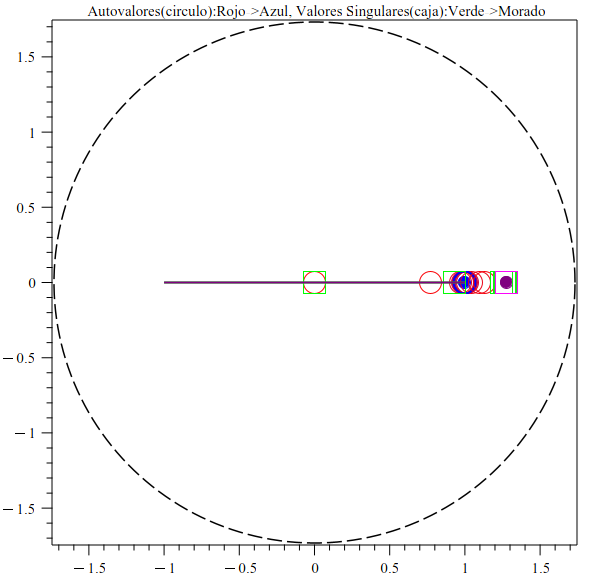
\includegraphics[width=0.9\textwidth]{include/a-1b1t2t10.png}

	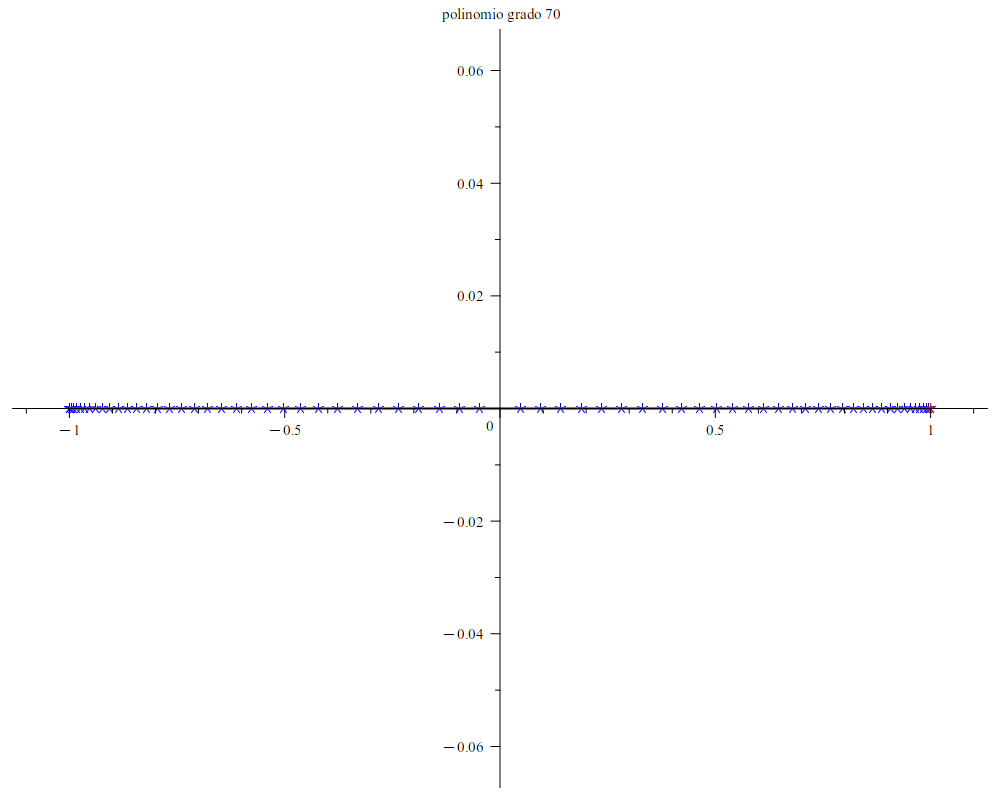
\includegraphics[width=0.9\textwidth]{include/a-1b1t2t10_zero.png}

	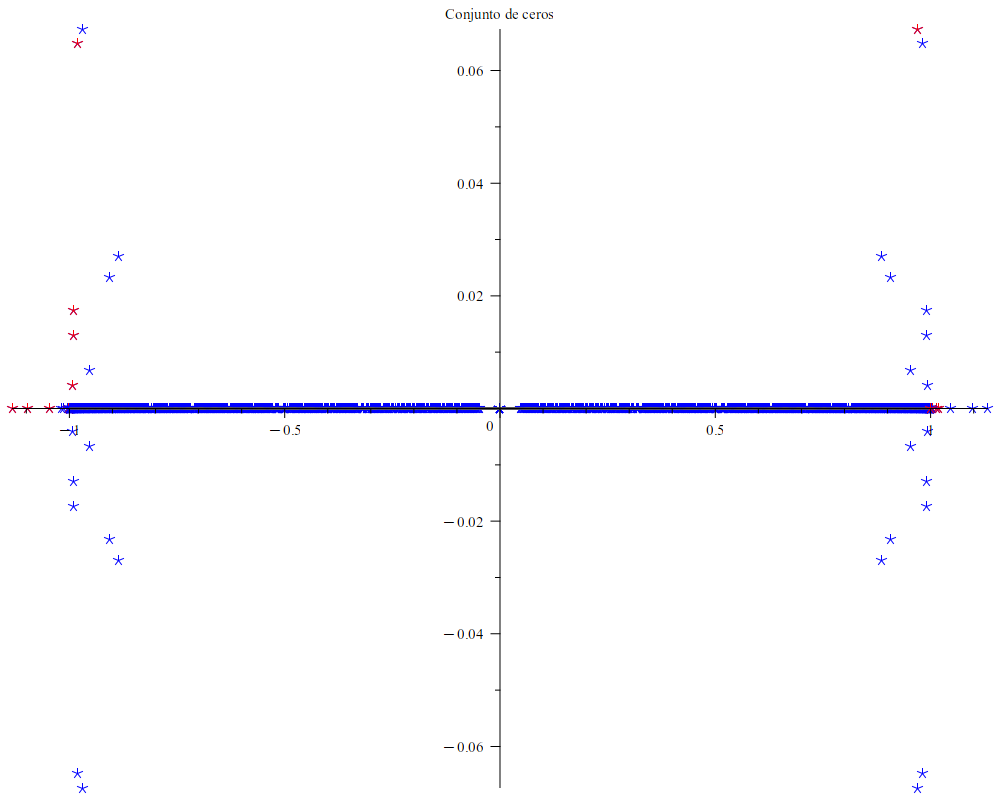
\includegraphics[width=0.9\textwidth]{include/a-1b1t2t10_zeros.png}
\end{center}

\begin{enumerate}
	\item $\lim_{n \to 50}\sigma_{1,n}=1.2760$
	\item $\lim_{n \to 50} \rho(\mathcal{D}_{n})=0.9999$
	\item $\max\{Z_{n}\}_{n=0}^{50}=1.1333$
	\item $\lim_{n \to 50}\sigma_{2,n}=1.2760$
\end{enumerate}

\textbf{Ejemplo 2.}
$\langle p(t),q(t) \rangle_{\textbf{M}_S}=\int_{-1}^{1} p(t)q(t)t^{10} \, dt + \int_{-1}^{1} p'(t)q'(t)t^{2} \, dt $

\begin{center}
	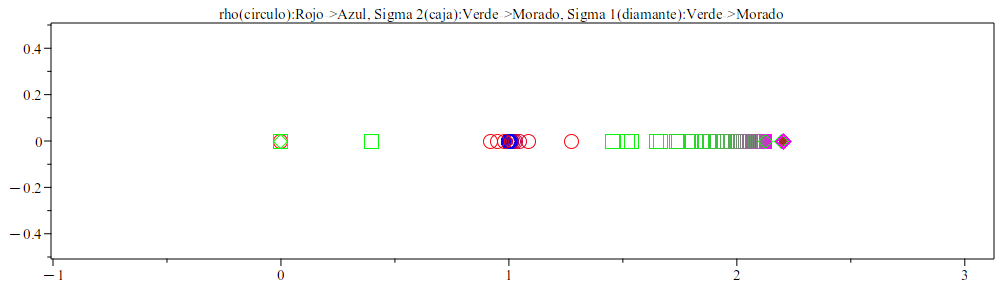
\includegraphics[width=0.9\textwidth]{include/a-1b1t10t2.png}

	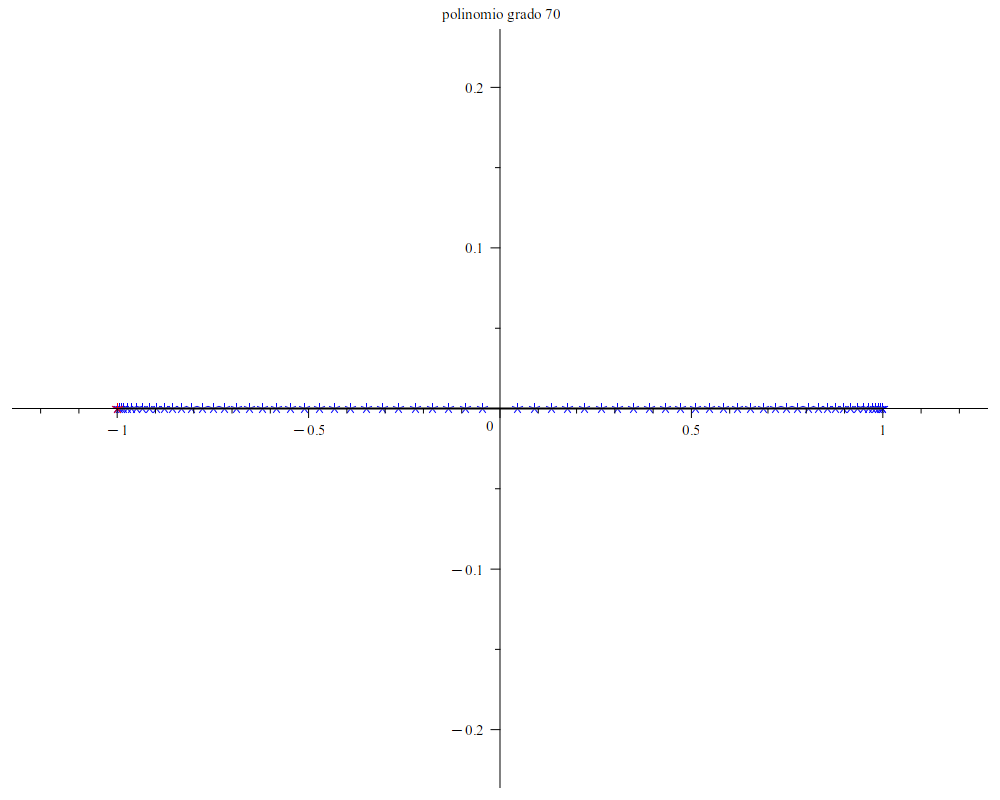
\includegraphics[width=0.9\textwidth]{include/a-1b1t10t2_zero.png}

	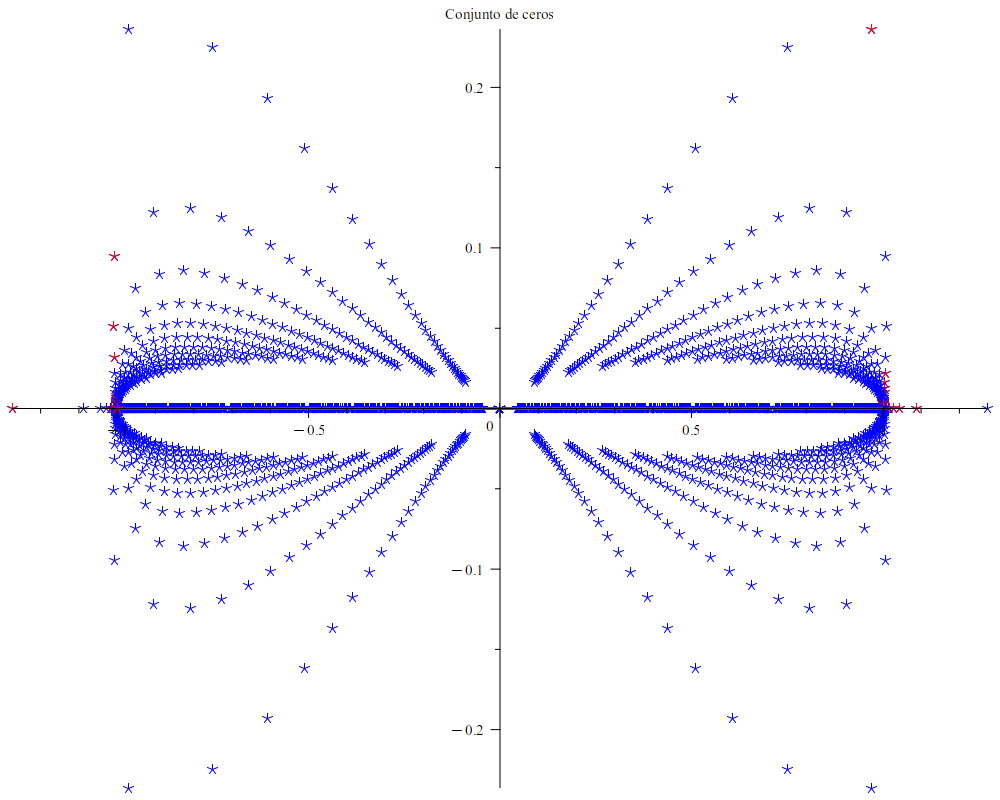
\includegraphics[width=0.9\textwidth]{include/a-1b1t10t2_zeros.png}
\end{center}

\begin{enumerate}
	\item $\lim_{n \to 50}\sigma_{1,n}=2.204$
	\item $\lim_{n \to 50} \rho(\mathcal{D}_{n})=1.000$
	\item $\max\{Z_{n}\}_{n=0}^{50}=1.275$
	\item $\lim_{n \to 50}\sigma_{2,n}=2.122$
\end{enumerate}


\textbf{Ejemplo 3.}
$\langle p(t),q(t) \rangle_{\textbf{M}_S}=\int_{0}^{10} p(t)q(t) \, dt + \int_{30}^{40} p'(t)q'(t) \, dt $

\begin{center}
	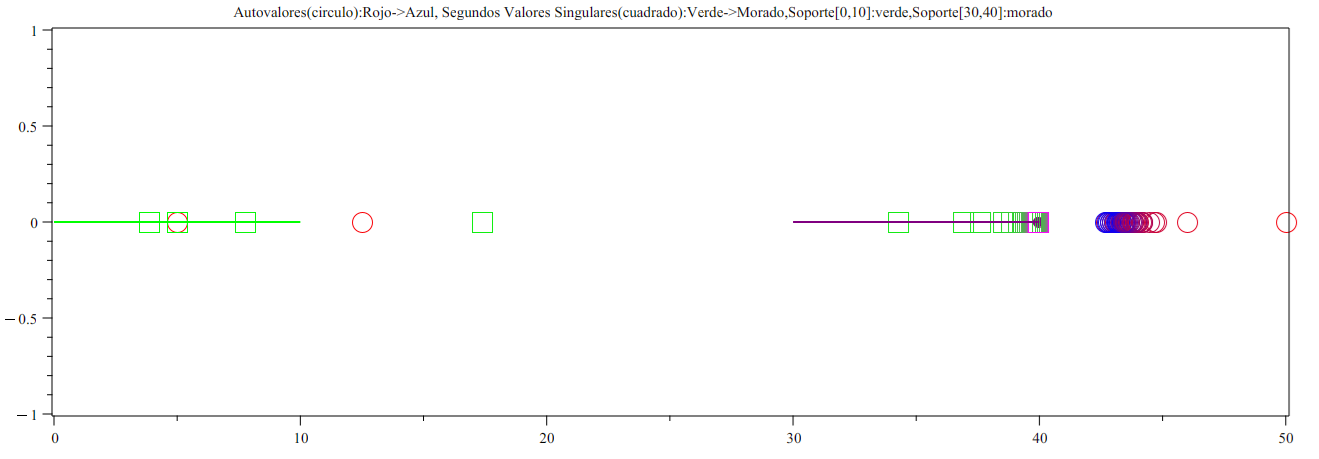
\includegraphics[width=0.9\textwidth]{include/a0b10c30d40.png}

	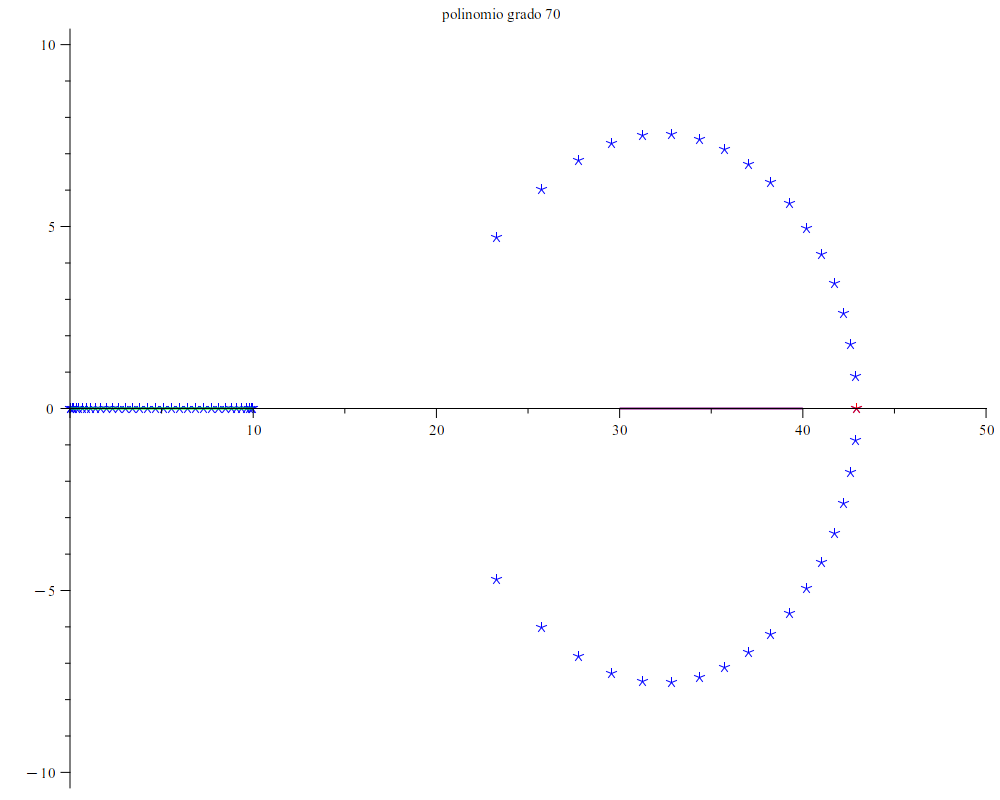
\includegraphics[width=0.9\textwidth]{include/a0b10c30d40_zero.png}

	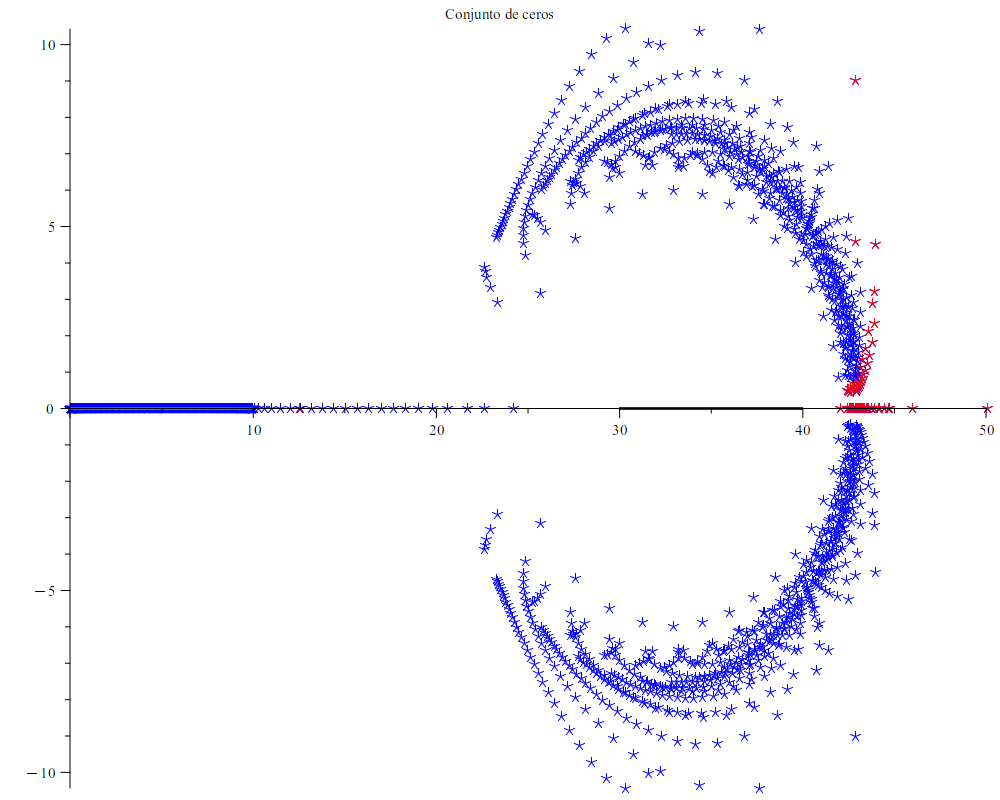
\includegraphics[width=0.9\textwidth]{include/a0b10c30d40_zeros.png}
\end{center}

\begin{enumerate}
	\item $\lim_{n \to 50}\sigma_{1,n}=9.272\times10^{16}$
	\item $\lim_{n \to 50} \rho(\mathcal{D}_{n})=42.930$
	\item $\max\{Z_{n}\}_{n=0}^{50}=50.052$
	\item $\lim_{n \to 50}\sigma_{2,n}=39.998$
\end{enumerate}

\textbf{Ejemplo 4.}
$\langle p(t),q(t) \rangle_{\textbf{M}_S}=\int_{30}^{40} p(t)q(t) \, dt + \int_{0}^{10} p'(t)q'(t) \, dt $

\begin{center}
	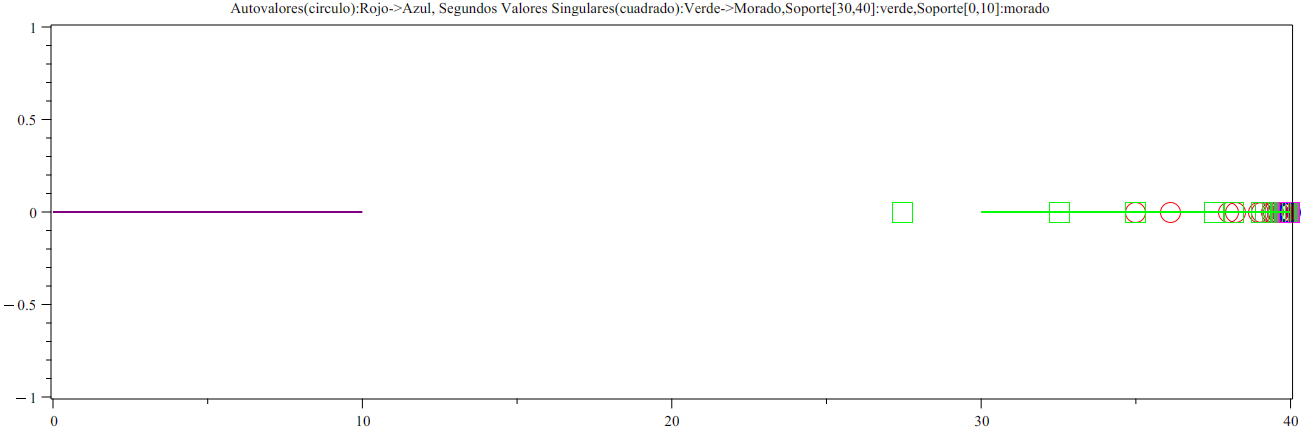
\includegraphics[width=0.9\textwidth]{include/a30b40c0d10.png}

	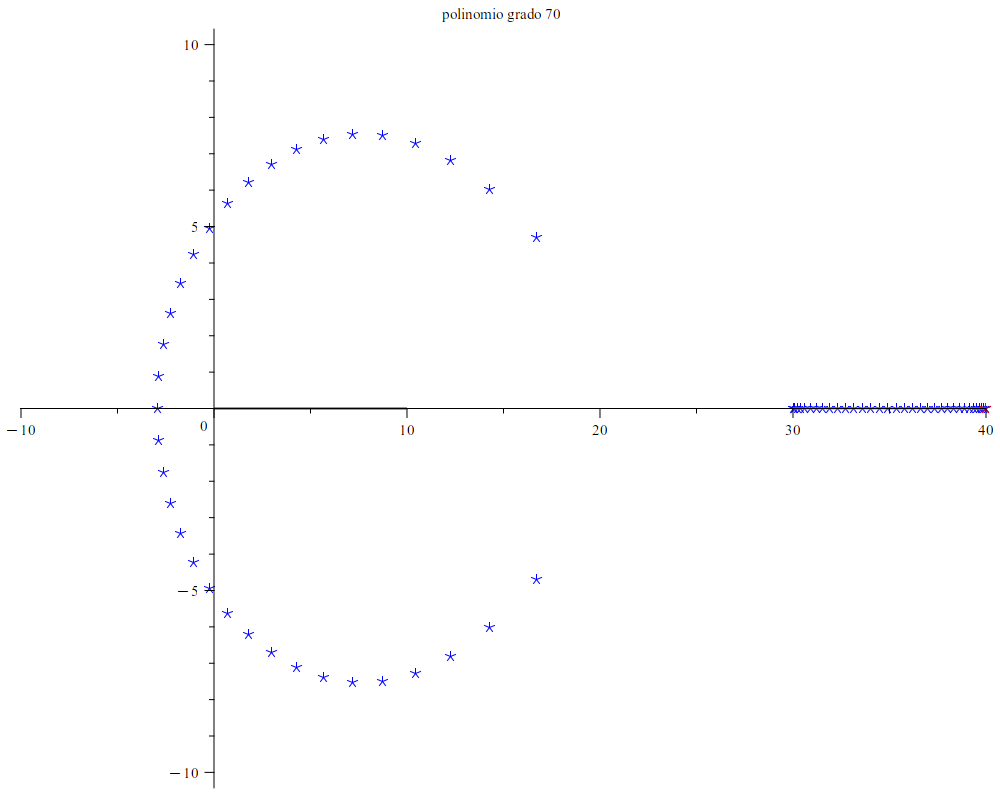
\includegraphics[width=0.9\textwidth]{include/a30b40c0d10_zero.png}

	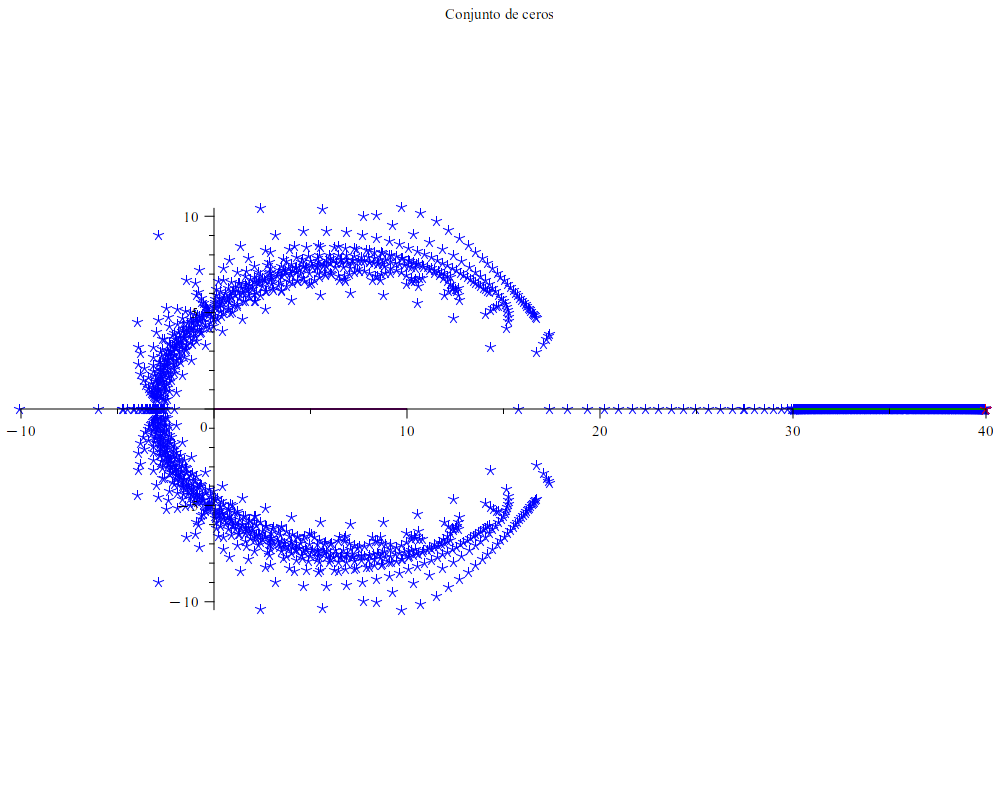
\includegraphics[width=0.9\textwidth]{include/a30b40c0d10_zeros.png}
\end{center}

\begin{enumerate}
	\item $\lim_{n \to 50}\sigma_{1,n}=9.272\times10^{16}$
	\item $\lim_{n \to 50} \rho(\mathcal{D}_{n})=39.991$
	\item $\max\{Z_{n}\}_{n=0}^{50}=39.991$
	\item $\lim_{n \to 50}\sigma_{2,n}=39.991$
\end{enumerate}

\textbf{Ejemplo 5.}
$\langle p(t),q(t) \rangle_{\textbf{M}_S}=\int_{0}^{10} p(t)q(t) \, dt + \int_{30}^{50} p'(t)q'(t) \, dt $

\begin{center}
	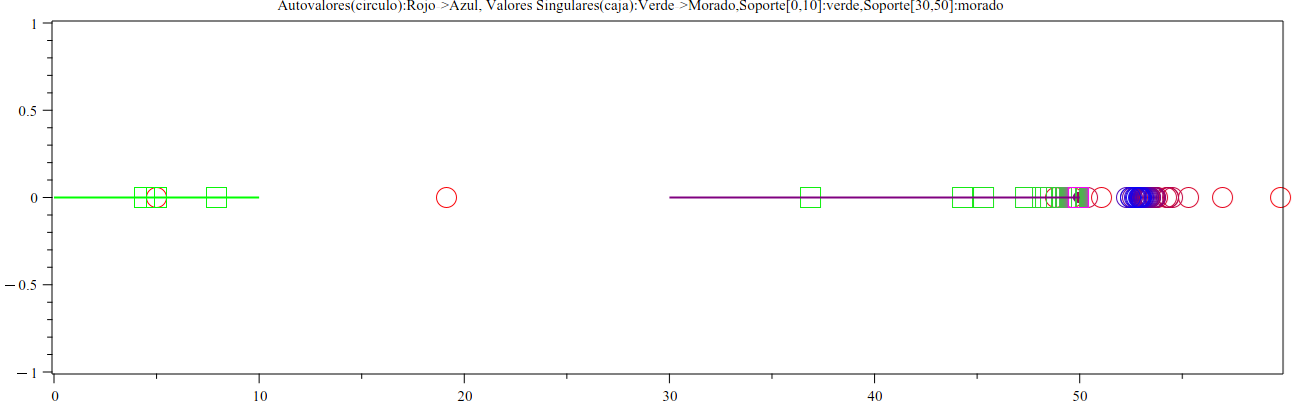
\includegraphics[width=0.9\textwidth]{include/a0b10c30d50.png}

	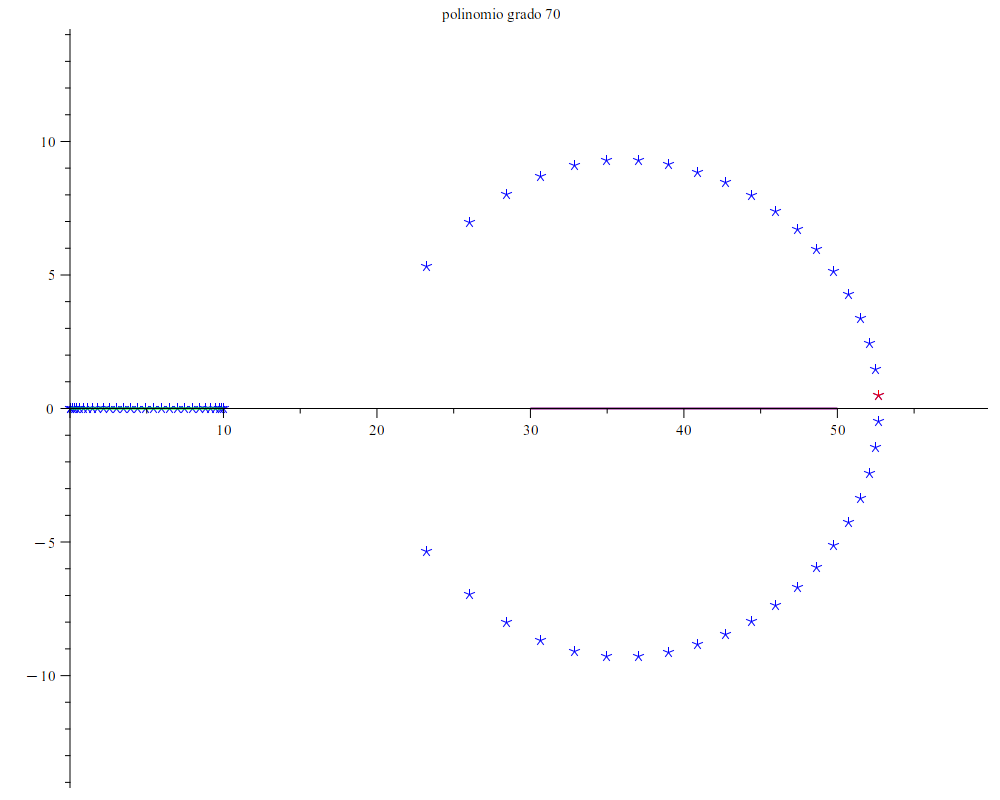
\includegraphics[width=0.9\textwidth]{include/a0b10c30d50_zero.png}

	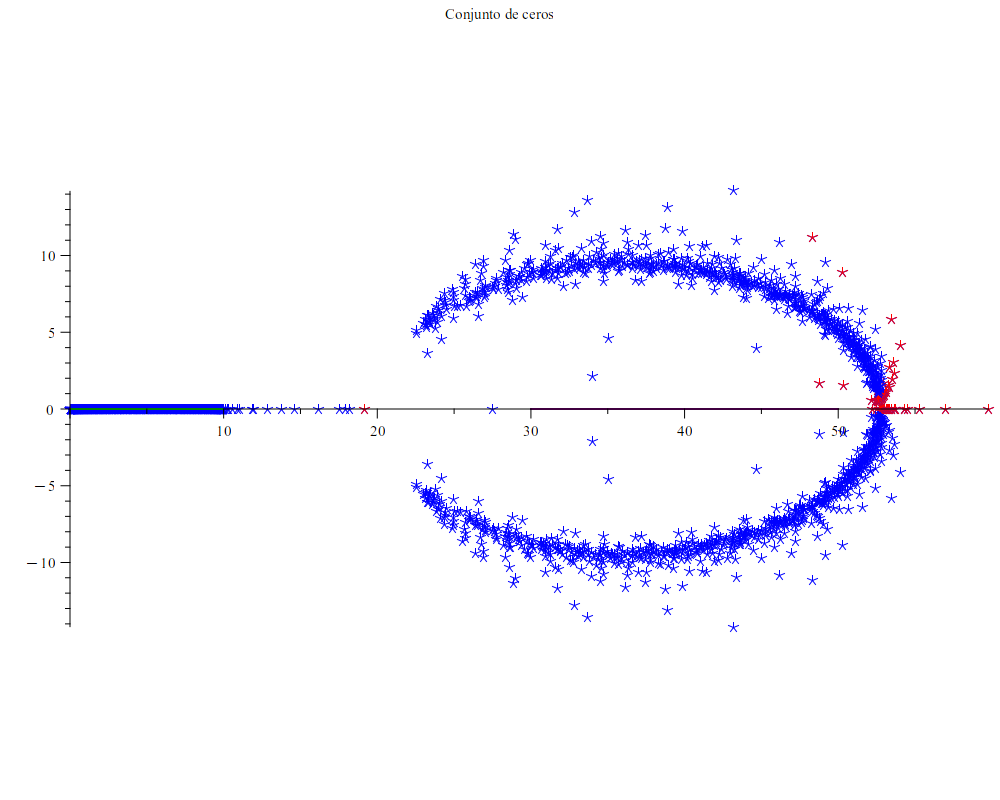
\includegraphics[width=0.9\textwidth]{include/a0b10c30d50_zeros.png}
\end{center}

\begin{enumerate}
	\item $\lim_{n \to 50}\sigma_{1,n}=5.990\times10^{13}$
	\item $\lim_{n \to 50} \rho(\mathcal{D}_{n})=52.656$
	\item $\max\{Z_{n}\}_{n=0}^{50}=59.814$
	\item $\lim_{n \to 50}\sigma_{2,n}=49.983$
\end{enumerate}

\textbf{Ejemplo 6.}
$\langle p(t),q(t) \rangle_{\textbf{M}_S}=\int_{30}^{50} p(t)q(t) \, dt + \int_{0}^{10} p'(t)q'(t) \, dt $

\begin{center}
	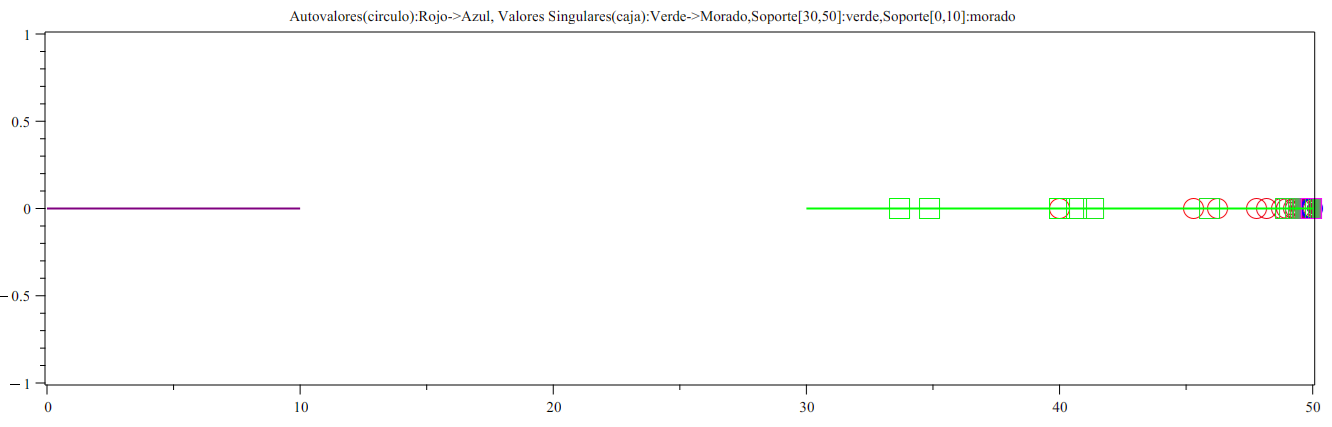
\includegraphics[width=0.9\textwidth]{include/a30b50c0d10.png}

	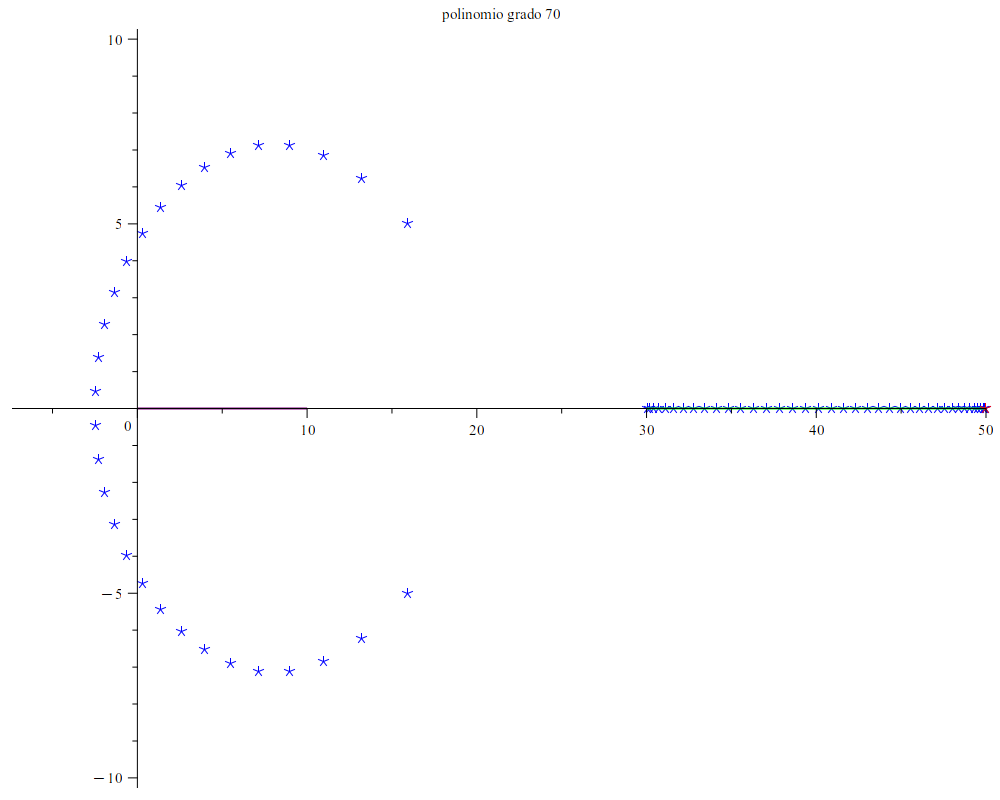
\includegraphics[width=0.9\textwidth]{include/a30b50c0d10_zero.png}

	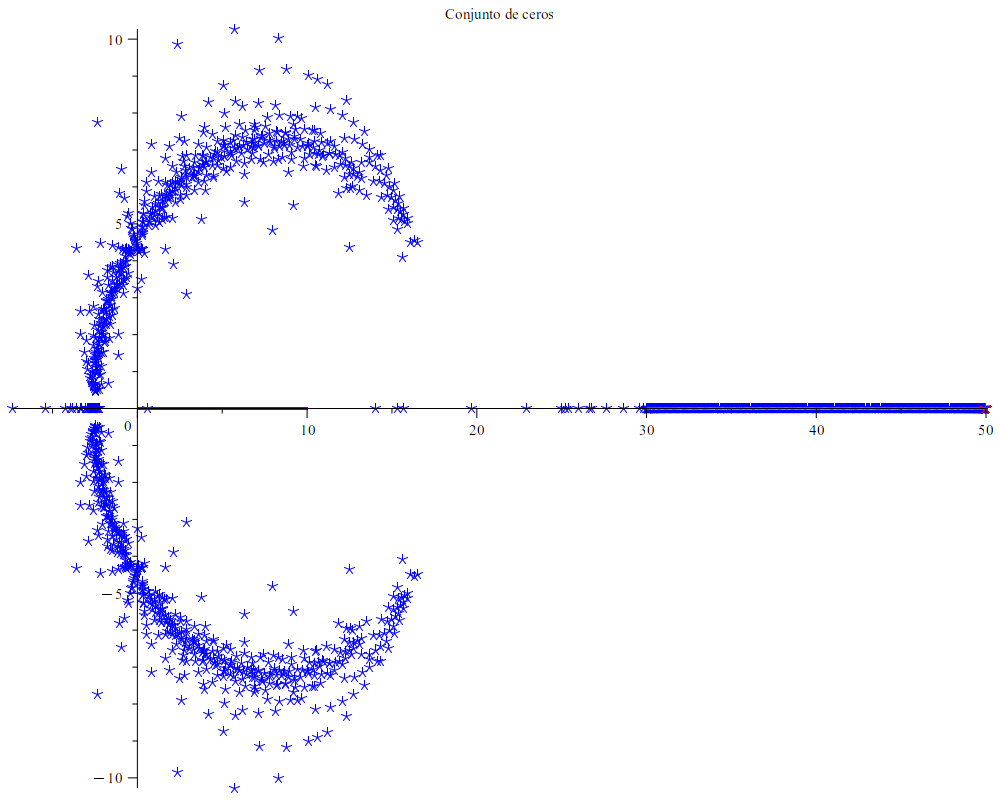
\includegraphics[width=0.9\textwidth]{include/a30b50c0d10_zeros.png}
\end{center}

\begin{enumerate}
	\item $\lim_{n \to 50}\sigma_{1,n}=3.752\times10^{13}$
	\item $\lim_{n \to 50} \rho(\mathcal{D}_{n})=49.987$
	\item $\max\{Z_{n}\}_{n=0}^{50}=49.987$
	\item $\lim_{n \to 50}\sigma_{2,n}=49.987$
\end{enumerate}

\textbf{Ejemplo 7.}
$\langle p(t),q(t) \rangle_{\textbf{M}_S}=\int_{0}^{20} p(t)q(t) \, dt + \int_{30}^{40} p'(t)q'(t) \, dt $

\begin{center}
	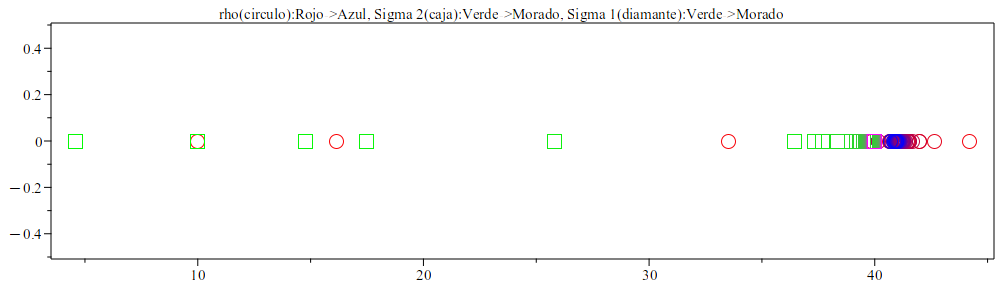
\includegraphics[width=0.9\textwidth]{include/a0b20c30d40.png}

	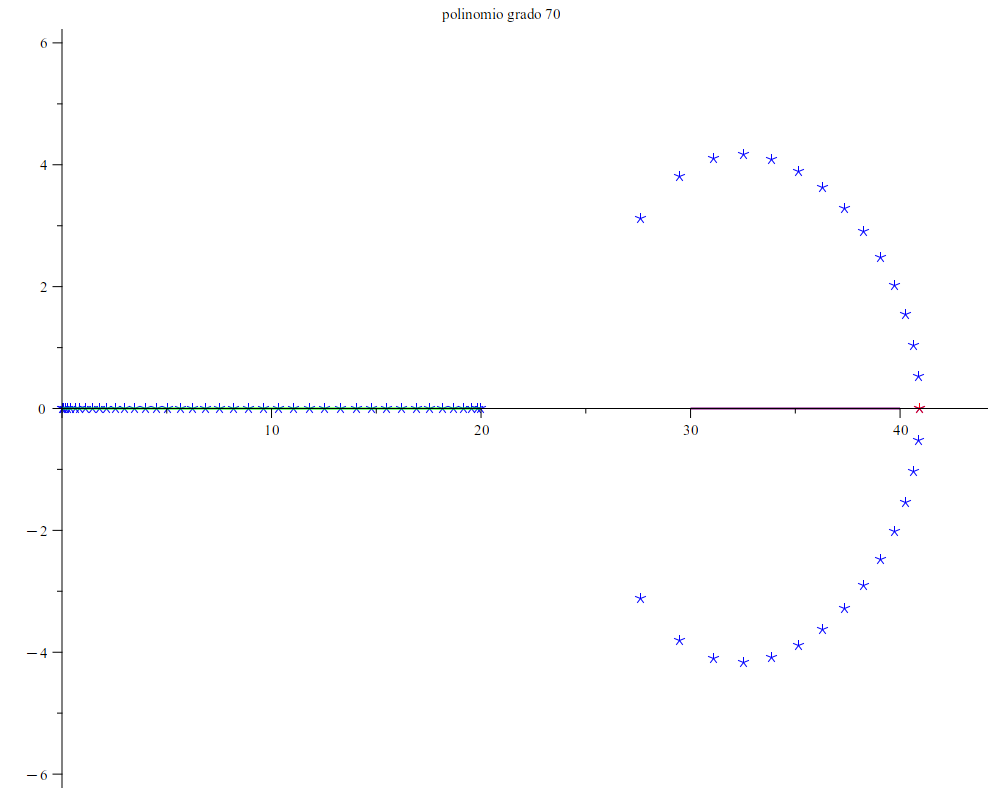
\includegraphics[width=0.9\textwidth]{include/a0b20c30d40_zero.png}

	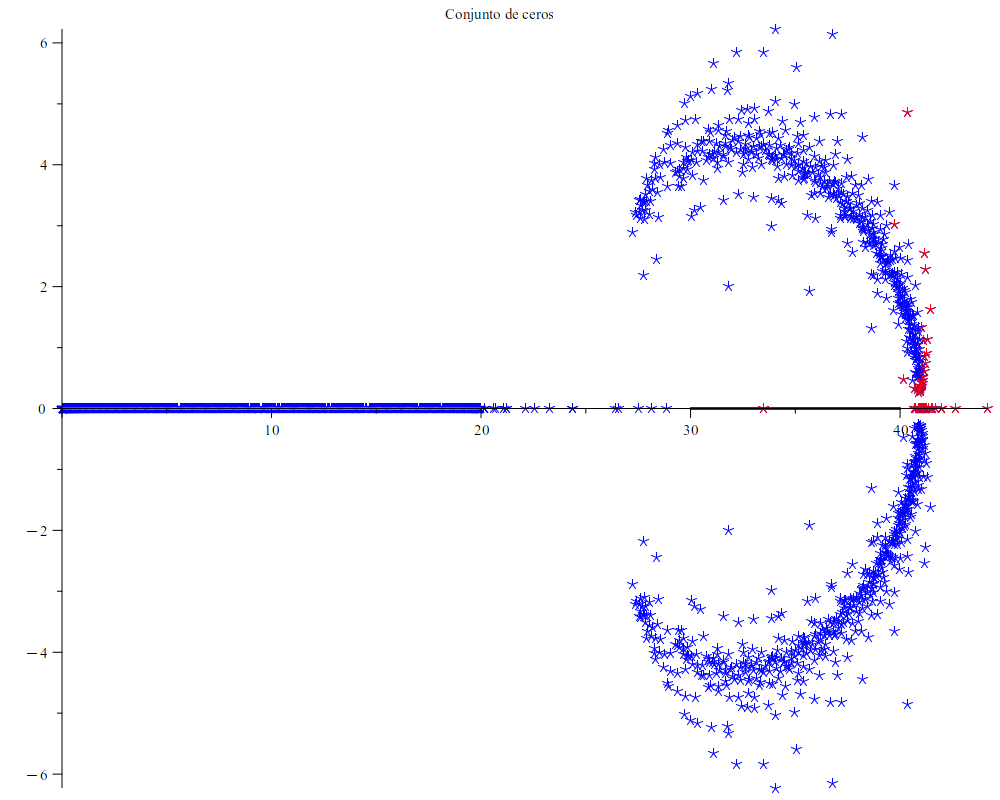
\includegraphics[width=0.9\textwidth]{include/a0b20c30d40_zeros.png}
\end{center}

\begin{enumerate}
	\item $\lim_{n \to 50}\sigma_{1,n}=2.944\times10^{9}$
	\item $\lim_{n \to 50} \rho(\mathcal{D}_{n})=40.951$
	\item $\max\{Z_{n}\}_{n=0}^{50}=44.196$
	\item $\lim_{n \to 50}\sigma_{2,n}=39.985$
\end{enumerate}

\textbf{Ejemplo 8.}
$\langle p(t),q(t) \rangle_{\textbf{M}_S}=\int_{30}^{40} p(t)q(t) \, dt + \int_{0}^{20} p'(t)q'(t) \, dt $

\begin{center}
	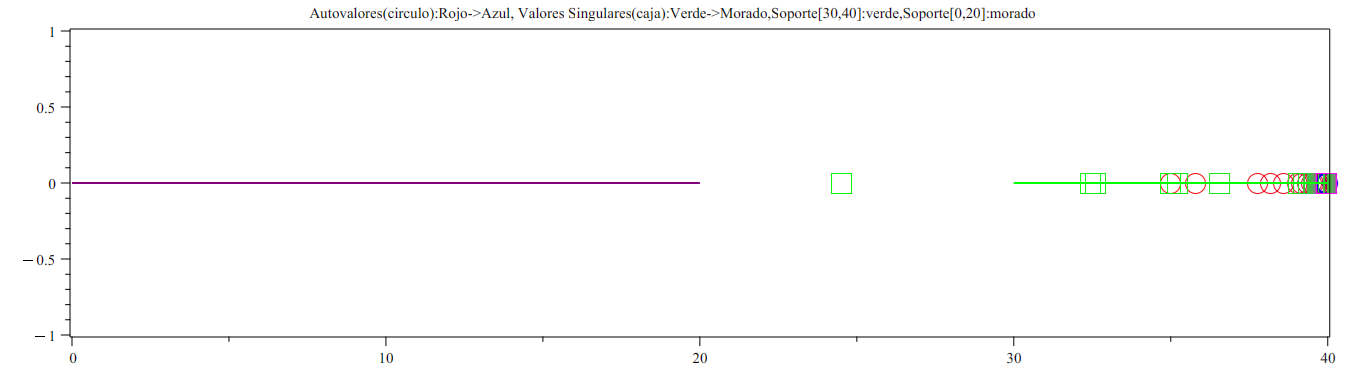
\includegraphics[width=0.9\textwidth]{include/a30b40c0d20.png}

	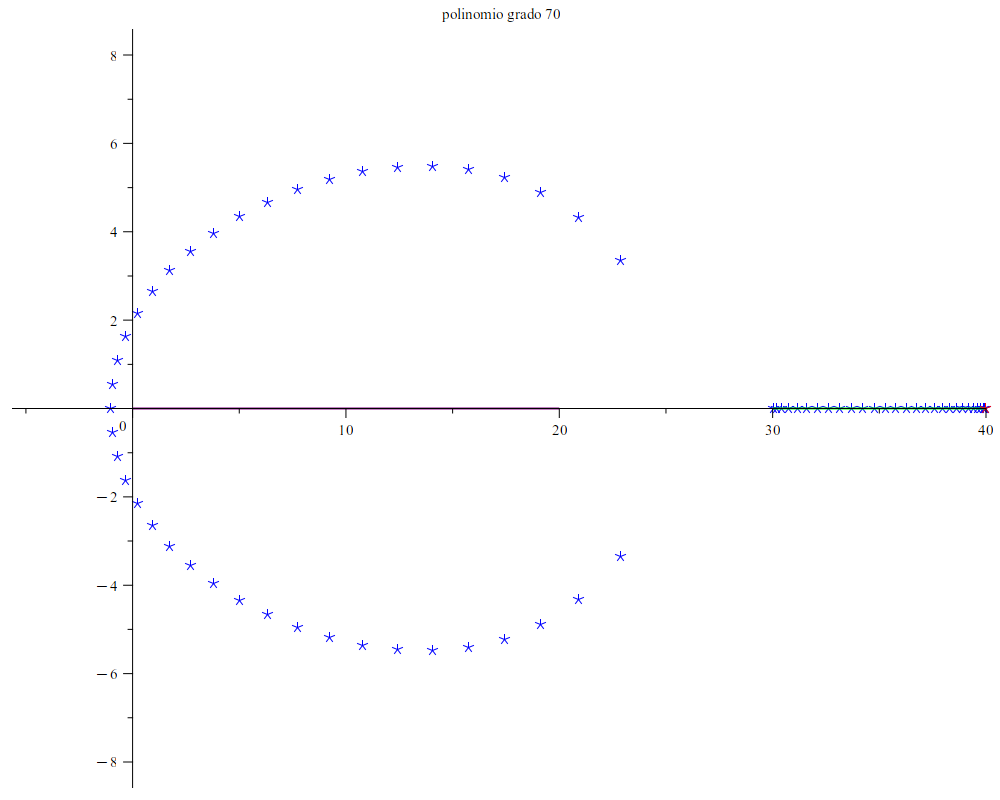
\includegraphics[width=0.9\textwidth]{include/a30b40c0d20_zero.png}

	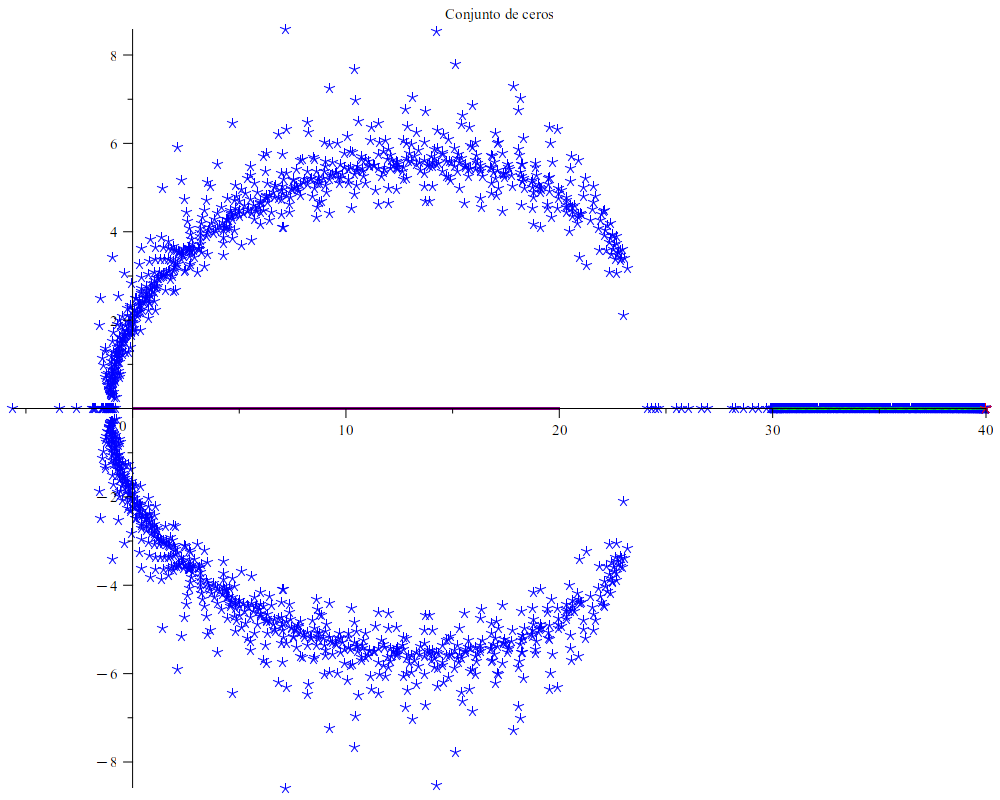
\includegraphics[width=0.9\textwidth]{include/a30b40c0d20_zeros.png}
\end{center}

\begin{enumerate}
	\item $\lim_{n \to 50}\sigma_{1,n}=4.136\times10^{8}$
	\item $\lim_{n \to 50} \rho(\mathcal{D}_{n})=39.989$
	\item $\max\{Z_{n}\}_{n=0}^{50}=39.989$
	\item $\lim_{n \to 50}\sigma_{2,n}=39.989$
\end{enumerate}

\textbf{Ejemplo 9.}
$\langle p(t),q(t) \rangle_{\textbf{M}_S}=\int_{-15}^{-5} p(t)q(t) \, dt + \int_{5}^{16} p'(t)q'(t) \, dt $

\begin{center}
	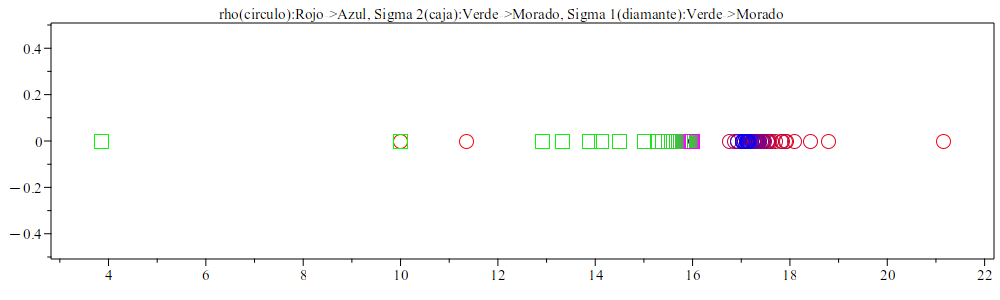
\includegraphics[width=0.9\textwidth]{include/a-15b-5c5d16.png}

	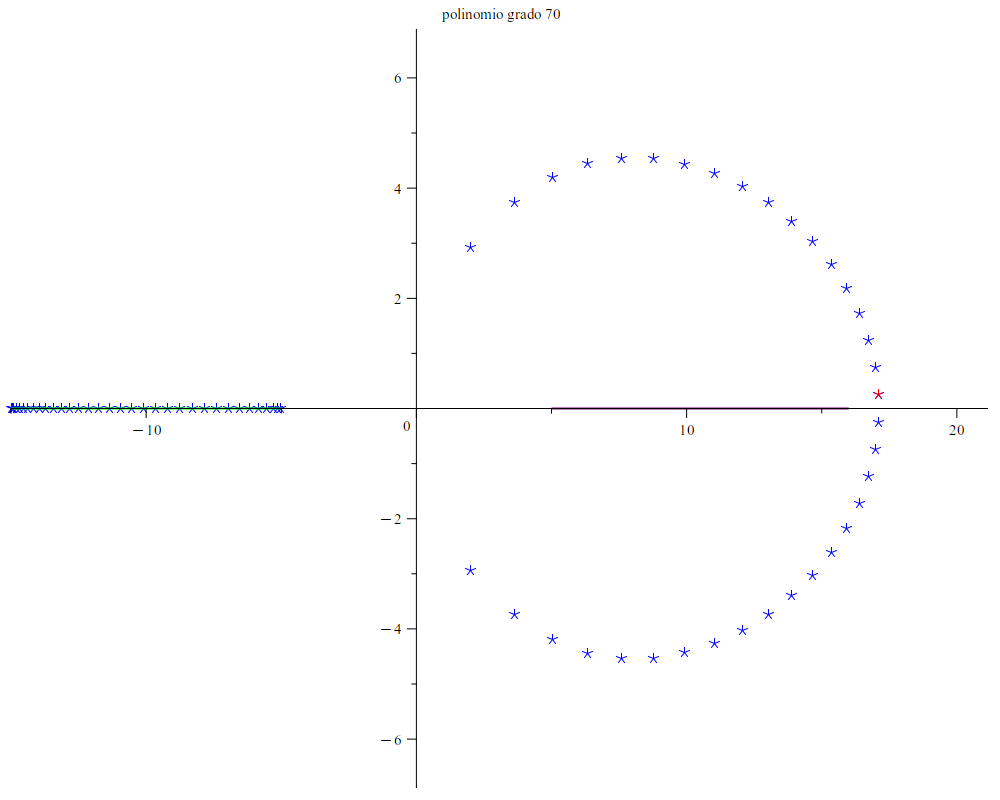
\includegraphics[width=0.9\textwidth]{include/a-15b-5c5d16_zero.png}

	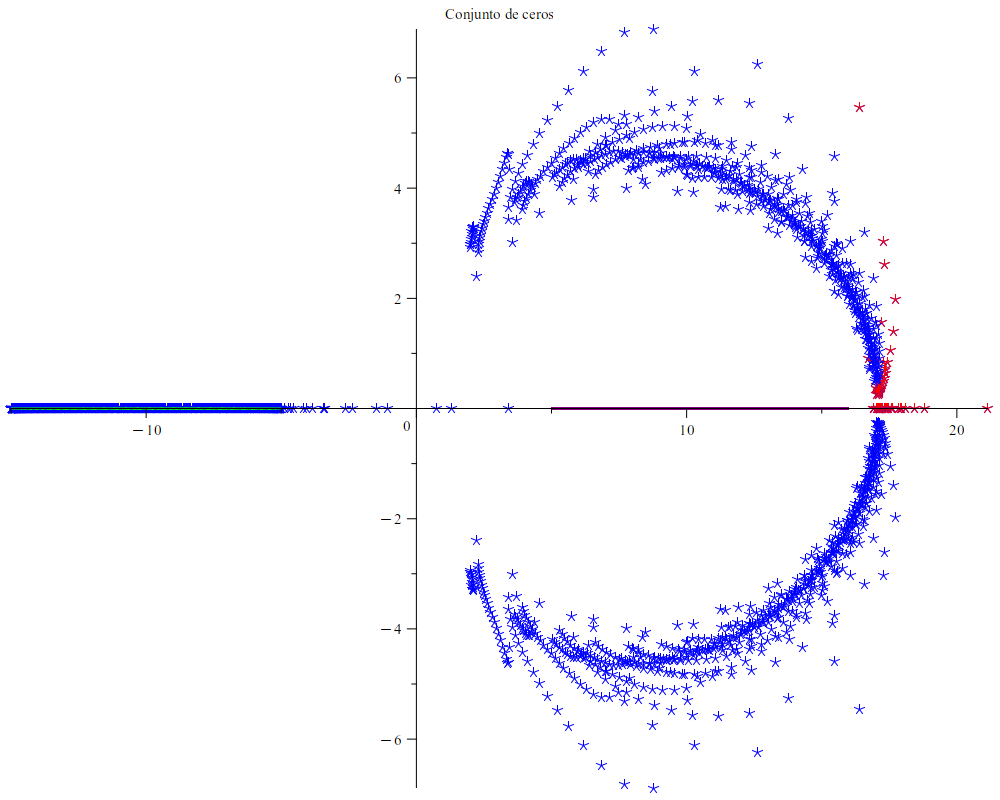
\includegraphics[width=0.9\textwidth]{include/a-15b-5c5d16_zeros.png}
\end{center}

\begin{enumerate}
	\item $\lim_{n \to 50}\sigma_{1,n}=3.711\times10^{10}$
	\item $\lim_{n \to 50} \rho(\mathcal{D}_{n})=17.107$
	\item $\max\{Z_{n}\}_{n=0}^{50}=21.152$
	\item $\lim_{n \to 50}\sigma_{2,n}=15.990$
\end{enumerate}

\textbf{Ejemplo 10.}
$\langle p(t),q(t) \rangle_{\textbf{M}_S}=\int_{-15}^{-5} p(t)q(t) \, dt + \int_{5}^{14} p'(t)q'(t) \, dt $

\begin{center}
	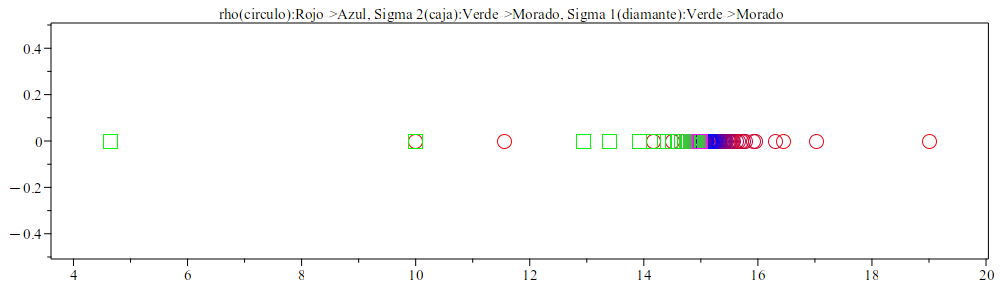
\includegraphics[width=0.9\textwidth]{include/a-15b-5c5d14.png}

	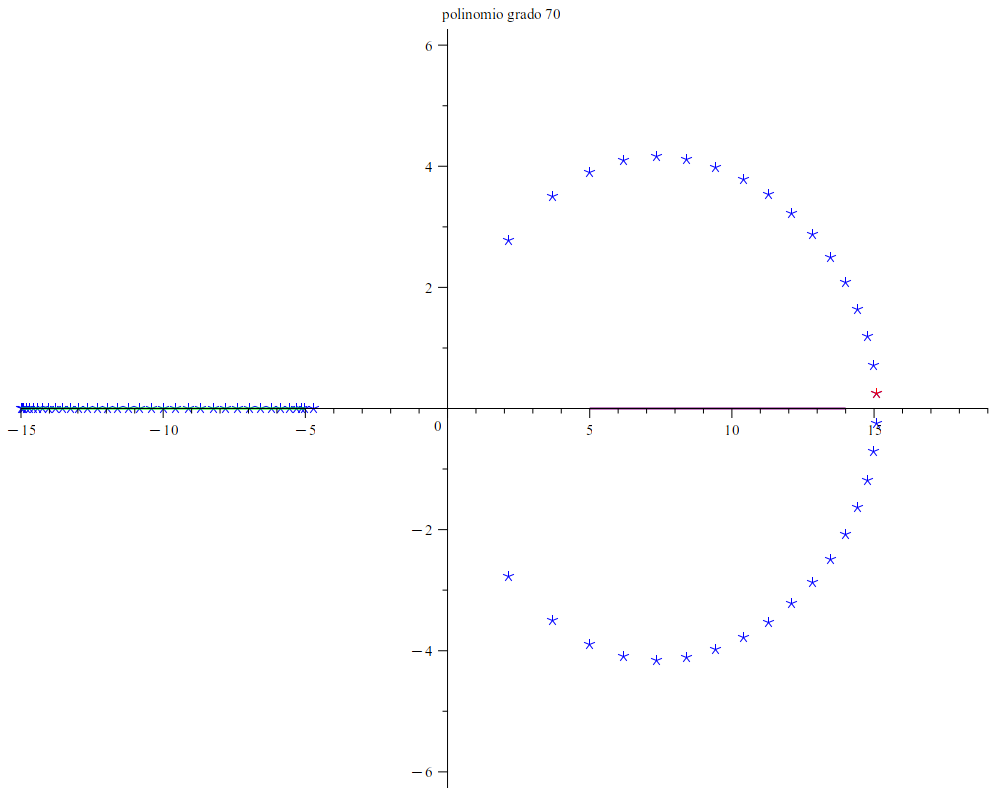
\includegraphics[width=0.9\textwidth]{include/a-15b-5c5d14_zero.png}

	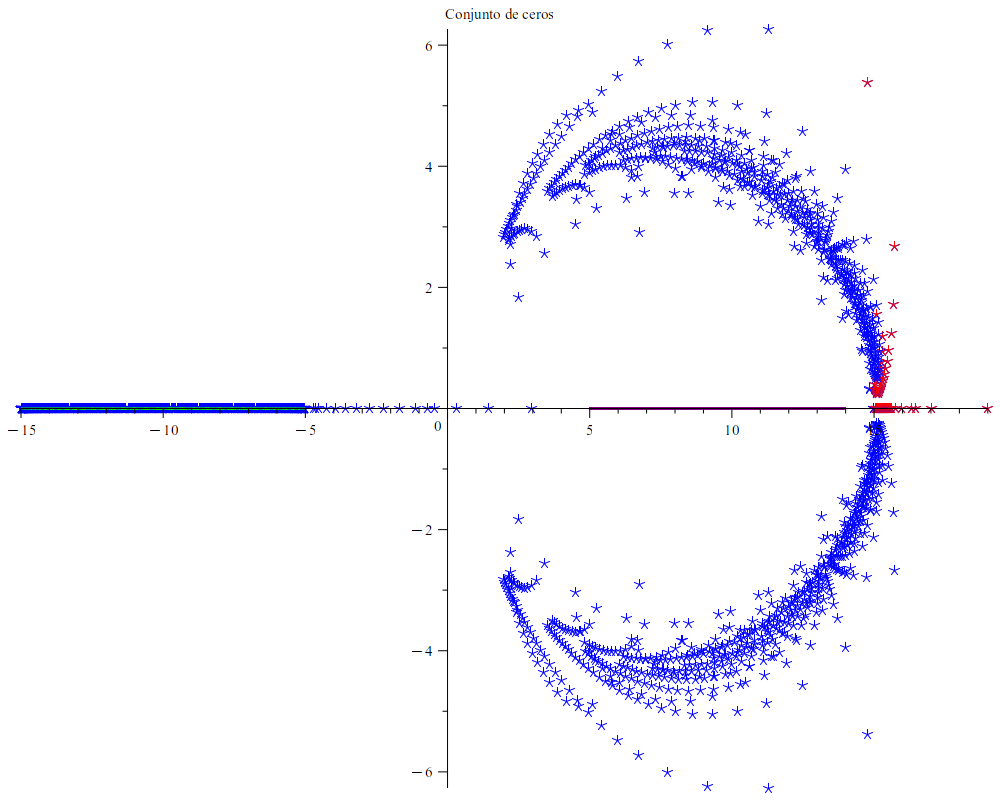
\includegraphics[width=0.9\textwidth]{include/a-15b-5c5d14_zeros.png}
\end{center}

\begin{enumerate}
	\item $\lim_{n \to 50}\sigma_{1,n}=2.338\times10^{11}$
	\item $\lim_{n \to 50} \rho(\mathcal{D}_{n})=15.094$
	\item $\max\{Z_{n}\}_{n=0}^{50}=19.007$
	\item $\lim_{n \to 50}\sigma_{2,n}=14.992$
\end{enumerate}

\textbf{Ejemplo 11.} $\langle p(t),q(t) \rangle = \int_{-1}^{1} p(t) q(t) \, dt + |p'(0)||q'(0)|.$

\begin{center}
	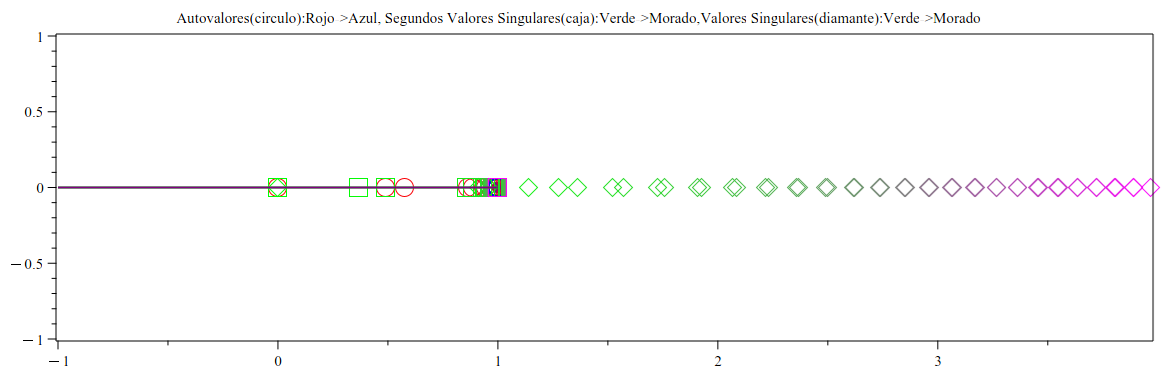
\includegraphics[width=0.9\textwidth]{include/a-1b1t0.png}

	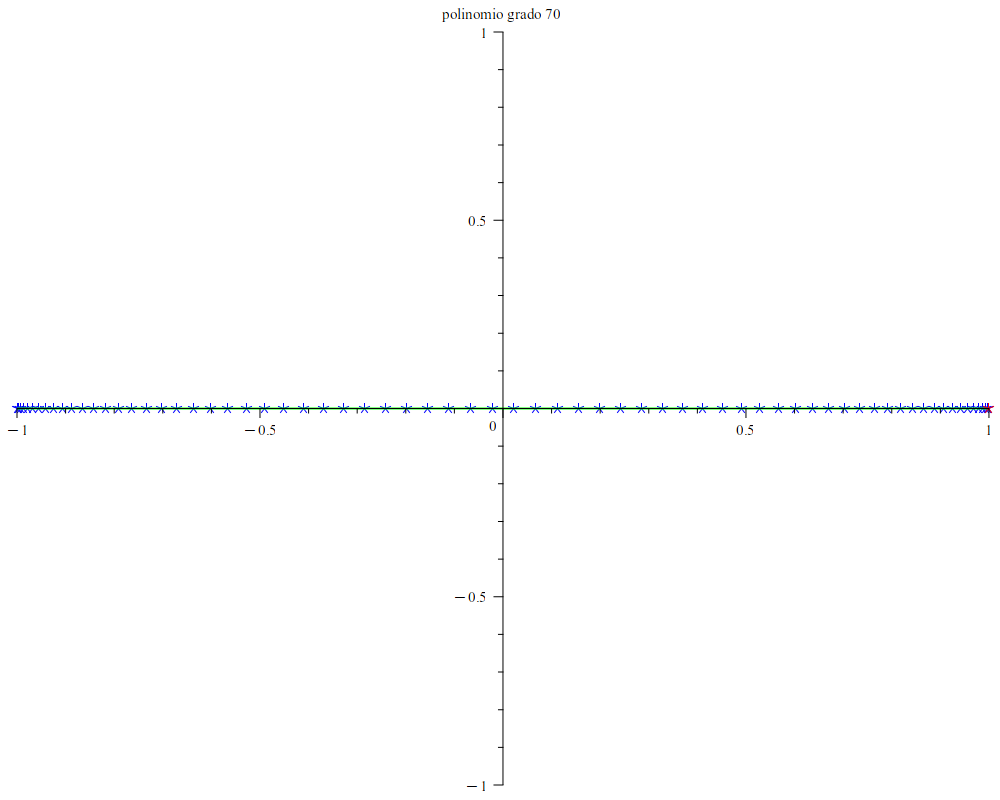
\includegraphics[width=0.9\textwidth]{include/a-1b1t0_zero.png}

	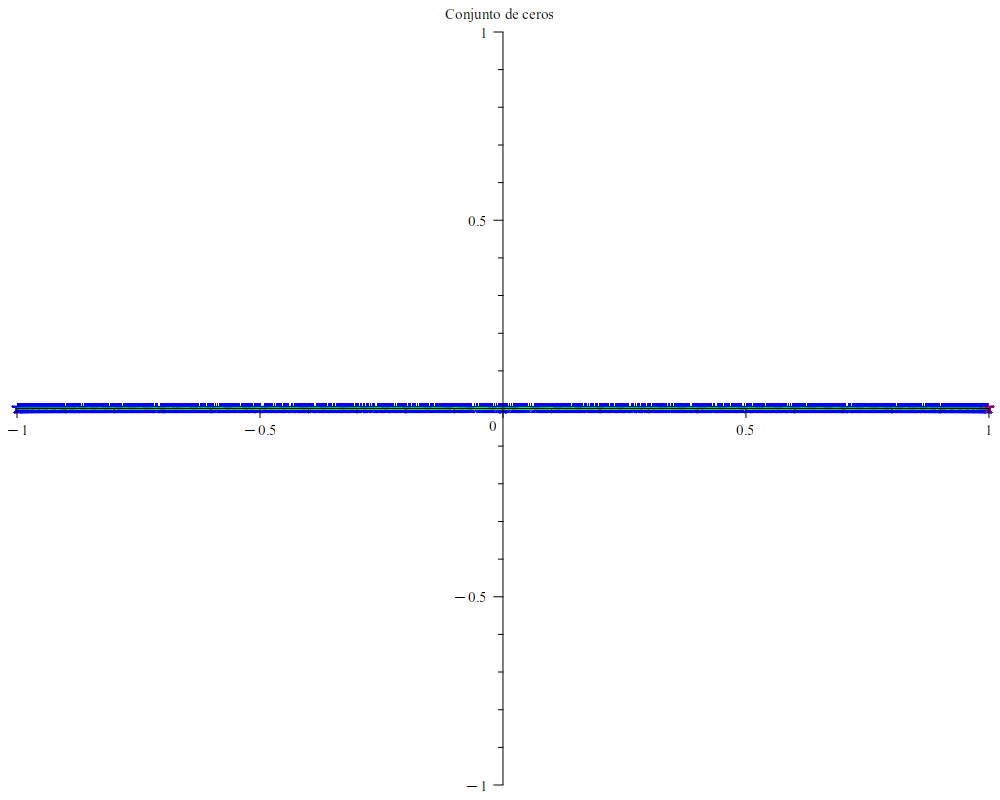
\includegraphics[width=0.9\textwidth]{include/a-1b1t0_zeros.png}
\end{center}

\begin{enumerate}
	\item $\lim_{n \to 50}\sigma_{1,n}=4.704$
	\item $\lim_{n \to 50} \rho(\mathcal{D}_{n})=0.999$
	\item $\max\{Z_{n}\}_{n=0}^{50}=0.999$
	\item $\lim_{n \to 50}\sigma_{2,n}=0.999$
\end{enumerate}

\textbf{Ejemplo 12.} $\langle p(t),q(t) \rangle = \int_{-1}^{1} p(t) q(t) \, dt + |p'(2)||q'(2)|.$

\begin{center}
	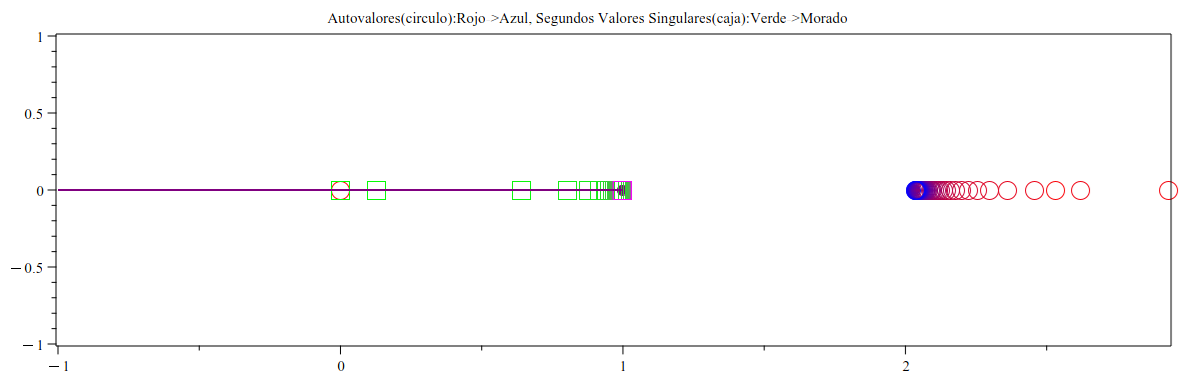
\includegraphics[width=0.9\textwidth]{include/a-1b1t2.png}

	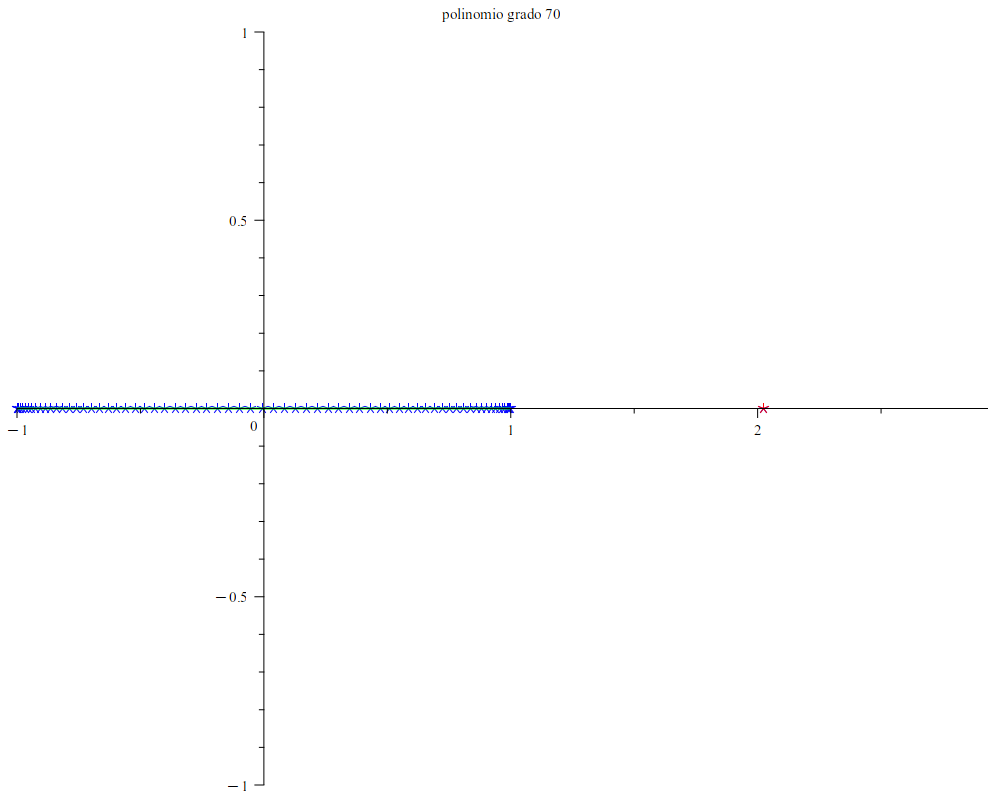
\includegraphics[width=0.9\textwidth]{include/a-1b1t2_zero.png}

	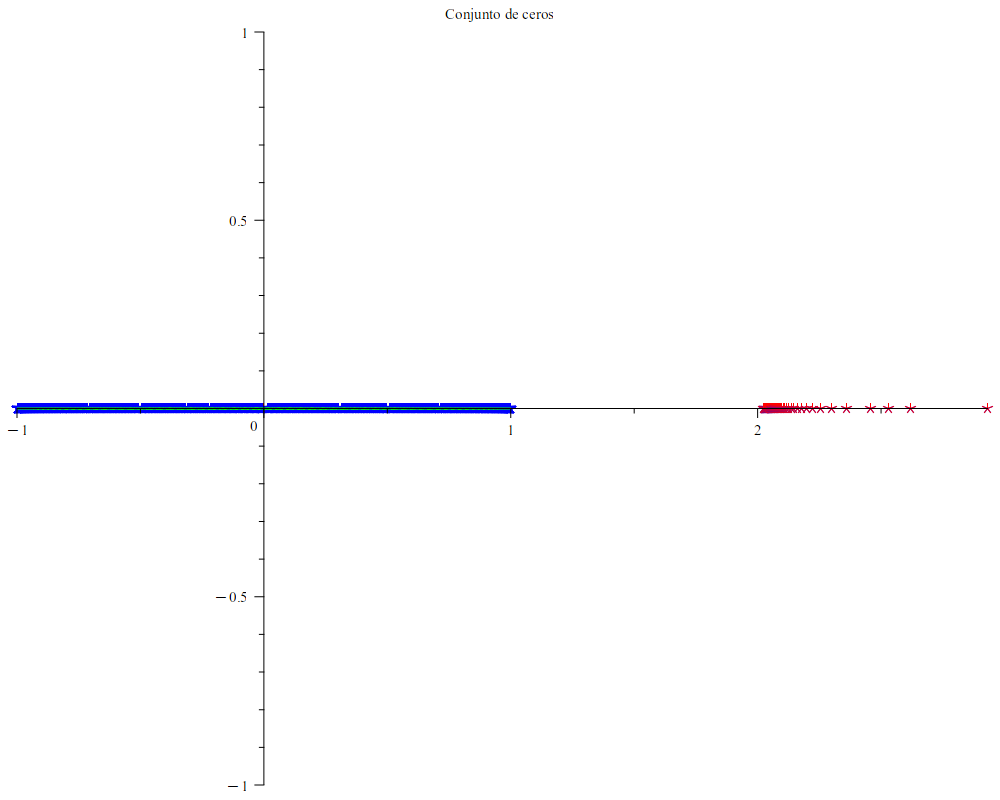
\includegraphics[width=0.9\textwidth]{include/a-1b1t2_zeros.png}
\end{center}

\begin{enumerate}
	\item $\lim_{n \to 50}\sigma_{1,n}=7.441\times10^{36}$
	\item $\lim_{n \to 50} \rho(\mathcal{D}_{n})=2.025$
	\item $\max\{Z_{n}\}_{n=0}^{50}=2.933$
	\item $\lim_{n \to 50}\sigma_{2,n}=0.999$
\end{enumerate}

\textbf{Ejemplo 13.} $\langle p(t),q(t) \rangle = \int_{0}^{1} p(t) q(t) \, dt + |p'(0)||q'(0)|.$

\begin{center}
	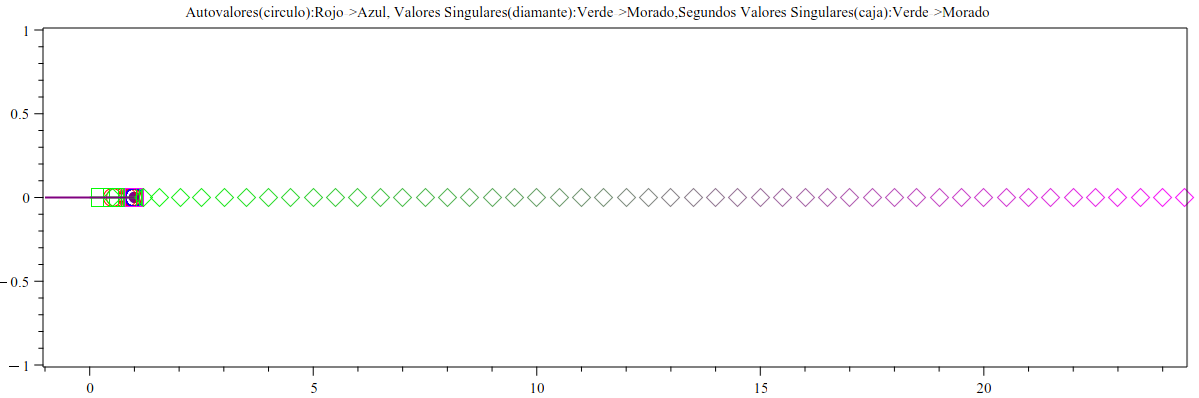
\includegraphics[width=0.9\textwidth]{include/a0b1t0.png}

	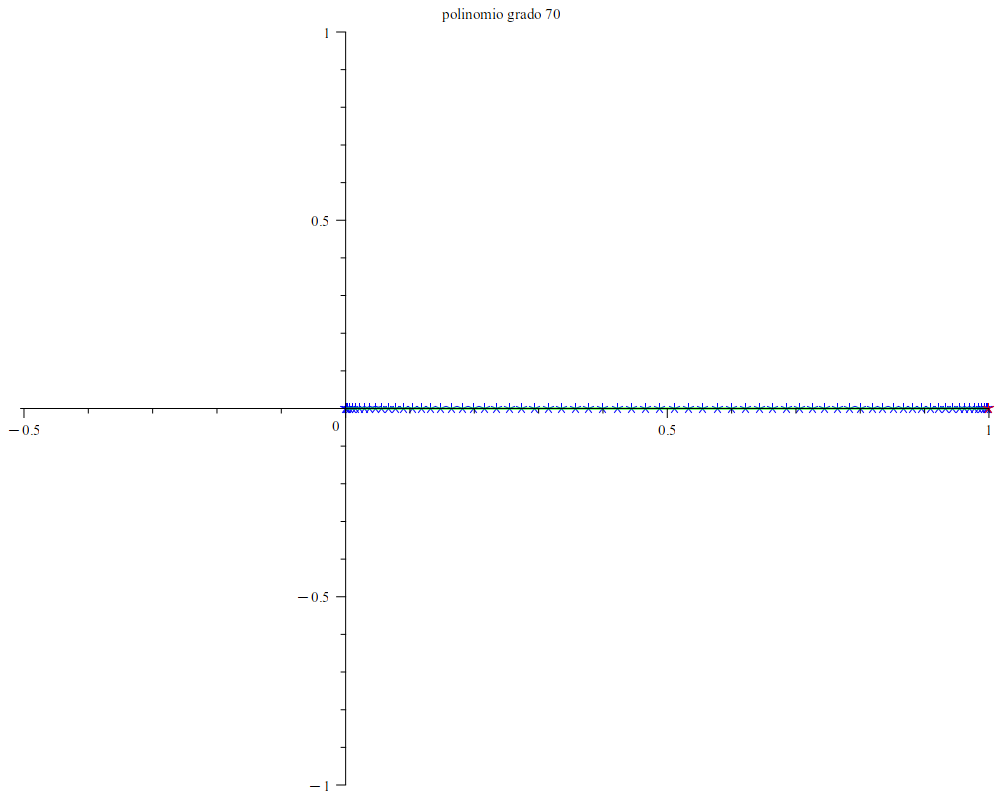
\includegraphics[width=0.9\textwidth]{include/a0b1t0_zero.png}

	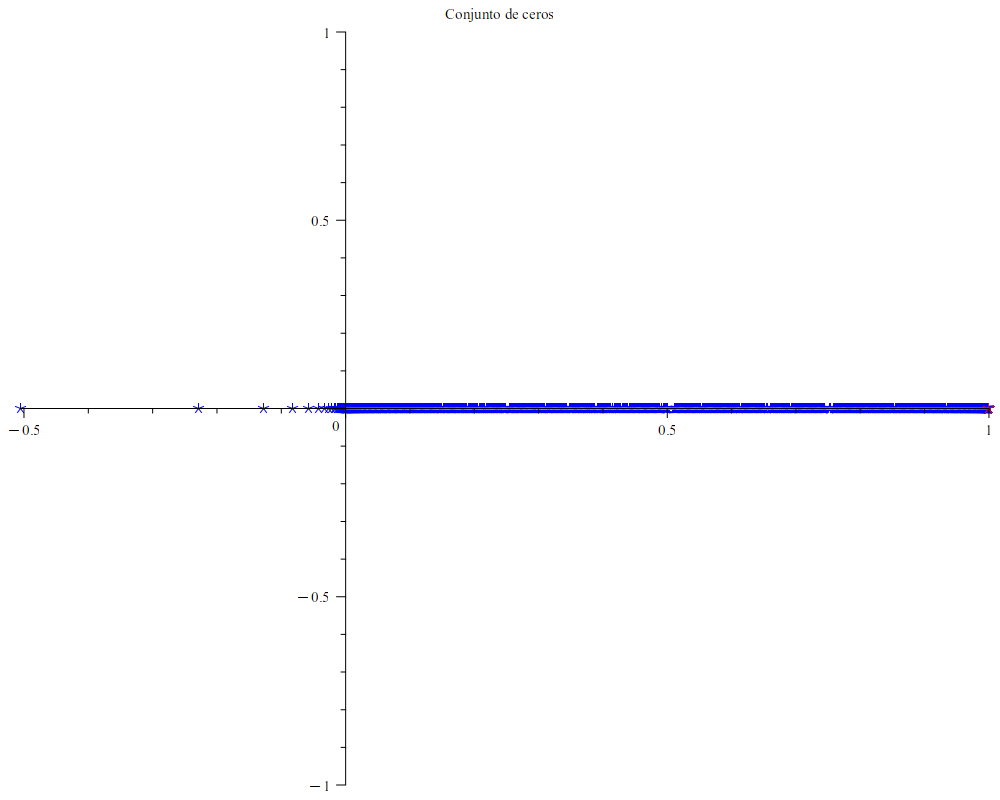
\includegraphics[width=0.9\textwidth]{include/a0b1t0_zeros.png}
\end{center}

\begin{enumerate}
	\item $\lim_{n \to 50}\sigma_{1,n}=35.000$
	\item $\lim_{n \to 50} \rho(\mathcal{D}_{n})=0.999$
	\item $\max\{Z_{n}\}_{n=0}^{50}=0.999$
	\item $\lim_{n \to 50}\sigma_{2,n}=0.999$
\end{enumerate}

\textbf{Ejemplo 14.} $\langle p(t),q(t) \rangle = \int_{0}^{1} p(t) q(t) \, dt + |p'(2)||q'(2)|.$

\begin{center}
	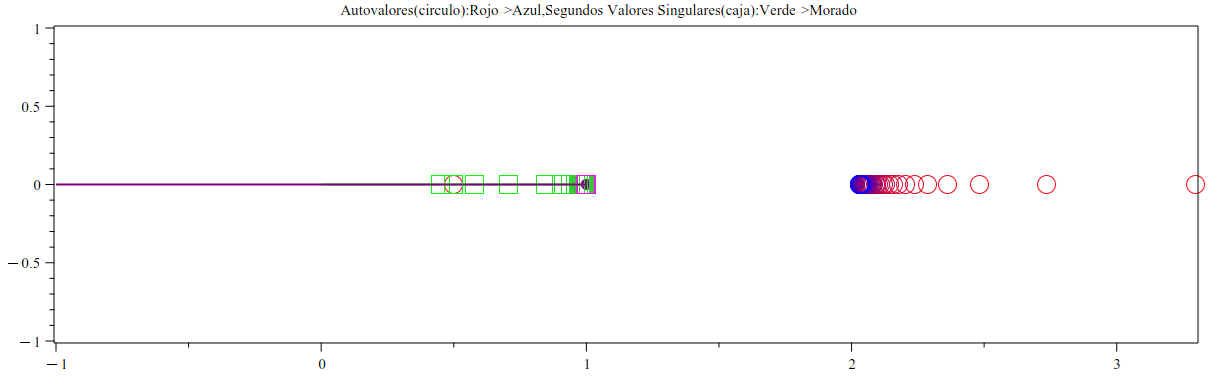
\includegraphics[width=0.9\textwidth]{include/a0b1t2.png}

	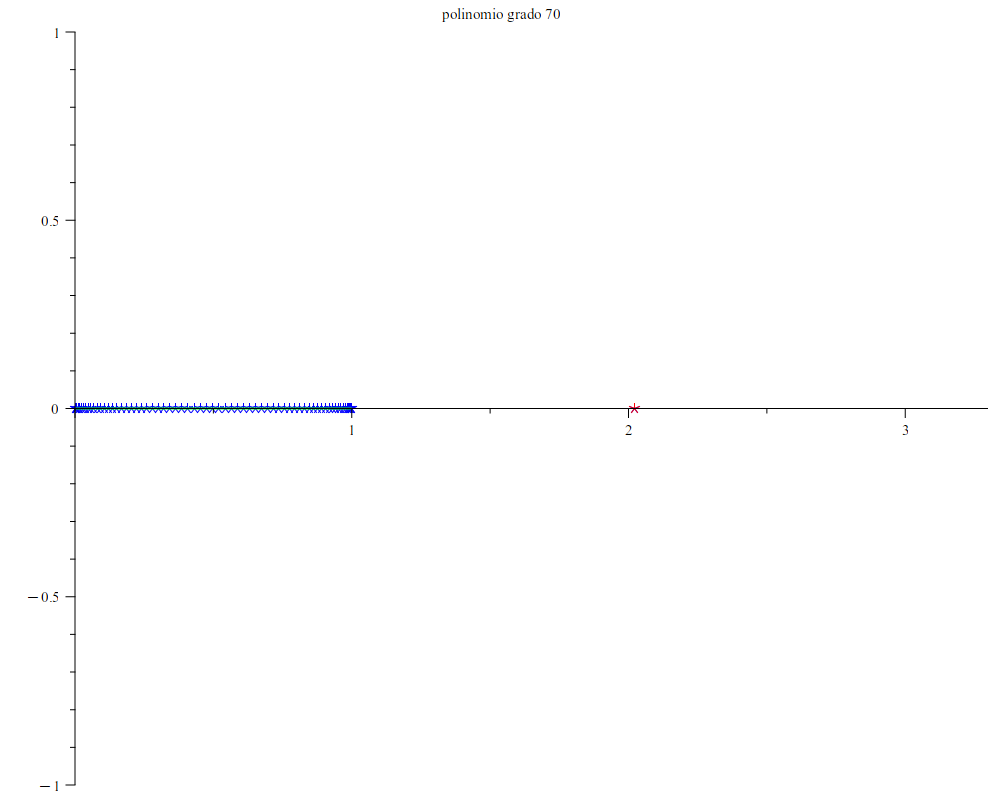
\includegraphics[width=0.9\textwidth]{include/a0b1t2_zero.png}

	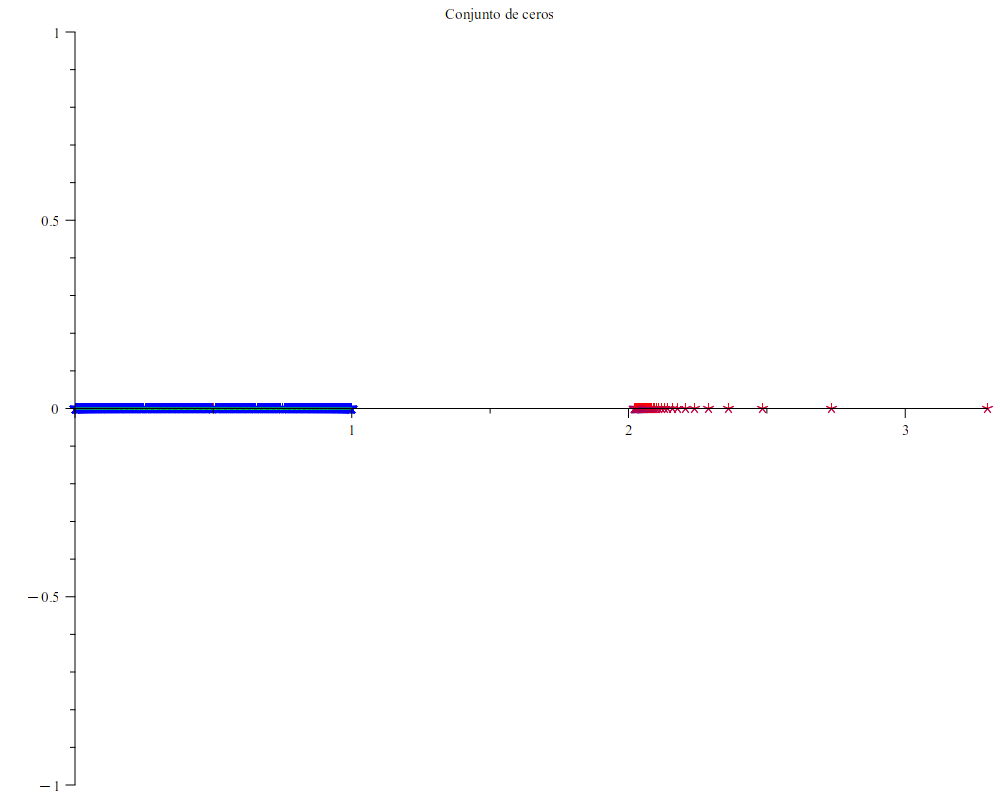
\includegraphics[width=0.9\textwidth]{include/a0b1t2_zeros.png}
\end{center}

\begin{enumerate}
	\item $\lim_{n \to 50}\sigma_{1,n}=1.405\times10^{50}$
	\item $\lim_{n \to 50} \rho(\mathcal{D}_{n})=2.021$
	\item $\max\{Z_{n}\}_{n=0}^{50}=3.299$
	\item $\lim_{n \to 50}\sigma_{2,n}=0.999$
\end{enumerate}

\begin{sidewaystable}
	\centering
	\small
	\caption{Resumen de ejemplos sobre la localización de ceros.}
	\begin{tabular}{|c|cccc|cccc|cccc|}
		\hline
		\multirow{3}{*}{\textbf{Parámetros}}       & \multicolumn{4}{c|}{\textbf{SECUENCIALMENTE}} & \multicolumn{4}{c|}{\textbf{NO SECUENCIALMENTE}} & \multicolumn{4}{c|}{\textbf{ÁTOMO}}                                                                                                                                                            \\
		                                           & \multicolumn{4}{c|}{\textbf{DOMINADO}}        & \multicolumn{4}{c|}{\textbf{DOMINADO}}           & \multicolumn{4}{c|}{}                                                                                                                                                                          \\
		\cline{2-13}
		                                           & $\sigma_{1,n}$                                & $\sigma_{2,n}$                                   & $\rho(\mathcal{D}_{n})$             & $\max Z$ & $\sigma_{1,n}$  & $\sigma_{2,n}$ & $\rho(\mathcal{D}_{n})$ & $\max Z$ & $\sigma_{1,n}$  & $\sigma_{2,n}$ & $\rho(\mathcal{D}_{n})$ & $\max Z$ \\
		\hline
		\textbf{Ej.1}: $[-1,1]t^2, [-1,1]t^{10}$   & 1.2760                                        & 1.2760                                           & 0.9999                              & 1.1333   & -               & -              & -                       & -        & -               & -              & -                       & -        \\
		\textbf{Ej.2}: $[-1,1]t^{10}, [-1,1]t^{2}$ & -                                             & -                                                & -                                   & -        & 2.2040          & 2.1220         & 1.0000                  & 1.2750   & -               & -              & -                       & -        \\
		\textbf{Ej.3}: $[0,10], [30,40]$           & -                                             & -                                                & -                                   & -        & $9.272×10^{16}$ & 39.9980        & 42.9300                 & 50.0520  & -               & -              & -                       & -        \\
		\textbf{Ej.4}: $[30,40], [0,10]$           & -                                             & -                                                & -                                   & -        & $9.272×10^{16}$ & 39.9910        & 39.9910                 & 39.9910  & -               & -              & -                       & -        \\
		\textbf{Ej.5}: $[0,10], [30,50]$           & -                                             & -                                                & -                                   & -        & $5.990×10^{13}$ & 49.9830        & 52.6560                 & 59.8140  & -               & -              & -                       & -        \\
		\textbf{Ej.6}: $[30,50], [0,10]$           & -                                             & -                                                & -                                   & -        & $3.752×10^{13}$ & 49.9870        & 49.9870                 & 49.9870  & -               & -              & -                       & -        \\
		\textbf{Ej.7}: $[0,20], [30,40]$           & -                                             & -                                                & -                                   & -        & $2.944×10^{9}$  & 39.9850        & 40.9510                 & 44.1960  & -               & -              & -                       & -        \\
		\textbf{Ej.8}: $[30,40], [0,20]$           & -                                             & -                                                & -                                   & -        & $4.136×10^{8}$  & 39.9890        & 39.9890                 & 39.9890  & -               & -              & -                       & -        \\
		\textbf{Ej.9}: $[-15,-5], [5,16]$          & -                                             & -                                                & -                                   & -        & $3.711×10^{10}$ & 15.9900        & 17.1070                 & 21.1520  & -               & -              & -                       & -        \\
		\textbf{Ej.10}: $[-15,-5], [5,14]$         & -                                             & -                                                & -                                   & -        & $2.338×10^{11}$ & 14.9920        & 15.0940                 & 19.0070  & -               & -              & -                       & -        \\
		\textbf{Ej.11}: $[-1,1], c=0$              & -                                             & -                                                & -                                   & -        & -               & -              & -                       & -        & 4.7040          & 0.9990         & 0.9990                  & 0.9990   \\
		\textbf{Ej.12}: $[-1,1], c=2$              & -                                             & -                                                & -                                   & -        & -               & -              & -                       & -        & $7.441×10^{36}$ & 0.9990         & 2.0250                  & 2.9330   \\
		\textbf{Ej.13}: $[0,1], c=0$               & -                                             & -                                                & -                                   & -        & -               & -              & -                       & -        & 35.0000         & 0.9990         & 0.9990                  & 0.9990   \\
		\textbf{Ej.14}: $[0,1], c=2$               & -                                             & -                                                & -                                   & -        & -               & -              & -                       & -        & $1.405×10^{50}$ & 0.9990         & 2.0210                  & 3.2990   \\
		\hline
	\end{tabular}
\end{sidewaystable}

\newpage

\section{Caso Circunferencia}

En este capítulo analizamos el comportamiento de los ceros de polinomios ortogonales de Sobolev en el caso complejo, donde las medidas están soportadas en circunferencias. Este enfoque nos permite extender nuestro estudio más allá del eje real y comprender mejor los fenómenos de distribución de ceros en el plano complejo.

% CASOS SECUENCIALMENTE DOMINADOS
\textbf{Ejemplo 1.} % Originalmente Ejemplo 1
$\langle p(z),q(z) \rangle=\int_{S_{0}(1)} p(z)\overline{q(z)}\, dm_{0;1} + \int_{S_{0.4}(0.4)} p'(z)\overline{q'(z)}\, dm_{0.4;0.4}$

\begin{center}
	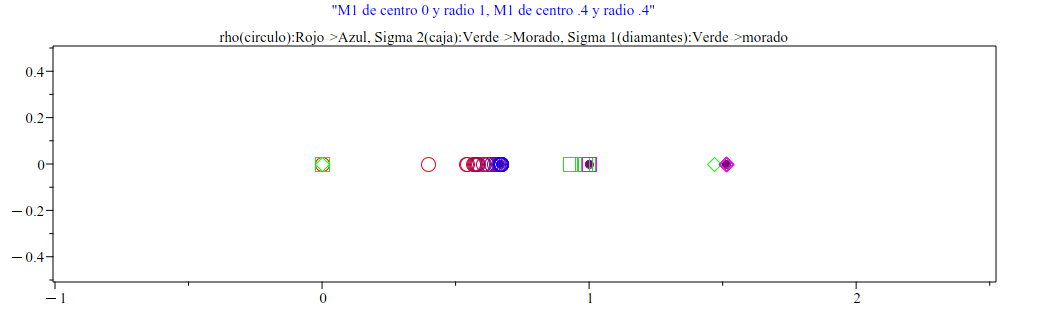
\includegraphics[width=0.9\textwidth]{include/r1_1c1_0r2_0.4c2_0.4.png}

	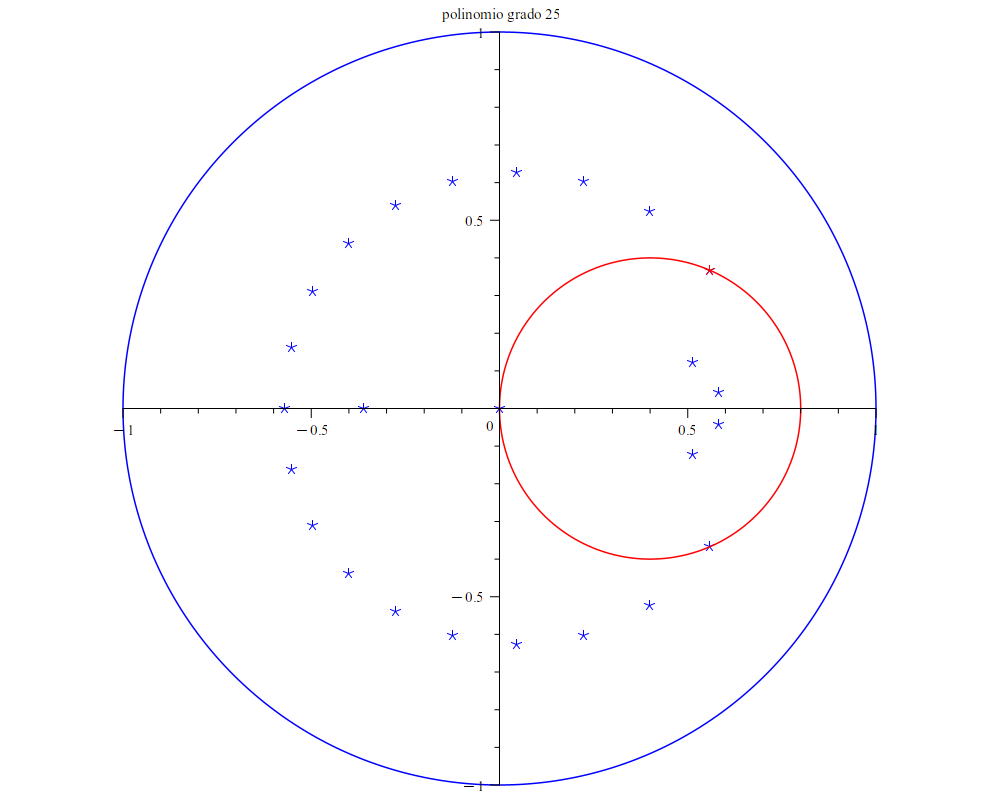
\includegraphics[width=0.9\textwidth]{include/r1_1c1_0r2_0.4c2_0.4_zero.png}

	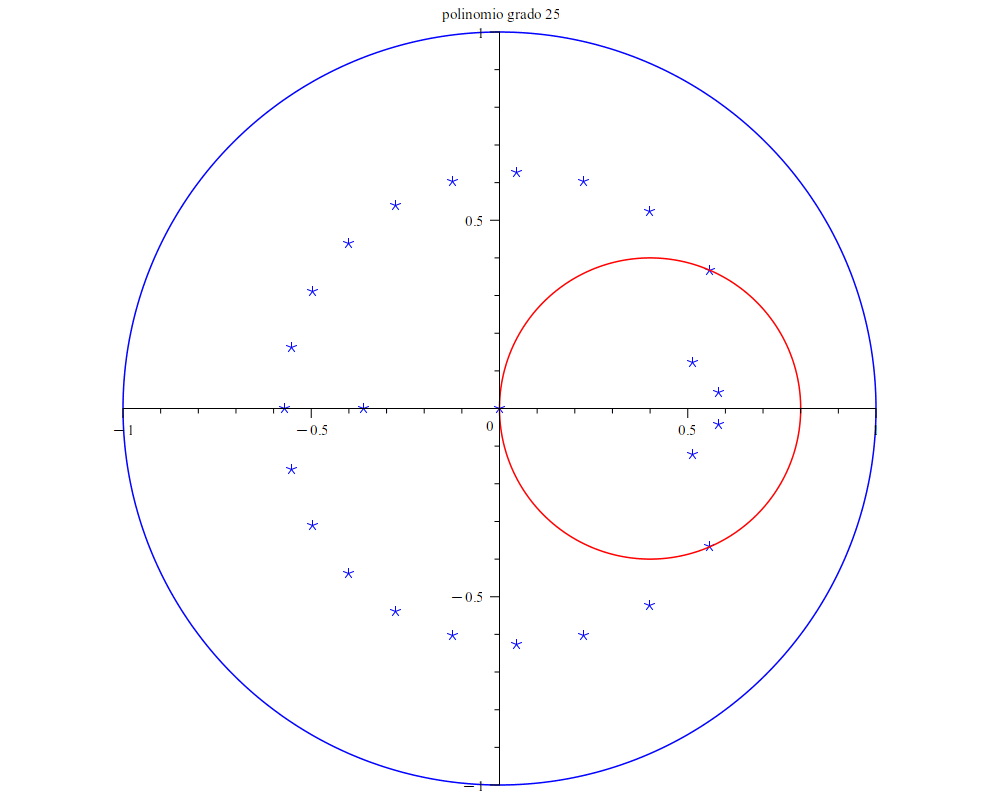
\includegraphics[width=0.9\textwidth]{include/r1_1c1_0r2_0.4c2_0.4_zeros.png}
\end{center}

\begin{enumerate}
	\item $\lim_{n \to 25}\sigma_{1,n}=1.516$
	\item $\lim_{n \to 25} \rho(\mathcal{D}_{n})=0.667$
	\item $\max\{Z_{n}\}_{n=0}^{25}=0.672$
	\item $\lim_{n \to 25}\sigma_{2,n}=1.000$
\end{enumerate}

\textbf{Ejemplo 2.} % Originalmente Ejemplo 3
$\langle p(z),q(z) \rangle=\int_{S_{0}(1)} p(z)\overline{q(z)}\, dm_{0;1} + \int_{S_{0.5}(2)} p'(z)\overline{q'(z)}\, dm_{0.5;2}$

\begin{center}
	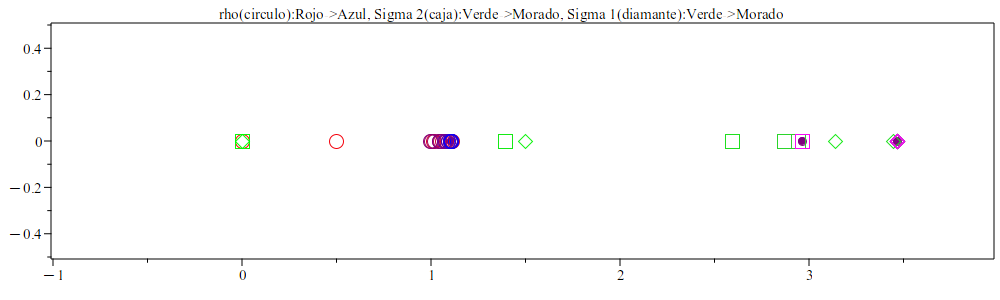
\includegraphics[width=0.9\textwidth]{include/r1_1c1_0r2_2c2_0.5.png}

	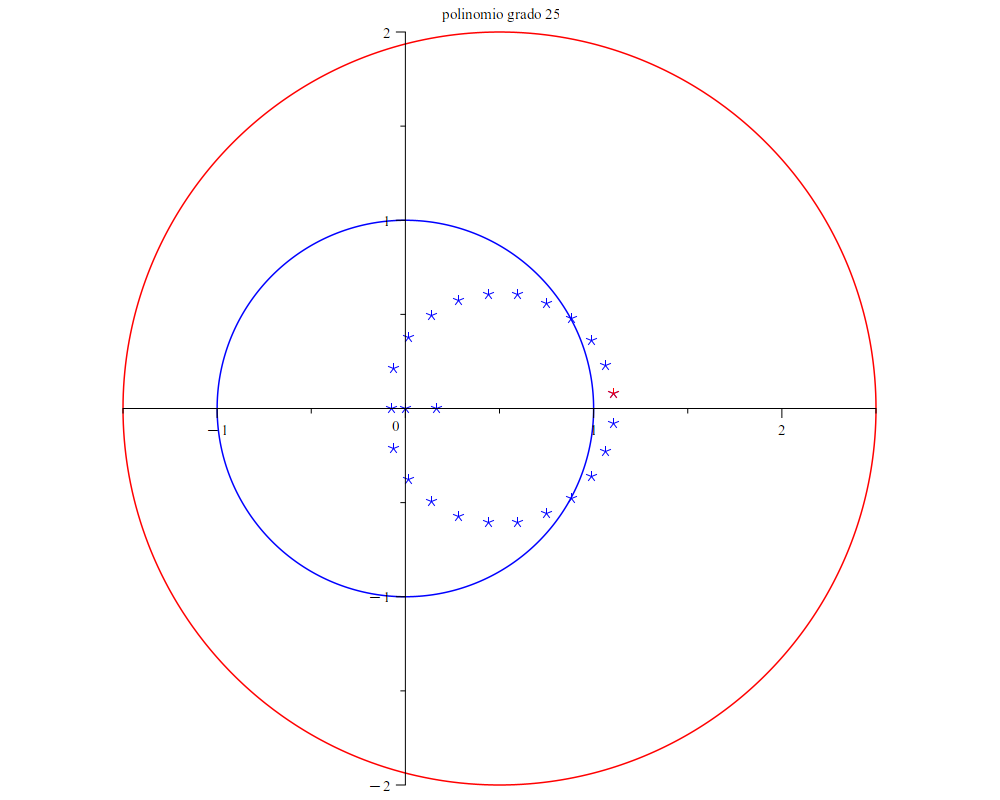
\includegraphics[width=0.9\textwidth]{include/r1_1c1_0r2_2c2_0.5_zero.png}

	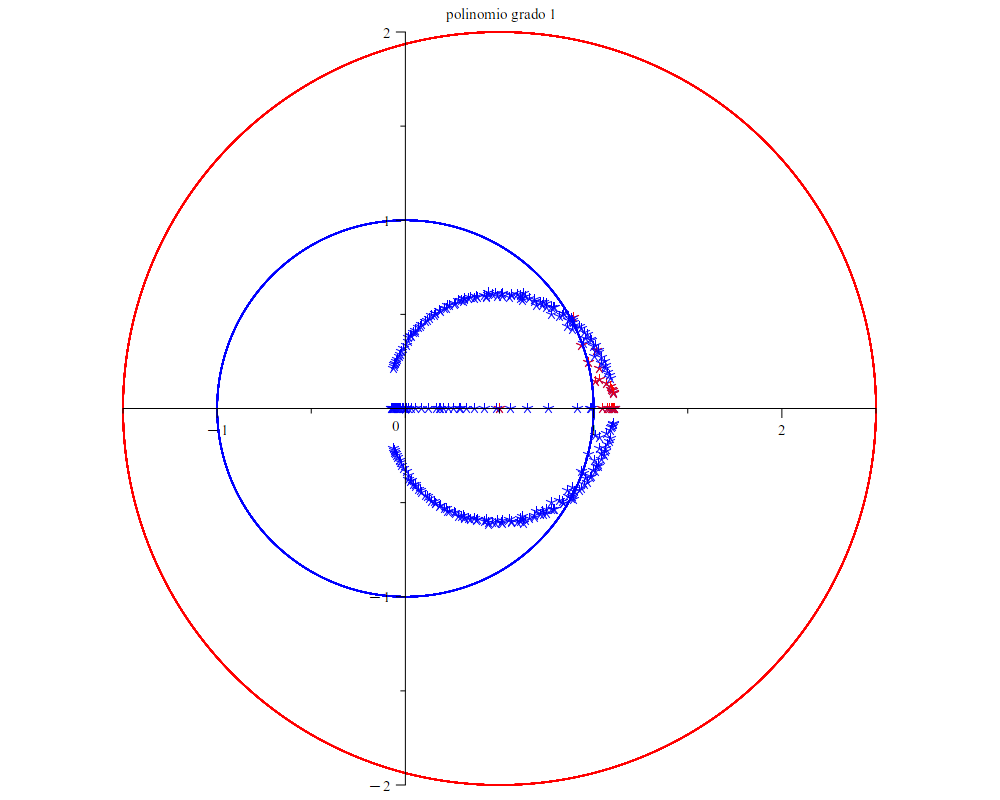
\includegraphics[width=0.9\textwidth]{include/r1_1c1_0r2_2c2_0.5_zeros.png}
\end{center}

\begin{enumerate}
	\item $\lim_{n \to 25}\sigma_{1,n}=3.470$
	\item $\lim_{n \to 25} \rho(\mathcal{D}_{n})=1.108$
	\item $\max\{Z_{n}\}_{n=0}^{25}=1.112$
	\item $\lim_{n \to 25}\sigma_{2,n}=2.968$
\end{enumerate}

\textbf{Ejemplo 3.} % Originalmente Ejemplo 3
$\langle p(z),q(z) \rangle=\int_{S_{0}(1)} p(z)\overline{q(z)}\, dm_{0;1} + \int_{S_{0.5}(10)} p'(z)\overline{q'(z)}\, dm_{0.5;10}$

\begin{center}
	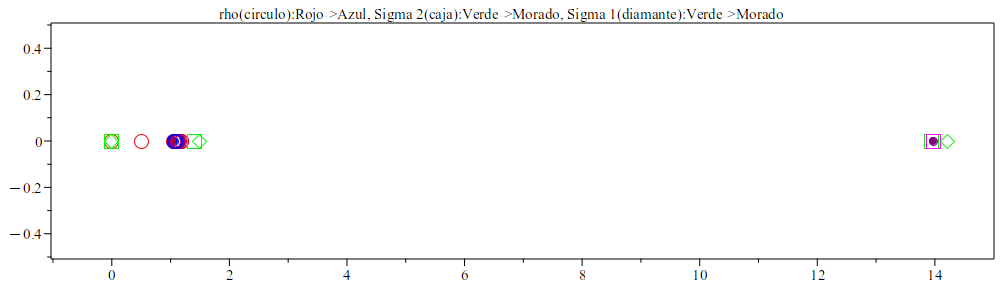
\includegraphics[width=0.9\textwidth]{include/r1_1c1_0r2_10c2_0.5.png}

	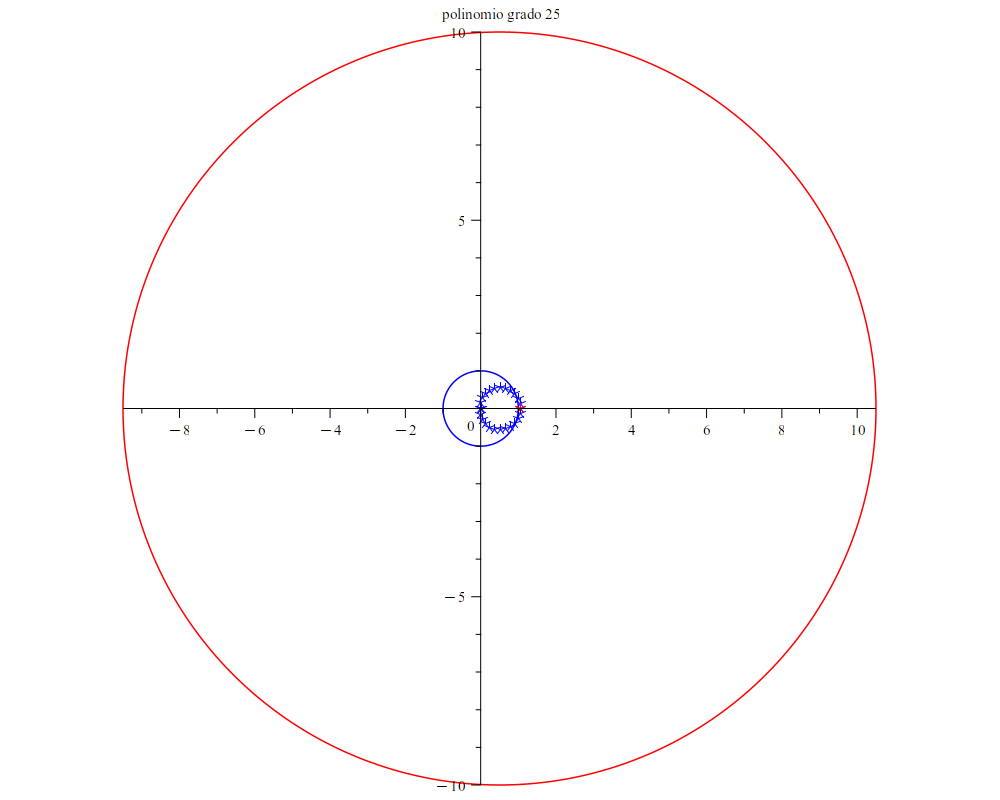
\includegraphics[width=0.9\textwidth]{include/r1_1c1_0r2_10c2_0.5_zero.png}

	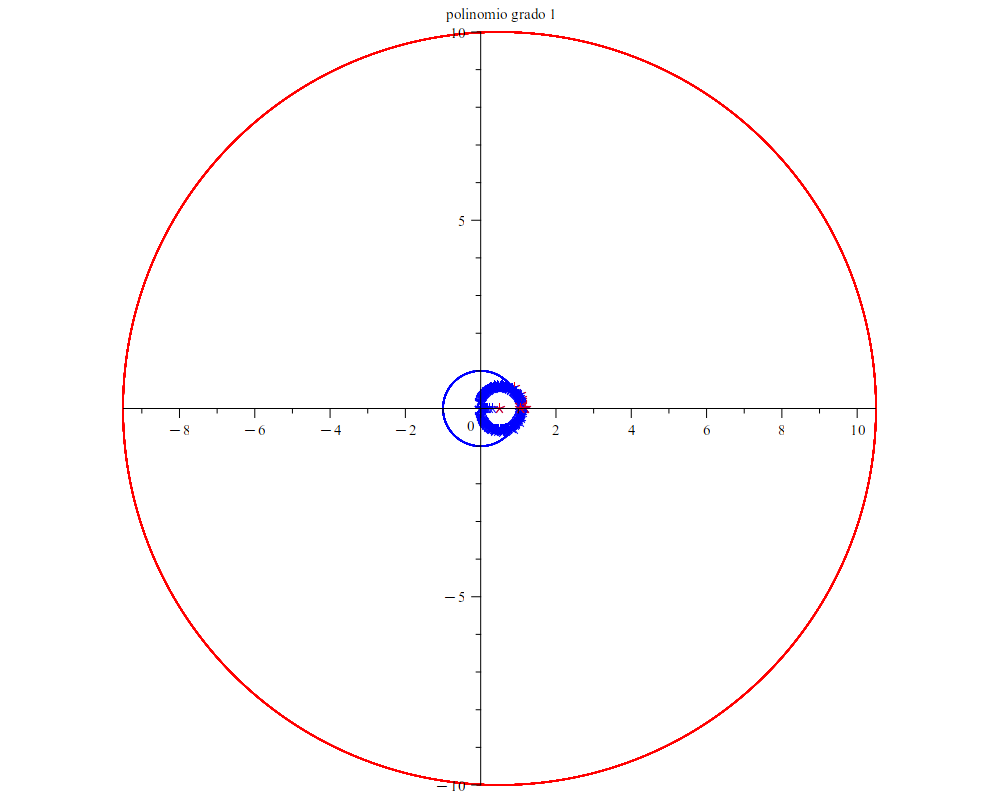
\includegraphics[width=0.9\textwidth]{include/r1_1c1_0r2_10c2_0.5_zeros.png}
\end{center}

\begin{enumerate}
	\item $\lim_{n \to 25}\sigma_{1,n}=15.248$
	\item $\lim_{n \to 25} \rho(\mathcal{D}_{n})=1.068$
	\item $\max\{Z_{n}\}_{n=0}^{25}=1.185$
	\item $\lim_{n \to 25}\sigma_{2,n}=13.972$
\end{enumerate}

% CASOS NO SECUENCIALMENTE DOMINADOS
\textbf{Ejemplo 4.} % Originalmente Ejemplo 2
$\langle p(z),q(z) \rangle=\int_{S_{0}(1)} p(z)\overline{q(z)}\, dm_{0;1} + \int_{S_{1}(1)} p'(z)\overline{q'(z)}\, dm_{1;1}$

\begin{center}
	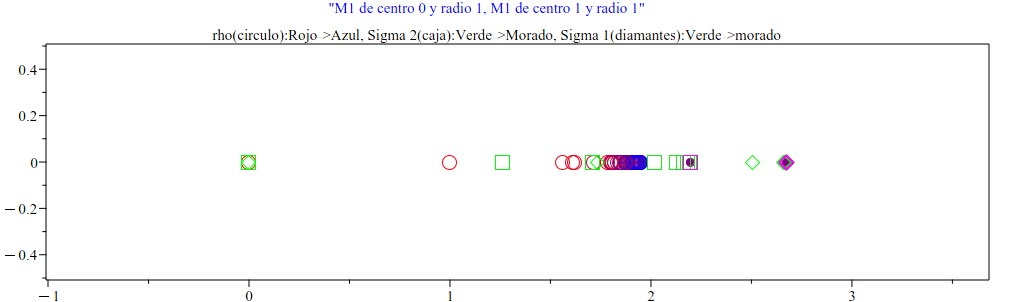
\includegraphics[width=0.9\textwidth]{include/r1_1c1_0r2_1c2_1.png}

	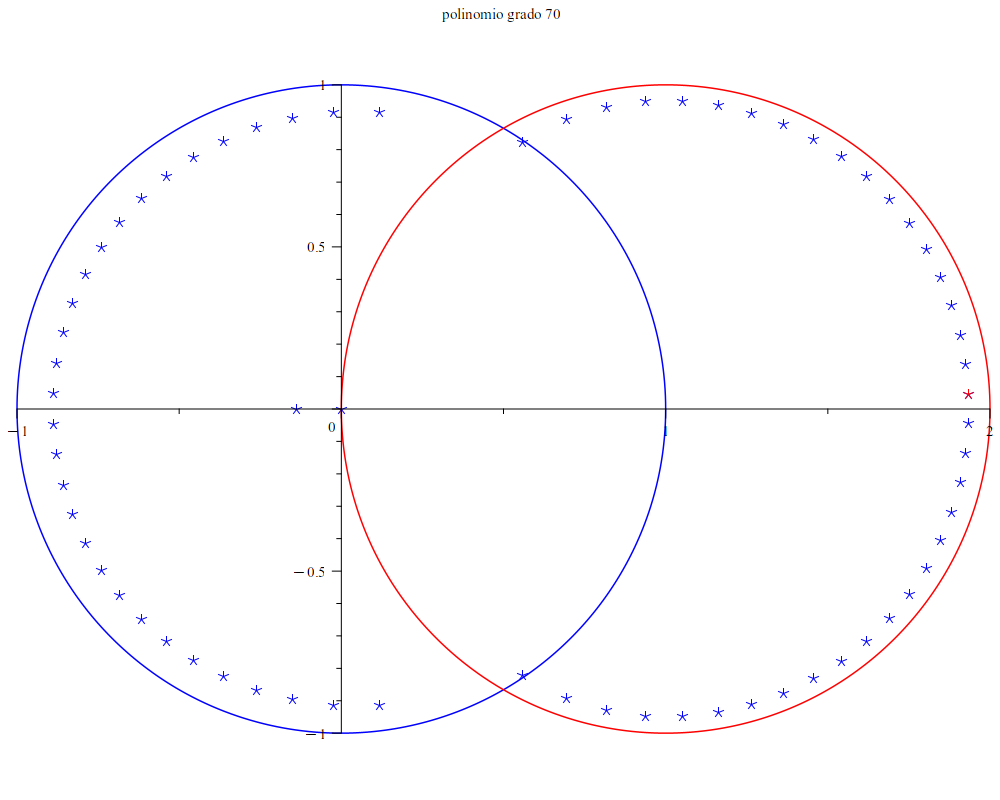
\includegraphics[width=0.9\textwidth]{include/r1_1c1_0r2_1c2_1_zero.png}

	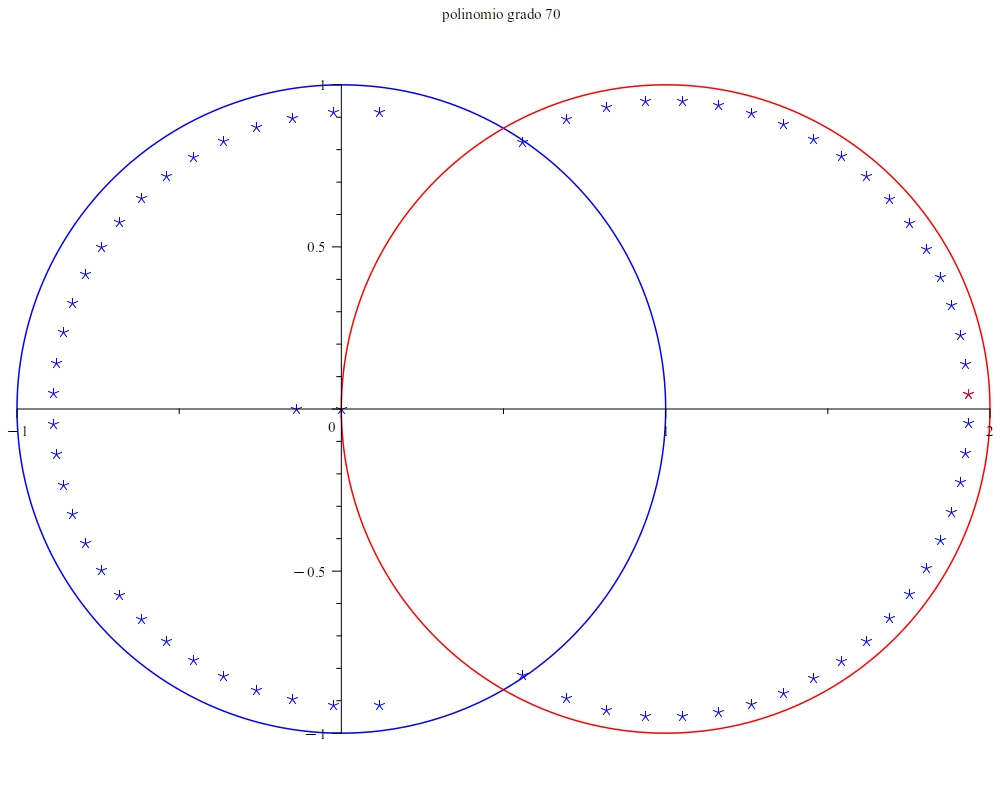
\includegraphics[width=0.9\textwidth]{include/r1_1c1_0r2_1c2_1_zeros.png}
\end{center}

\begin{enumerate}
	\item $\lim_{n \to 70}\sigma_{1,n}=2.672$
	\item $\lim_{n \to 70} \rho(\mathcal{D}_{n})=1.933$
	\item $\max\{Z_{n}\}_{n=0}^{70}=1.963$
	\item $\lim_{n \to 70}\sigma_{2,n}=2.672$
\end{enumerate}

\textbf{Ejemplo 5.} % Originalmente Ejemplo 4
$\langle p(z),q(z) \rangle=\int_{S_{0}(1)} p(z)\overline{q(z)}\, dm_{0;1} + \int_{S_{-10}(1)} p'(z)\overline{q'(z)}\, dm_{-10;1}$

\begin{center}
	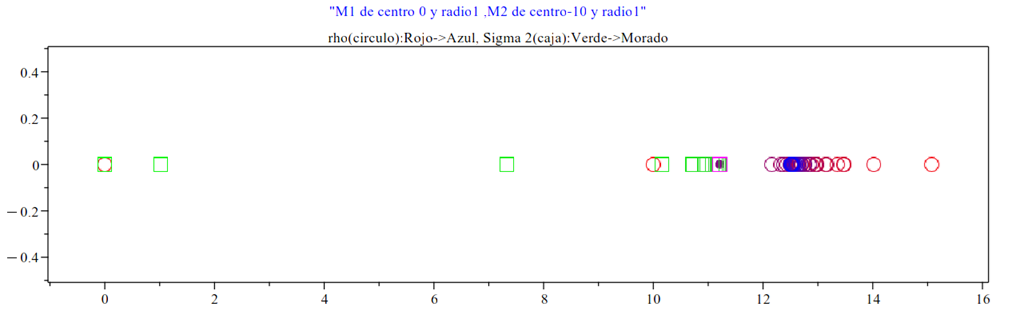
\includegraphics[width=0.9\textwidth]{include/r1_1c1_0r2_1c2_-10.png}

	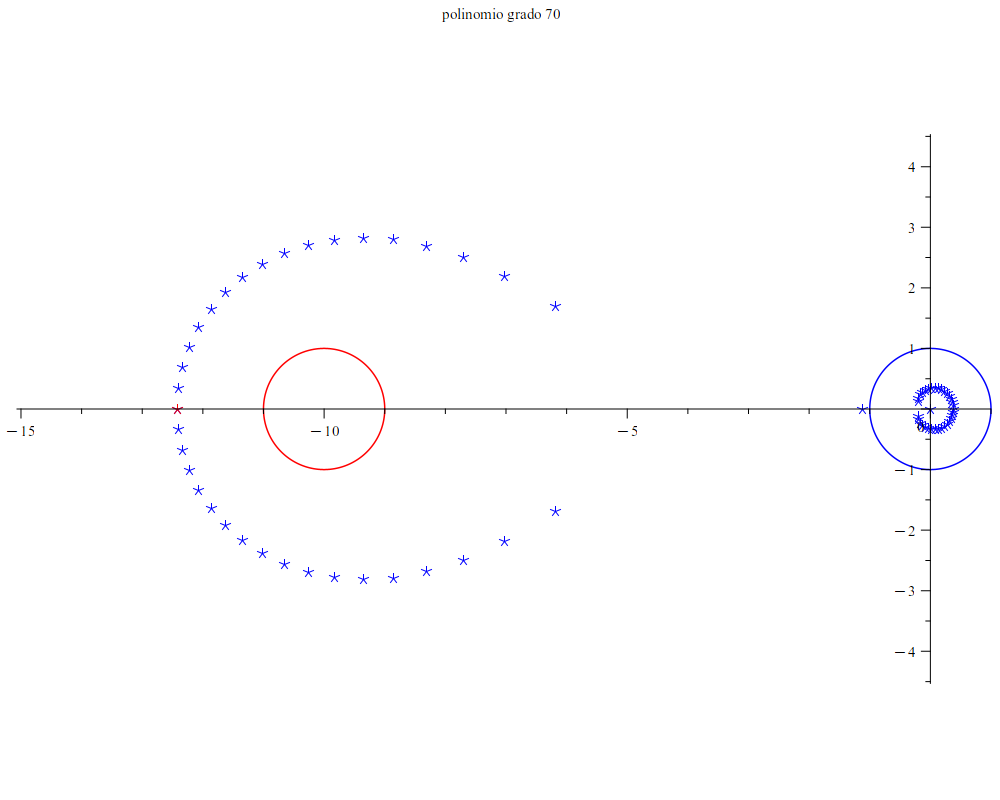
\includegraphics[width=0.9\textwidth]{include/r1_1c1_0r2_1c2_-10_zero.png}

	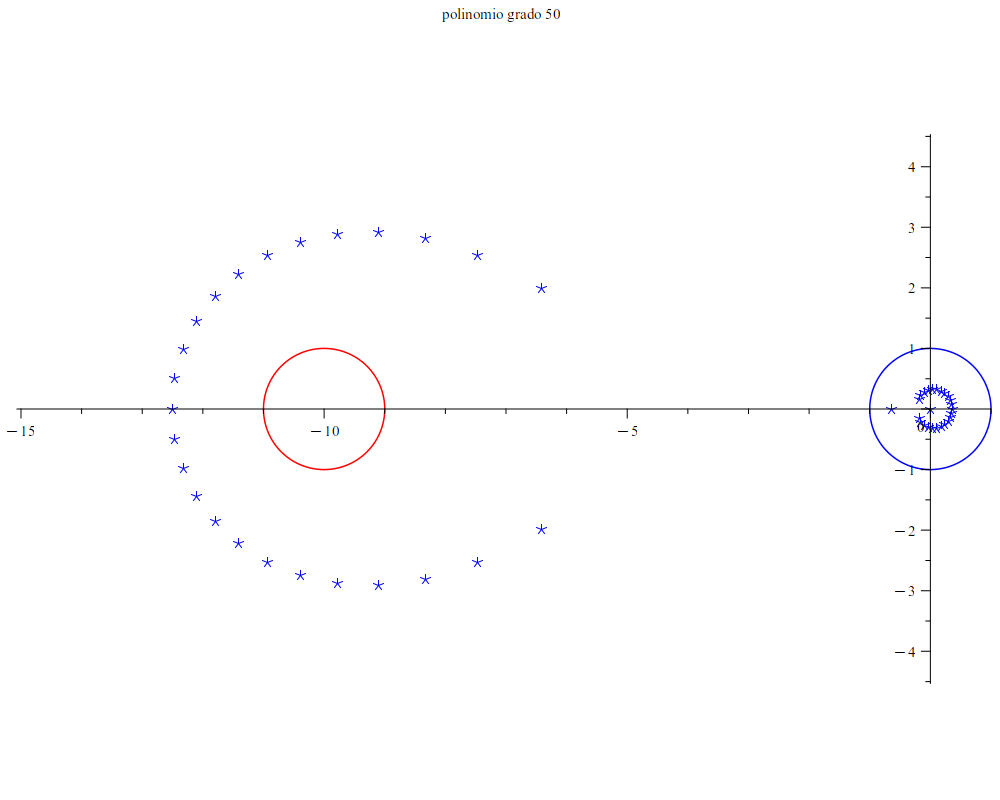
\includegraphics[width=0.9\textwidth]{include/r1_1c1_0r2_1c2_-10_zeros.png}
\end{center}

\begin{enumerate}
	\item $\lim_{n \to 70}\sigma_{1,n}=4.963 \times 10^{14}$
	\item $\lim_{n \to 70} \rho(\mathcal{D}_{n})=12.424$
	\item $\max\{Z_{n}\}_{n=0}^{70}=15.074$
	\item $\lim_{n \to 70}\sigma_{2,n}=11.211$
\end{enumerate}

\textbf{Ejemplo 6.} % Originalmente Ejemplo 6
$\langle p(z),q(z) \rangle=\int_{S_{-10}(0.25)} p(z)\overline{q(z)}\, dm_{-10;0.25} + \int_{S_{0}(1)} p'(z)\overline{q'(z)}\, dm_{0;1}$

\begin{center}
	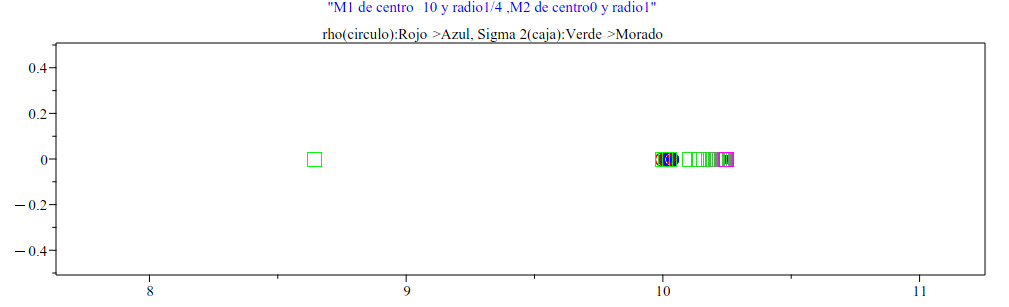
\includegraphics[width=0.9\textwidth]{include/r1_0.25c1_-10r2_1c2_0.png}

	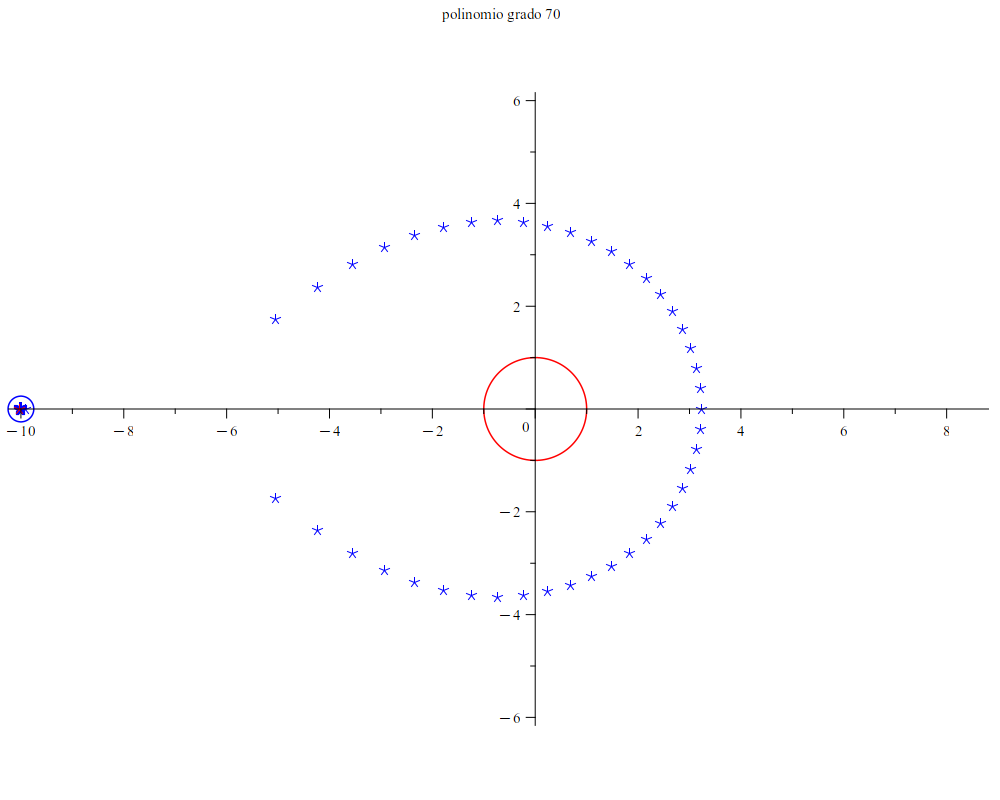
\includegraphics[width=0.9\textwidth]{include/r1_0.25c1_-10r2_1c2_0_zero.png}

	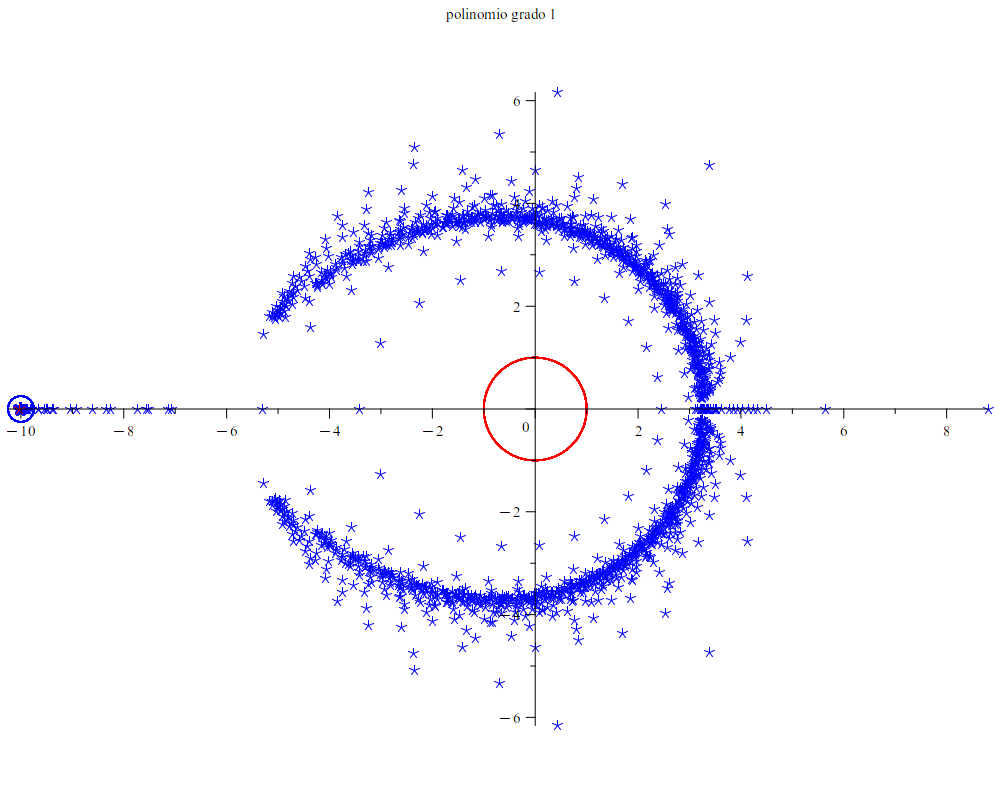
\includegraphics[width=0.9\textwidth]{include/r1_0.25c1_-10r2_1c2_0_zeros.png}
\end{center}

\begin{enumerate}
	\item $\lim_{n \to 70}\sigma_{1,n}=9.660 \times 10^{22}$
	\item $\lim_{n \to 70} \rho(\mathcal{D}_{n})=10.035$
	\item $\max\{Z_{n}\}_{n=0}^{70}=10.035$
	\item $\lim_{n \to 70}\sigma_{2,n}=10.249$
\end{enumerate}

\textbf{Ejemplo 7.} % Nuevo ejemplo
$\langle p(z),q(z) \rangle=\int_{S_{0}(1)} p(z)\overline{q(z)}\, dm_{0;1} + \int_{S_{-10}(0.25)} p'(z)\overline{q'(z)}\, dm_{-10;0.25}$

\begin{center}
	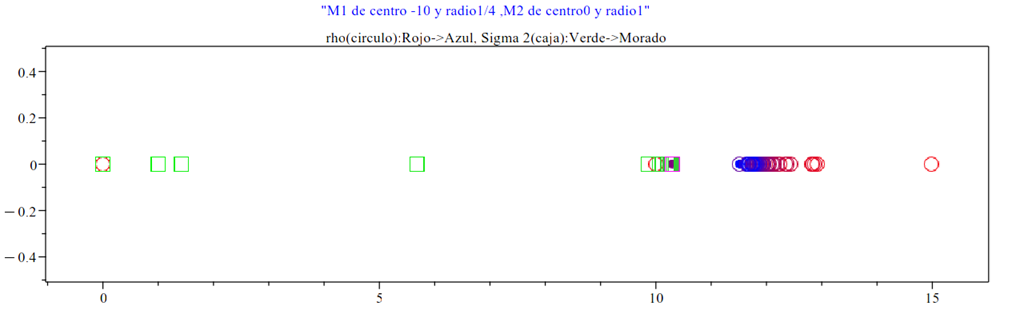
\includegraphics[width=0.9\textwidth]{include/r1_1c1_0r2_0.25c2_-10.png}

	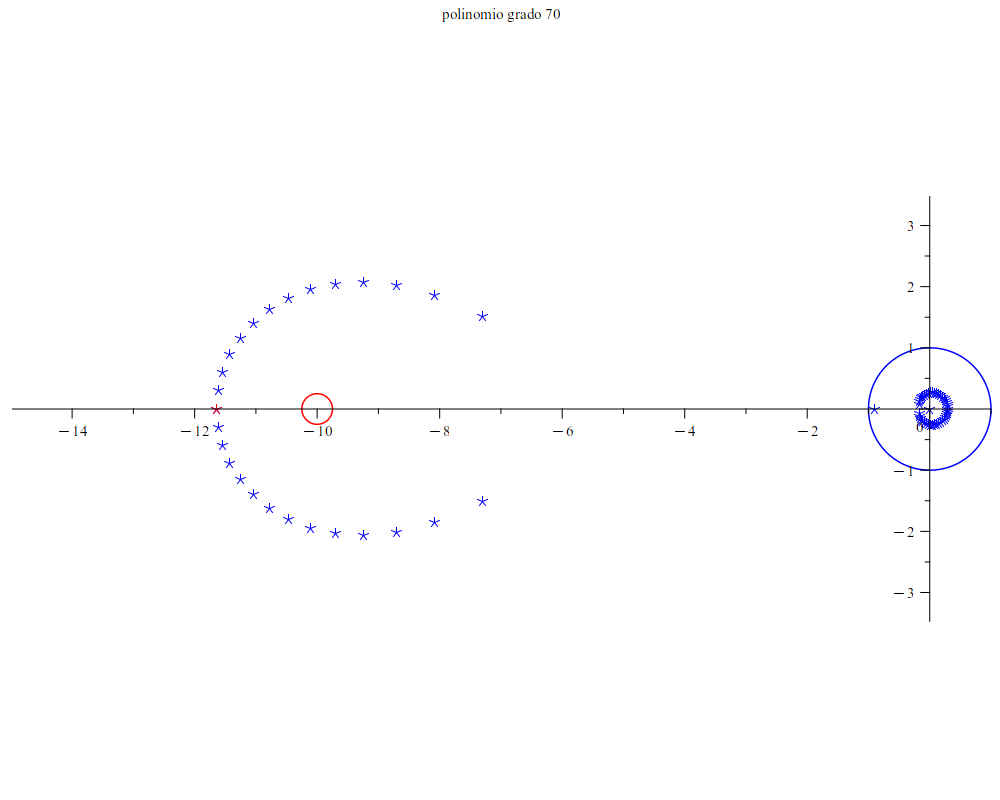
\includegraphics[width=0.9\textwidth]{include/r1_1c1_0r2_0.25c2_-10_zero.png}

	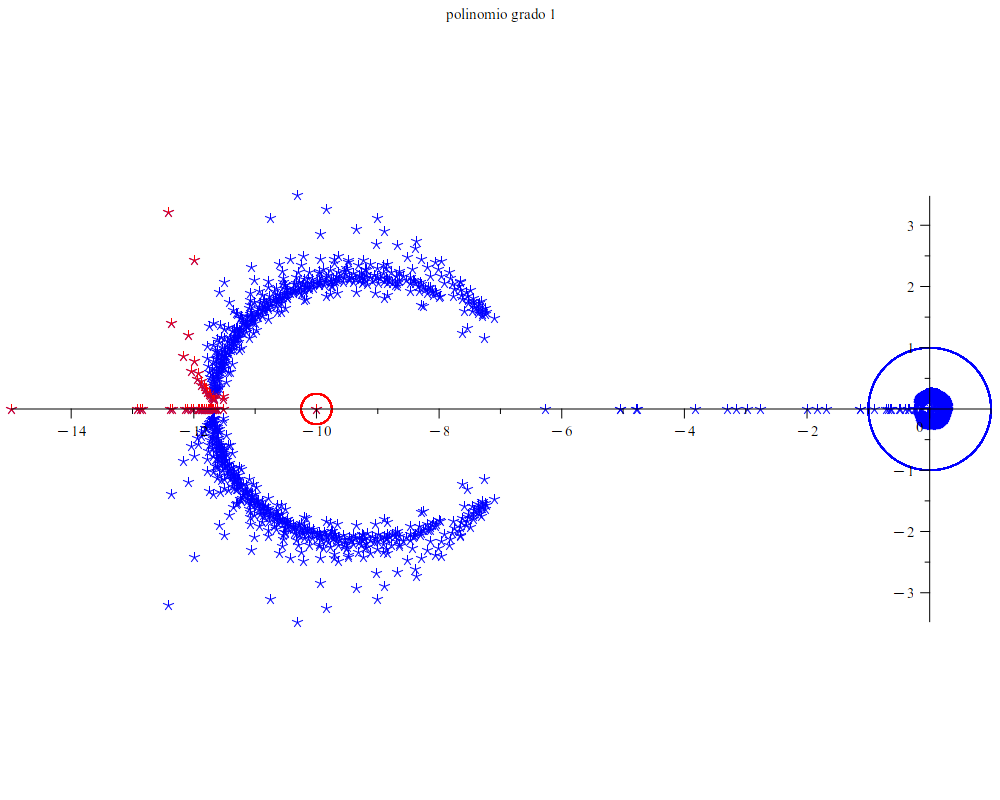
\includegraphics[width=0.9\textwidth]{include/r1_1c1_0r2_0.25c2_-10_zeros.png}
\end{center}

\begin{enumerate}
	\item $\lim_{n \to 50}\sigma_{1,n}=1.409 \times 10^{23}$
	\item $\lim_{n \to 50} \rho(\mathcal{D}_{n})=11.641$
	\item $\max\{Z_{n}\}_{n=0}^{50}=14.981$
	\item $\lim_{n \to 50}\sigma_{2,n}=10.2977$
\end{enumerate}

% CASOS CON ÁTOMO
\textbf{Ejemplo 8.} % Originalmente Ejemplo 5
$\langle p(z),q(z) \rangle=\int_{S_{0}(1)} p(z)\overline{q(z)}\, dm_{0;1} + p'(0.5+0.5i)\overline{q'(0.5+0.5i)}$

\begin{center}
	\begin{minipage}{0.48\textwidth}
		\centering
		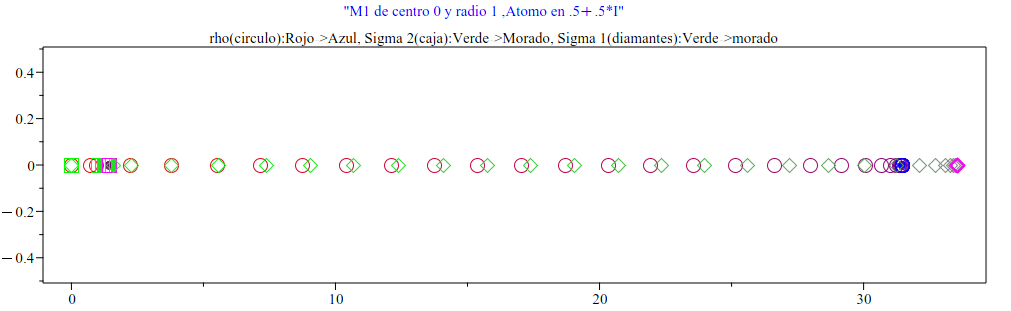
\includegraphics[width=\textwidth]{include/r1_1c1_0c2_(0.5)(0.5).png}
	\end{minipage}%
	\hfill
	\begin{minipage}{0.48\textwidth}
		\centering
		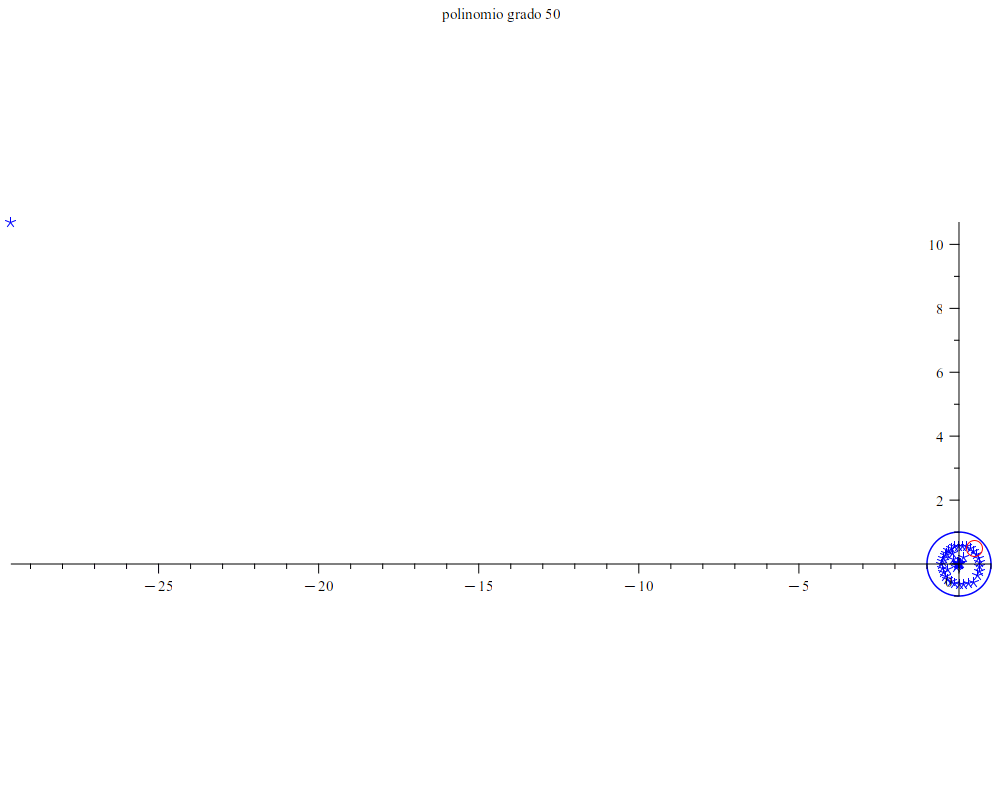
\includegraphics[width=\textwidth]{include/r1_1c1_0c2_(0.5)(0.5)_zeros.png}
	\end{minipage}
\end{center}

\begin{enumerate}
	\item $\lim_{n \to 50}\sigma_{1,n}=33.5602$
	\item $\lim_{n \to 50} \rho(\mathcal{D}_{n})=31.4890$
	\item $\max\{Z_{n}\}_{n=0}^{50}=31.4890$
	\item $\lim_{n \to 50}\sigma_{2,n}=1.4573$
\end{enumerate}

\textbf{Ejemplo 9.} % Originalmente Ejemplo 5
$\langle p(z),q(z) \rangle=\int_{S_{-0.5-0.5i}(1)} p(z)\overline{q(z)}\, dm_{-0.5-0.5i;1} + p'(0)\overline{q'(0)}$

\begin{center}
	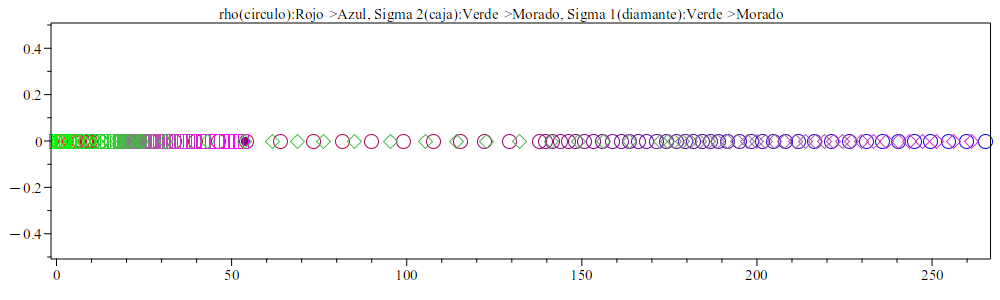
\includegraphics[width=0.9\textwidth]{include/r1_1c1_(-0.5)(-0.5)c2_0.png}

	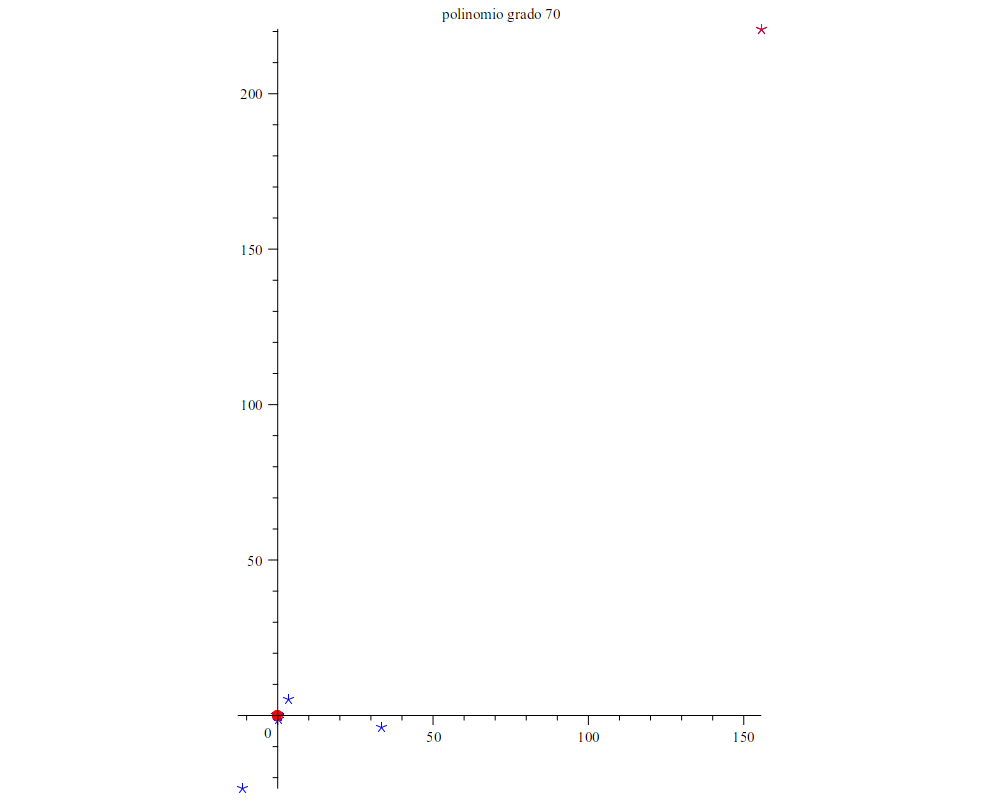
\includegraphics[width=0.9\textwidth]{include/r1_1c1_(-0.5)(-0.5)c2_0_zero.png}

	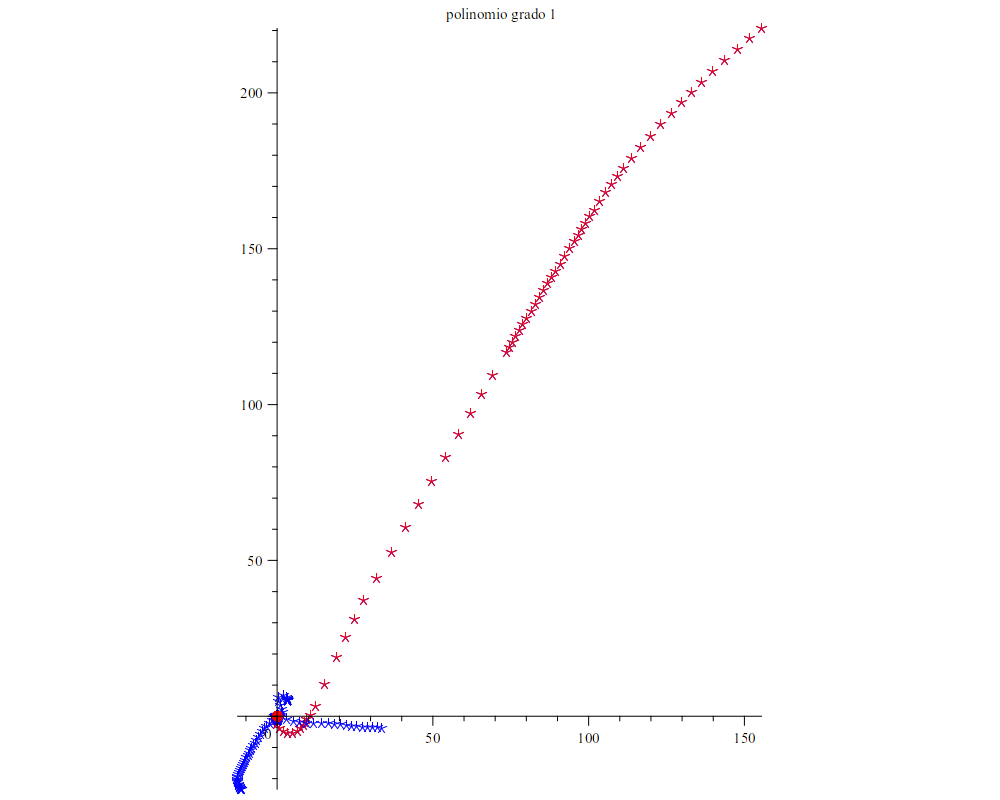
\includegraphics[width=0.9\textwidth]{include/r1_1c1_(-0.5)(-0.5)c2_0_zeros.png}
\end{center}

\begin{enumerate}
	\item $\lim_{n \to 50}\sigma_{1,n}=314.848$
	\item $\lim_{n \to 50} \rho(\mathcal{D}_{n})=270.137$
	\item $\max\{Z_{n}\}_{n=0}^{50}=270.137$
	\item $\lim_{n \to 50}\sigma_{2,n}=54.035$
\end{enumerate}

\textbf{Ejemplo 10.} % Originalmente Ejemplo 7
$\langle p(z),q(z) \rangle=\int_{S_{0}(1)} p(z)\overline{q(z)}\, dm_{0;1} + p'(0.5)\overline{q'(0.5)}$

\begin{center}
	\begin{minipage}{0.48\textwidth}
		\centering
		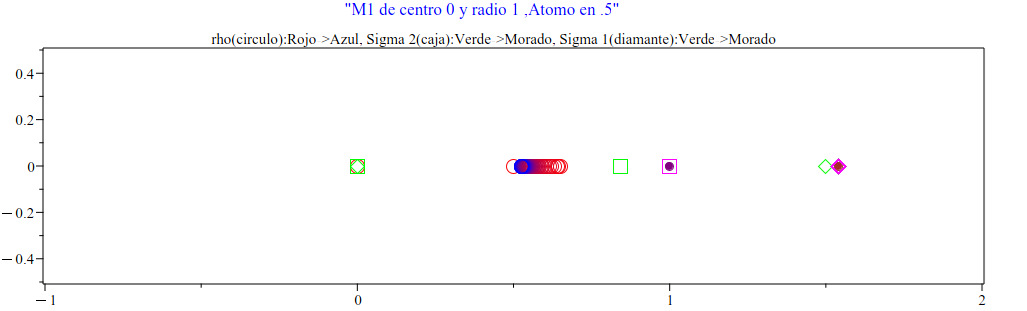
\includegraphics[width=\textwidth]{include/r1_1c1_0c2_0.5.png}
	\end{minipage}%
	\hfill
	\begin{minipage}{0.48\textwidth}
		\centering
		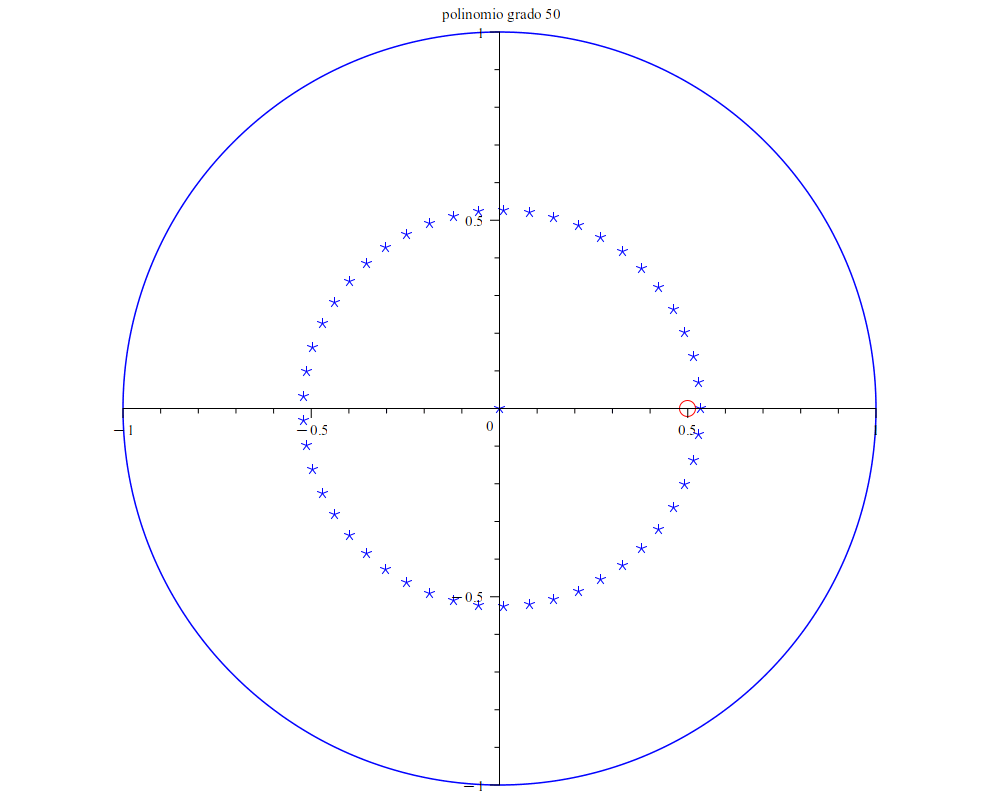
\includegraphics[width=\textwidth]{include/r1_1c1_0c2_0.5_zeros.png}
	\end{minipage}
\end{center}

\begin{enumerate}
	\item $\lim_{n \to 50}\sigma_{1,n}=1.5417$
	\item $\lim_{n \to 50} \rho(\mathcal{D}_{n})=0.5333$
	\item $\max\{Z_{n}\}_{n=0}^{50}=0.6514$
	\item $\lim_{n \to 50}\sigma_{2,n}=1.000$
\end{enumerate}

\textbf{Ejemplo 11.}% Originalmente Ejemplo 7
$\langle p(z),q(z) \rangle=\int_{S_{-0.5}(1)} p(z)\overline{q(z)}\, dm_{-0.5;1} + p'(0)\overline{q'(0)}$

\begin{center}
	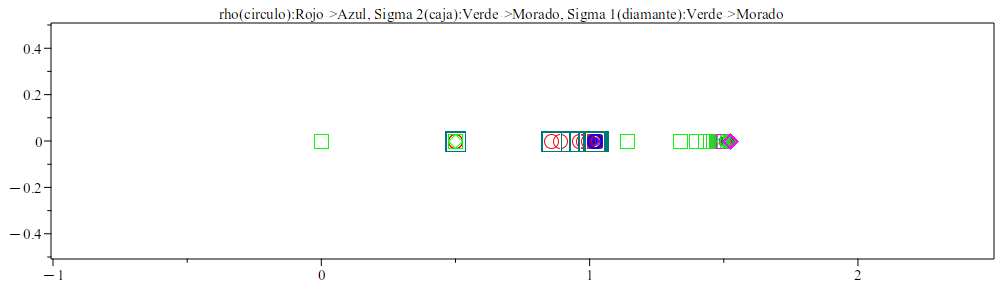
\includegraphics[width=0.9\textwidth]{include/r1_1c1_(-0.5)c2_0.png}

	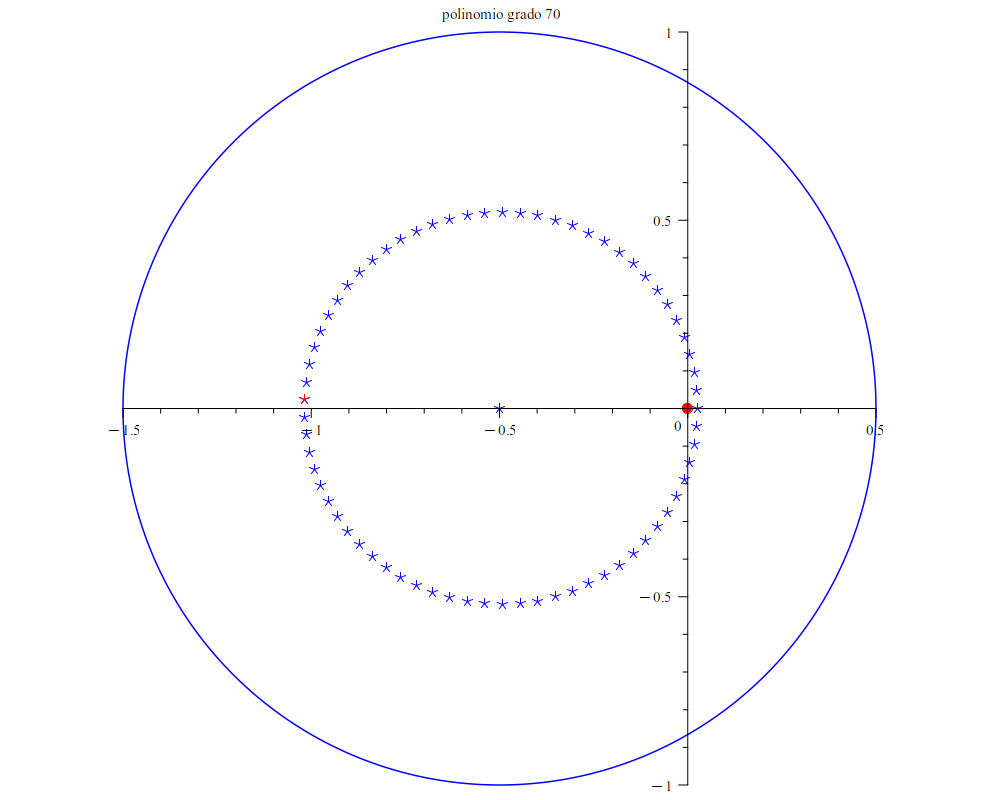
\includegraphics[width=0.9\textwidth]{include/r1_1c1_(-0.5)c2_0_zero.png}

	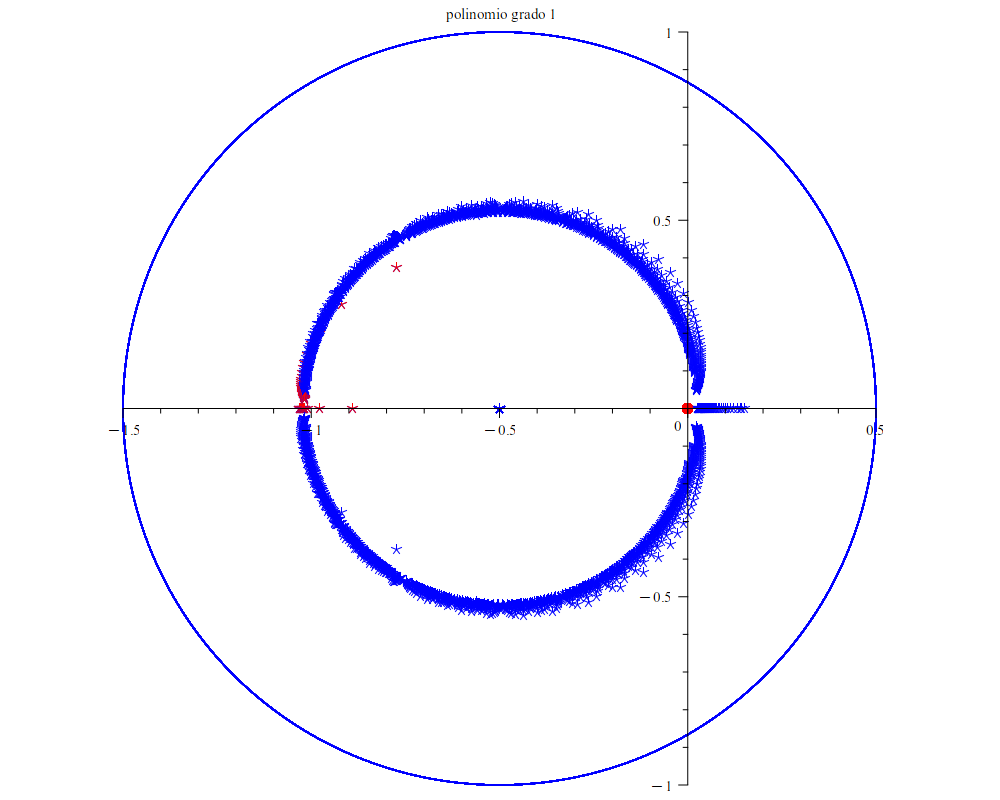
\includegraphics[width=0.9\textwidth]{include/r1_1c1_(-0.5)c2_0_zeros.png}
\end{center}

\begin{enumerate}
	\item $\lim_{n \to 50}\sigma_{1,n}=1.525$
	\item $\lim_{n \to 50} \rho(\mathcal{D}_{n})=1.017$
	\item $\max\{Z_{n}\}_{n=0}^{50}=1.031$
	\item $\lim_{n \to 50}\sigma_{2,n}=1.500$
\end{enumerate}

\textbf{Ejemplo 12.} % Originalmente Ejemplo 8
$\langle p(z),q(z) \rangle=\int_{S_{0}(1)} p(z)\overline{q(z)}\, dm_{0;1} + p'(0)\overline{q'(0)}$

\begin{center}
	\begin{minipage}{0.48\textwidth}
		\centering
		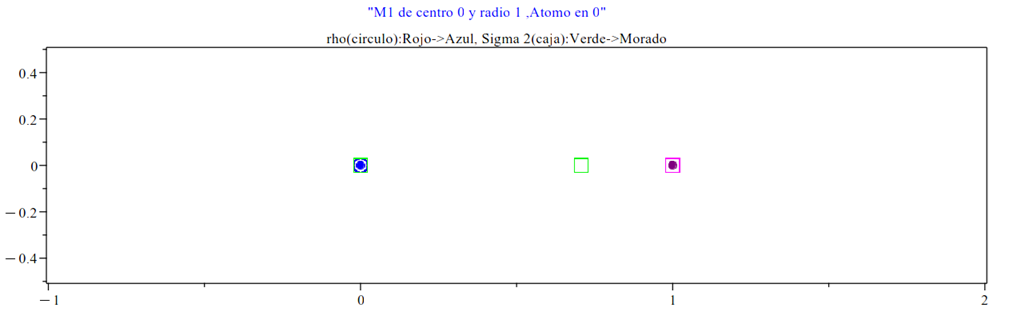
\includegraphics[width=\textwidth]{include/r1_1c1_0c2_0.png}
	\end{minipage}%
	\hfill
	\begin{minipage}{0.48\textwidth}
		\centering
		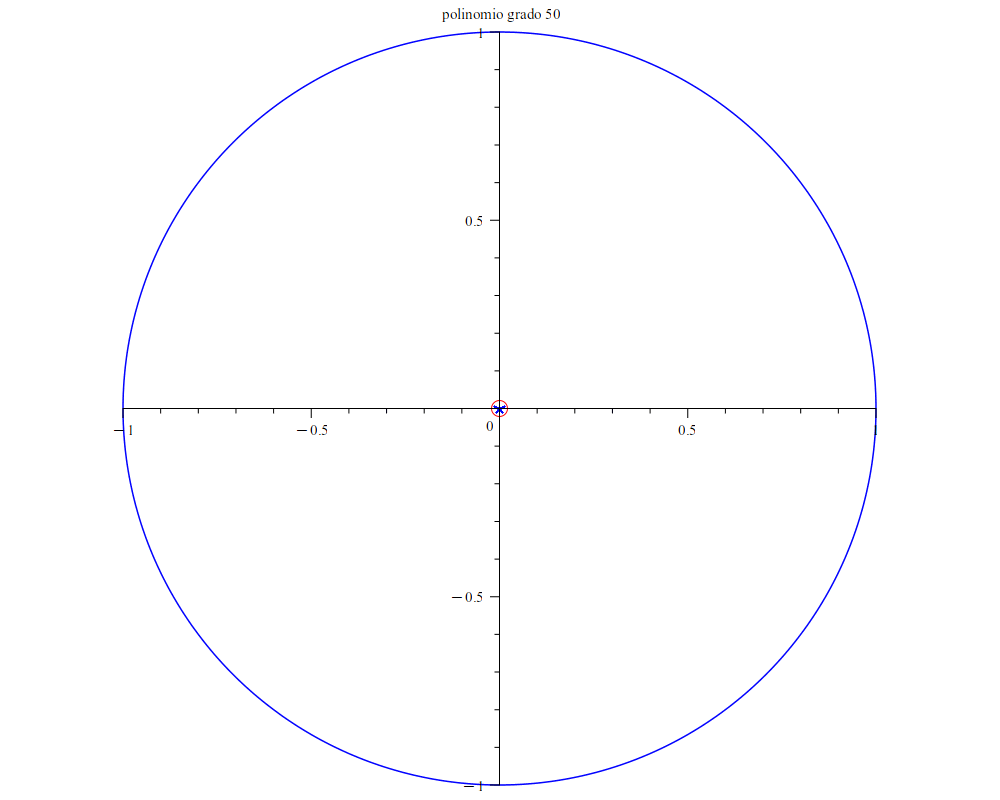
\includegraphics[width=\textwidth]{include/r1_1c1_0c2_0_zeros.png}
	\end{minipage}
\end{center}

\begin{enumerate}
	\item $\lim_{n \to 50}\sigma_{1,n}=1.4142$
	\item $\lim_{n \to 50} \rho(\mathcal{D}_{n})=0.0000$
	\item $\max\{Z_{n}\}_{n=0}^{50}=0.0000$
	\item $\lim_{n \to 50}\sigma_{2,n}=1.000$
\end{enumerate}

\textbf{Ejemplo 13.} % Originalmente Ejemplo 9
$\langle p(z),q(z) \rangle=\int_{S_{0}(1)} p(z)\overline{q(z)}\, dm_{0;1} + p'(0.5i)\overline{q'(0.5i)}$

\begin{center}
	\begin{minipage}{0.48\textwidth}
		\centering
		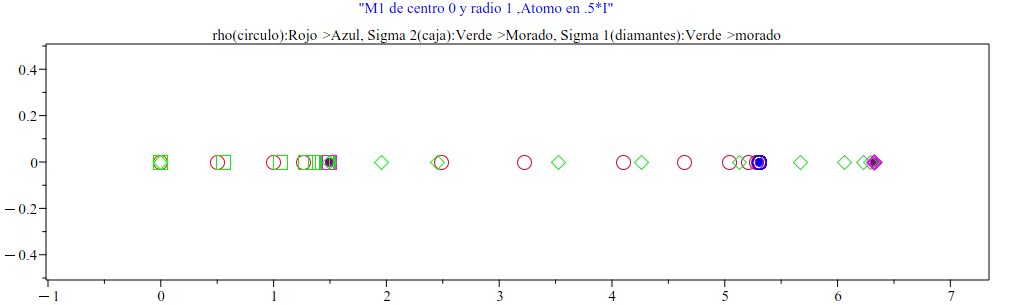
\includegraphics[width=\textwidth]{include/r1_1c1_0c2_(0)(0.5).png}
	\end{minipage}%
	\hfill
	\begin{minipage}{0.48\textwidth}
		\centering
		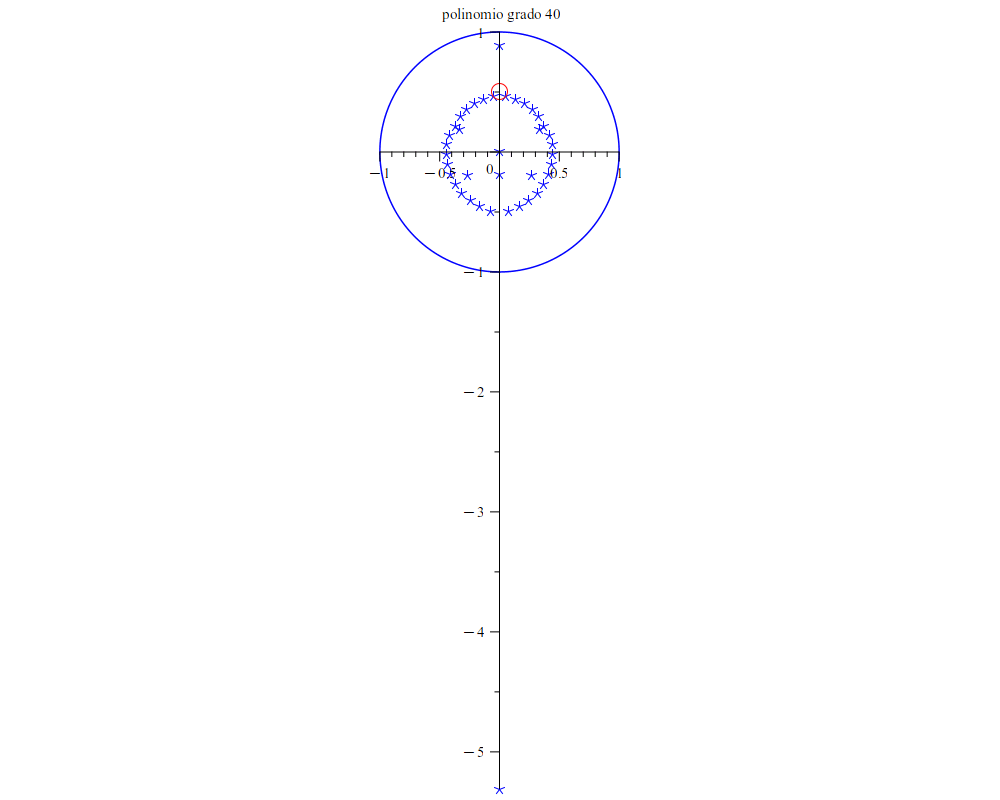
\includegraphics[width=\textwidth]{include/r1_1c1_0c2_(0)(0.5)_zeros.png}
	\end{minipage}
\end{center}

\begin{enumerate}
	\item $\lim_{n \to 50}\sigma_{1,n}=6.3250$
	\item $\lim_{n \to 50} \rho(\mathcal{D}_{n})=5.3106$
	\item $\max\{Z_{n}\}_{n=0}^{50}=5.3106$
	\item $\lim_{n \to 50}\sigma_{2,n}=1.4923$
\end{enumerate}

\textbf{Ejemplo 14.} % Originalmente Ejemplo 9
$\langle p(z),q(z) \rangle=\int_{S_{-0.5i}(1)} p(z)\overline{q(z)}\, dm_{-0.5i;1} + p'(0)\overline{q'(0)}$

\begin{center}
	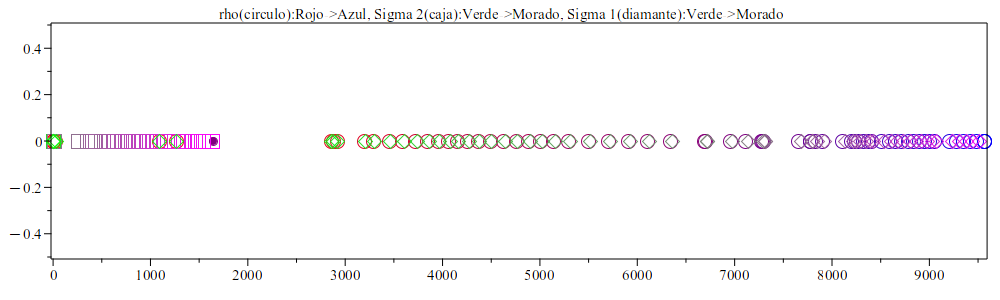
\includegraphics[width=0.9\textwidth]{include/r1_1c1_(-0.5i)c2_0.png}

	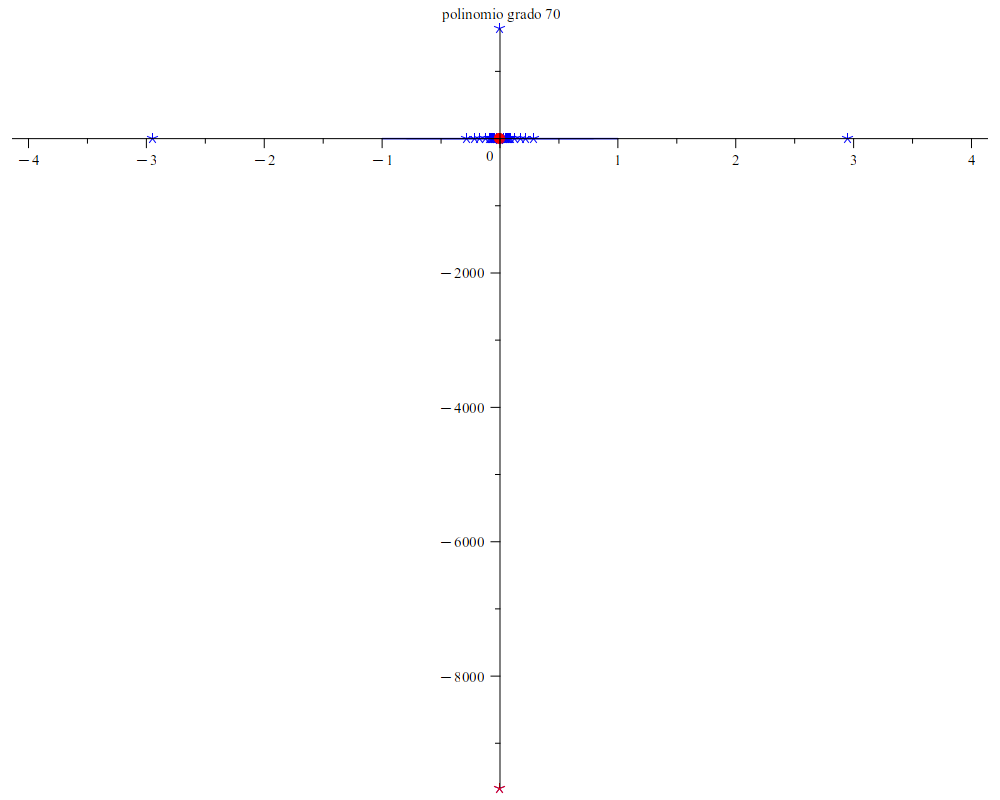
\includegraphics[width=0.9\textwidth]{include/r1_1c1_(-0.5i)c2_0_zero.png}

	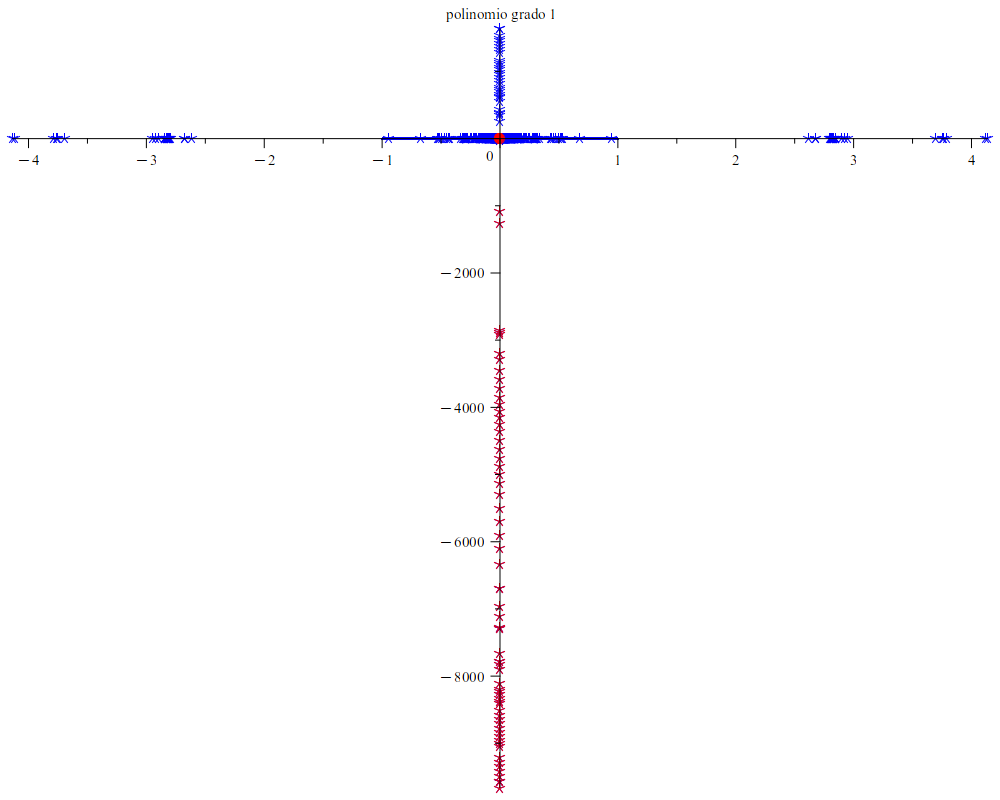
\includegraphics[width=0.9\textwidth]{include/r1_1c1_(-0.5i)c2_0_zeros.png}
\end{center}

\begin{enumerate}
	\item $\lim_{n \to 70}\sigma_{1,n}=9690.60$
	\item $\lim_{n \to 70} \rho(\mathcal{D}_{n})=9665.19$
	\item $\max\{Z_{n}\}_{n=0}^{70}=9665.19$
	\item $\lim_{n \to 70}\sigma_{2,n}=1647.79$
\end{enumerate}

\textbf{Ejemplo 15.} % Originalmente Ejemplo 9
$\langle p(z),q(z) \rangle=\int_{S_{0}(1)} p(z)\overline{q(z)}\, dm_{0;1} + p'(10)\overline{q'(10)}$

\begin{center}
	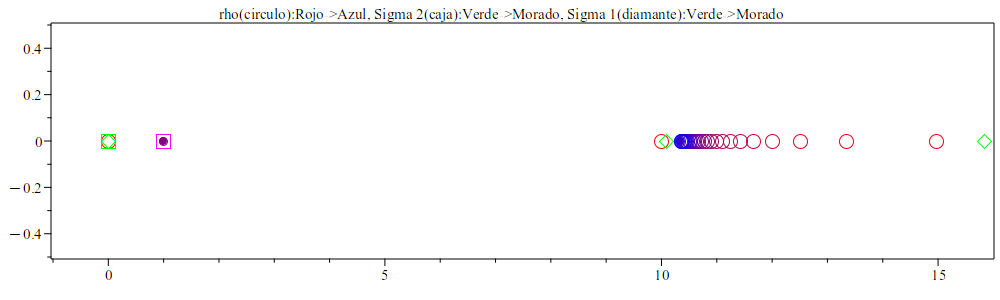
\includegraphics[width=0.9\textwidth]{include/r1_1c1_0c2_10.png}

	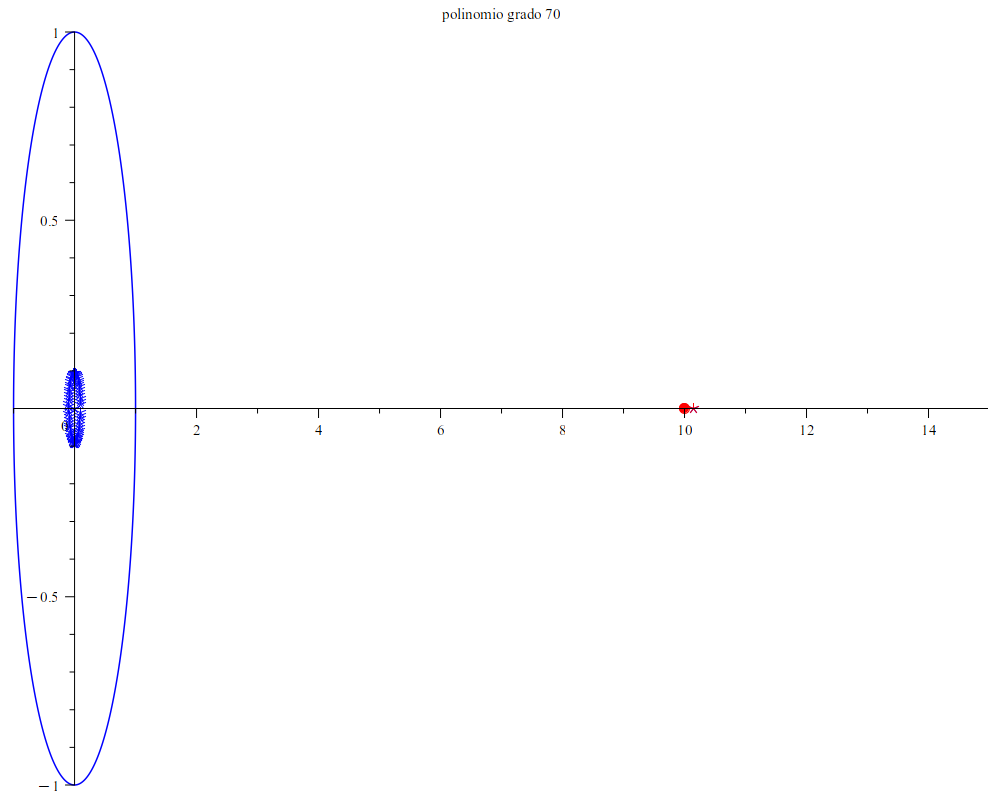
\includegraphics[width=0.9\textwidth]{include/r1_1c1_0c2_10_zero.png}

	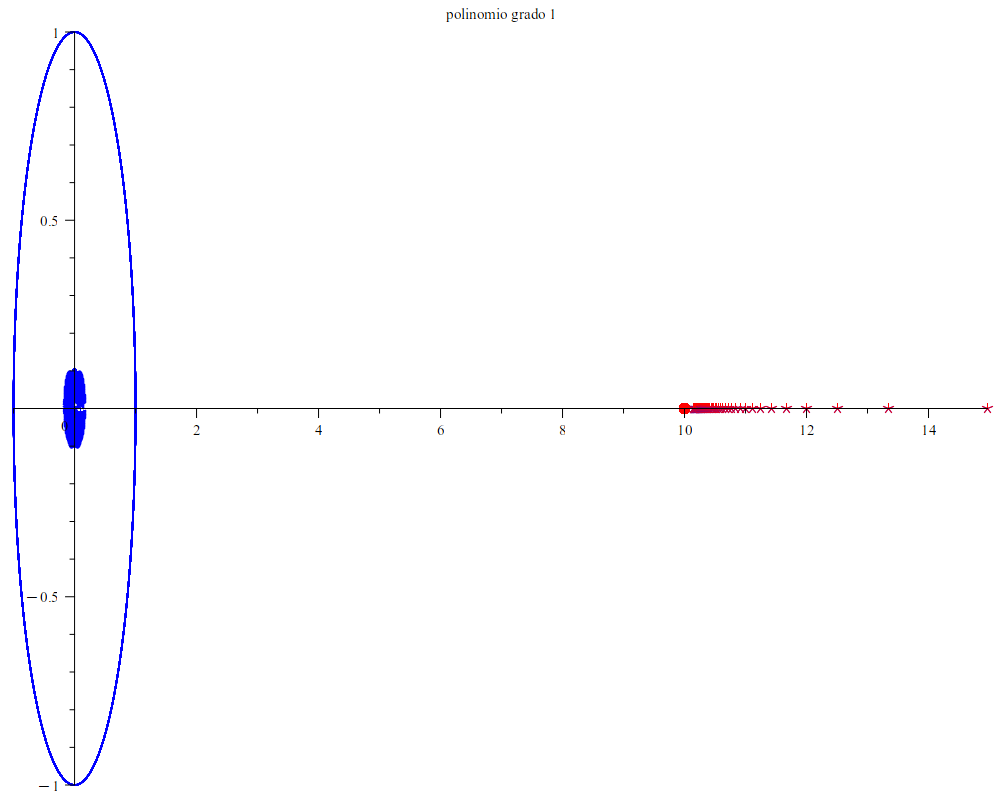
\includegraphics[width=0.9\textwidth]{include/r1_1c1_0c2_10_zeros.png}
\end{center}

\begin{enumerate}
	\item $\lim_{n \to 50}\sigma_{1,n}=3.502\times10^{26}$
	\item $\lim_{n \to 50} \rho(\mathcal{D}_{n})=10.345$
	\item $\max\{Z_{n}\}_{n=0}^{50}=14.975$
	\item $\lim_{n \to 50}\sigma_{2,n}=1.000$
\end{enumerate}

\begin{sidewaystable}
	\centering
	\small
	\caption{Resumen de ejemplos sobre la localización de ceros en el caso de circunferencias.}
	\begin{tabular}{|c|cccc|cccc|cccc|}
		\hline
		\multirow{3}{*}{\textbf{Parámetros}}     & \multicolumn{4}{c|}{\textbf{SECUENCIALMENTE}} & \multicolumn{4}{c|}{\textbf{NO SECUENCIALMENTE}} & \multicolumn{4}{c|}{\textbf{ÁTOMO}}                                                                                                                                                                            \\
		                                         & \multicolumn{4}{c|}{\textbf{DOMINADO}}        & \multicolumn{4}{c|}{\textbf{DOMINADO}}           & \multicolumn{4}{c|}{}                                                                                                                                                                                          \\
		\cline{2-13}
		                                         & $\sigma_{1,n}$                                & $\sigma_{2,n}$                                   & $\rho(\mathcal{D}_{n})$             & $\max Z$ & $\sigma_{1,n}$         & $\sigma_{2,n}$ & $\rho(\mathcal{D}_{n})$ & $\max Z$ & $\sigma_{1,n}$         & $\sigma_{2,n}$ & $\rho(\mathcal{D}_{n})$ & $\max Z$   \\
		\hline
		\textbf{Ej.1}: $S_{0}(1), S_{0.4}(0.4)$  & $1.516$                                       & $1.000$                                          & $0.667$                             & $0.672$  & -                      & -              & -                       & -        & -                      & -              & -                       & -          \\
		\textbf{Ej.2}: $S_{0}(1), S_{0.5}(2)$    & $3.470$                                       & $2.968$                                          & $1.108$                             & $1.112$  & -                      & -              & -                       & -        & -                      & -              & -                       & -          \\
		\textbf{Ej.3}: $S_{0}(1), S_{0.5}(10)$   & $15.248$                                      & $13.972$                                         & $1.068$                             & $1.185$  & -                      & -              & -                       & -        & -                      & -              & -                       & -          \\
		\textbf{Ej.4}: $S_{0}(1), S_{1}(1)$      & -                                             & -                                                & -                                   & -        & $2.672$                & $2.672$        & $1.933$                 & $1.963$  & -                      & -              & -                       & -          \\
		\textbf{Ej.5}: $S_{0}(1), S_{-10}(1)$    & -                                             & -                                                & -                                   & -        & $4.963 \times 10^{14}$ & $11.211$       & $12.424$                & $15.074$ & -                      & -              & -                       & -          \\
		\textbf{Ej.6}: $S_{-10}(0.25), S_{0}(1)$ & -                                             & -                                                & -                                   & -        & $9.660 \times 10^{22}$ & $10.249$       & $10.035$                & $10.035$ & -                      & -              & -                       & -          \\
		\textbf{Ej.7}: $S_{0}(1), S_{-10}(0.25)$ & -                                             & -                                                & -                                   & -        & $1.409 \times 10^{23}$ & $10.298$       & $11.641$                & $14.981$ & -                      & -              & -                       & -          \\
		\textbf{Ej.8}: $S_{0}(1), c=0.5+0.5i$    & -                                             & -                                                & -                                   & -        & -                      & -              & -                       & -        & $33.560$               & $1.457$        & $31.489$                & $31.489$   \\
		\textbf{Ej.9}: $S_{-0.5-0.5i}(1), c=0$   & -                                             & -                                                & -                                   & -        & -                      & -              & -                       & -        & $314.848$              & $54.035$       & $270.137$               & $270.137$  \\
		\textbf{Ej.10}: $S_{0}(1), c=0.5$        & -                                             & -                                                & -                                   & -        & -                      & -              & -                       & -        & $1.542$                & $1.000$        & $0.533$                 & $0.651$    \\
		\textbf{Ej.11}: $S_{-0.5}(1), c=0$       & -                                             & -                                                & -                                   & -        & -                      & -              & -                       & -        & $1.525$                & $1.500$        & $1.017$                 & $1.031$    \\
		\textbf{Ej.12}: $S_{0}(1), c=0$          & -                                             & -                                                & -                                   & -        & -                      & -              & -                       & -        & $1.414$                & $1.000$        & $0.000$                 & $0.000$    \\
		\textbf{Ej.13}: $S_{0}(1), c=0.5i$       & -                                             & -                                                & -                                   & -        & -                      & -              & -                       & -        & $6.325$                & $1.492$        & $5.311$                 & $5.311$    \\
		\textbf{Ej.14}: $S_{-0.5i}(1), c=0$      & -                                             & -                                                & -                                   & -        & -                      & -              & -                       & -        & $9690.600$             & $1647.790$     & $9665.190$              & $9665.190$ \\
		\textbf{Ej.15}: $S_{0}(1), c=10$         & -                                             & -                                                & -                                   & -        & -                      & -              & -                       & -        & $3.502 \times 10^{26}$ & $1.000$        & $10.345$                & $14.975$   \\
		\hline
	\end{tabular}
\end{sidewaystable}

\newpage

\section{Análisis y Conjeturas}

El Cuadro 2.1, que resume los experimentos numéricos para el caso real, revela una variedad de comportamientos. Notablemente, en ejemplos como el primero, donde el producto de Sobolev puede considerarse secuencialmente dominado (es decir, el soporte de la integral que involucra las derivadas, $I_2=[c,d]$, está contenido en el soporte de la integral del término sin derivadas, $I_1=[a,b]$, y el cociente de los pesos $w_1(t)/w_0(t)$ está acotado en $I_1$), los valores singulares del operador de multiplicación truncado $\mathbf{D}_n$ y su radio espectral sugieren la acotación del operador $\mathcal{D}$. La Proposición \ref{prop:bounded_operator_continuous} aborda formalmente esta situación, estableciendo una cota para la norma de $\mathcal{D}$ bajo dichas condiciones de dominación secuencial en el caso real continuo.

\begin{proposition}\label{prop:bounded_operator_continuous}
	Para el caso continuo real secuencialmente dominado con soportes $I_1=[a,b]$ y $I_2=[c,d]$ con $[c,d] \subset [a,b]$, definamos
	\(
	R = \max\{|a|,|b|,|c|,|d|\},
	\qquad
	\alpha = \max_{t\in[a,b]}\frac{w_1(t)}{w_0(t)}.
	\)
	Entonces el operador multiplicación $\mathcal{D}$
	es acotado en el producto Sobolev y satisface
	\(
	\|\mathcal{D}\|\;\le\;\sqrt{2(R^{2}+\alpha)}\,.
	\)
\end{proposition}

\begin{proof}
	Sea $p(t)\in\mathbb{P}[t]$.
	\noindent Utilizando que $(a+b)^2\leq 2(a^2+b^2)$ para $a,b\ge0$, se obtiene:
	$$
		\Vert \mathcal{D}(p(t))\Vert^{2}
		= \int_{a}^{b} t^2 p^2(t) w_0(t)\,dt
		\;+\;\int_{c}^{d} \Bigl[(tp(t))'\Bigr]^2 w_1(t)\,dt
	$$
	$$
		= \int_{a}^{b} t^2 p^2(t) w_0(t)\,dt
		+ \int_{c}^{d} \Bigl(p(t)+tp'(t)\Bigr)^2 w_1(t)\,dt
		\;\le\;
	$$
	$$
		\int_{a}^{b} t^2p^2(t)w_0(t)\; dt+2\Bigl(\int_{c}^{d} p(t)^2w_1(t)\; dt +\int_{c}^{d} t^2p'(t)^2w_1(t)\; dt\Bigr) \leq
	$$
	$$
		R^{2} \Bigl(\int_{a}^{b} p^2(t)w_0(t)\; dt +  2\int_{c}^{d} p'(t)^2w_1(t)\; dt\Bigr)+ 2\int_{c}^{d} p(t)^2w_1(t)\; dt \leq
	$$
	$$
		2R^{2} \Vert p(t)\Vert^{2} + 2\alpha \int_{c}^{d} p(t)^2w_0(t)\; dt \leq 2R^{2} \Vert p(t)\Vert^{2} + 2\alpha \int_{a}^{b} p(t)^2w_0(t)\; dt
	$$
	$$
		2(R^{2}+\alpha)\Vert p(t) \Vert^{2}
	$$

\end{proof}

\noindent Por ejemplo, si $[a,b]=[c,d]=[-1,1]$ y $\alpha=1$, entonces
$\|\mathcal{D}\|\le\sqrt{2+2}=\sqrt{4}=2$.

\todo{reordenar analisis}
\begin{itemize}
	\item El segundo mayor valor singular de $\mathcal{D}_{n}$ converge al extremo con mayor módulo de los soportes. Se puede encontrar una constante de proporción o de desviacion $K$ que depende de los soportes (extremos,intersección, tamaño) para poder acotar los ceros.
	\item $\lim_{n \to \infty} \max{Z_n}=\max\{|a|,|b|,|c|,|d|\} + k = \max\{|a|,|b|,|c|,|d|\} \cdot k'$
	\item El $k$ cuando $\max\{|a|,|b|\} < \max\{|c|,|d|\}$ es notablemente mayor que el $k$ cuando ocurre lo contrario.
	\item $k$ o $k'$ depende de la posición relativa entre los soportes.
	      \begin{itemize}
		      \item Si $[a,b] \cap [c,d] = \emptyset$ y $dist(b,c) < dist(a,b) + dist(c,d)$ entonces $k$ o $k'$ no crece mucho.
		      \item Si $[a,b] \cap [c,d] = \emptyset$ y $dist(b,c) > dist(a,b) + dist(c,d)$ entonces $k$ o $k'$ crece mucho.
		      \item Si $[a,b] \cap [c,d] \neq \emptyset$ entonces $k$ o $k'$ crece muy poco. Mientras mayor sea $dist(b,c)$ menos crece $k$ o $k'$.
	      \end{itemize}
\end{itemize}

Dejando de lado los productos de Sobolev, consideremos el producto interno de la forma:
$$\langle p(t),q(t) \rangle = \int_{a}^{b} p(t) q(t) \, dt + |p'(c)||q'(c)|.$$
Este producto interno es muy interesante ya que solo introduce un átomo al producto interno usual, y sin embargo el operador multiplicación no es acotado. En los siguientes ejemplos se mostrará que los ceros de los polinomios ortogonales asociados a este producto interno están acotados, y que podemos encontrar una cota.

A raíz de estos ejemplos podemos conjeturar lo siguiente:

\begin{itemize}
	\item Si $c \in [a,b]$ entonces los ceros convergen al límite del soporte, y podemos usar el segundo mayor valor singular como cota.
	\item Si $c \notin [a,b]$ entonces los ceros convergen al átomo, y podemos usar el átomo como cota. Pero necesitamos determinar el coeficiente $k$ para poder abarcar todos los ceros.
\end{itemize}

\begin{proposition}
	\todo{Poner el resultado de traslacion de los ceros, por lo que se trasladara atomo al 0}
\end{proposition}

\begin{conjetura}
	Para los 4 casos (1.3)-(1.6) se tiene que
	$$
		\lim_{n \to \infty} \rho(\mathbf{D}_n) < \infty
	$$
\end{conjetura}

\paragraph{Resultado}
En todos los ejemplo se tiene que $\lim_{n \to \infty} \sigma_{2,n} < \infty$.

\begin{conjetura}
	Para los 4 casos (1.3)-(1.6) se tiene que si $\lim_{n \to \infty} \sigma_{1,n} < \infty$ entonces
	$$
		\lim_{n \to \infty} \sigma_{2,n} < \infty
	$$
\end{conjetura}

\noindent Veamos un resultado que apoya a la conjetura.

\noindent {\bf Teorema de entrelazamiento de Cauchy} Sea  $A$ una matriz de orden  $n$ y sea  $B$ una submatriz principal de  $A$ de  orden  $n-1$. Si $\lambda_n\leq \dots \leq \lambda_2\leq \lambda_1$ son los autovalores de $A$ y  $\mu_{n-1}\leq \dots \leq \mu_2\leq \mu_1$ son los autovalores de  $B$ entonces
$$
	\lambda_n \leq \mu_{n-1} \leq \dots \leq \mu_2 \leq \lambda_1.
$$


\begin{proposition} Sea $\mathbf{M}$ HPSD. Sean

	$$
		0 \leq \lambda_{n,n}\leq \dots \lambda_{2,n} \leq \lambda_{1,n}.
	$$
	\noindent los autovalores de la matriz $\mathbf{M}_n$. Entonces La sucesión $\{ \lambda_{2,n}\}_{n=1}^{\infty}$ es una sucesión creciente, es decir,
	$$
		\lambda_{2,n+1} \leq \lambda_{2,n} \qquad \forall n\in \mathbb{N}.
	$$
	\noindent por lo que existe $\displaystyle{\lim_{n\to \infty} \lambda_{2,n}}$ pudiendo ser finito o infinito.
\end{proposition}


\begin{proof} Utilizando el teorema de entrelazamiento se tiene que:

	$$
		0 \leq \lambda_{n+1,n+1} \leq \lambda_{n,n} \lambda_{n,n+1} \leq \dots \lambda_{2,n}  \leq \lambda_{2,n+1} \leq \lambda_{1,n} \leq \lambda_{1,n+1}
	$$

	\noindent En particular,
	$$
		\lambda_{2,n+1} \leq \lambda_{2,n} \qquad \forall n\in \mathbb{N}.
	$$
\end{proof}

\noindent

\begin{lemma} Sea $\mathbf{D}$ una matriz infinita de Hessemberg superior y $\mathbf{D}_n$ las secciones de orden $n+1$. Entonces se tiene que
	\begin{enumerate}

		\item $$
			      (\mathbf{D}_{n+1}^{*}\mathbf{D}_{n+1})_{n} = \mathbf{D}_n^{*}\mathbf{D}_n
		      $$
		\item
		      $$(\mathbf{D}^{*}\mathbf{D})_{n}= \mathbf{D}_n^{*}\mathbf{D}_n
		      $$

	\end{enumerate}
\end{lemma}

\noindent ES POSIBLE ENCONTRAR UNA REFERENCIA DE ESTE RESULTADO EN LOS TRABAJOS DE EMILIO.

\begin{proposition}
	Sea $\mathbf{D}$ una matriz infinita de Hessemberg, y $\mathbf{D}_n$ las secciones de orden $n$ entonces si $$
		0 \leq \sigma_{n,n}\leq \dots \sigma_{2,n} \leq \sigma_{1,n}.
	$$

	\noindent los valores singulares de la matriz $\mathbf{D}_n$ se tiene que
	la sucesión $\{\sigma_{2,n}\}_{n=1}^{\infty}$ es creciente y existe
	$$
		\lim_{n\to \infty} \sigma_{2,n} \leq \infty
	$$


\end{proposition}

\todo{poner resultado entrelazamiento y terminar de formalizar conjeturas}

\todo{cuando el centro de la segunda circunferencia está dentro del disco abierto de la primera, la D esta acotada, y cuando esta fuera no se sabe que pasa.}